\documentclass[default,iicol]{sn-jnl}

\usepackage{amsmath}
\usepackage{array}
\usepackage[acronym]{glossaries}
\usepackage{epsfig} %% for loading postscript figures
\usepackage{float}
\usepackage[utf8]{inputenc}
\usepackage{siunitx}
\usepackage{stfloats}
\usepackage{subfig}
\usepackage{titlesec}
\usepackage{url}
\usepackage{xcolor}

\setcounter{secnumdepth}{4}

\titleformat{\paragraph}
{\normalfont\normalsize\bfseries}{\theparagraph}{1em}{}
\titlespacing*{\paragraph}
{0pt}{3.25ex plus 1ex minus .2ex}{1.5ex plus .2ex}

%\def\url#1{\expandafter\string\csname #1\endcsname}
\newcounter{exno}
\newenvironment{examples}
{
\begin{flushleft}
\begin{tabular}{>{(\refstepcounter{exno}\theexno\label{row:\theexno}) }rl}
}
{
\end{tabular}
\end{flushleft}
}
%\newcommand*{\@rowstyle}{}
\newcommand*{\rowstyle}[1]{% sets the style of the next row
  \gdef\@rowstyle{#1}%
  \@rowstyle\ignorespaces%
}
\newcolumntype{=}{% resets the row style
  >{\gdef\@rowstyle{}}%
}
\newcolumntype{+}{% adds the current row style to the next column
  >{\@rowstyle}%
}
\definecolor{ao}{rgb}{0.0, 0.5, 0.0}
\definecolor{coolblack}{rgb}{0.0, 0.18, 0.39}

\glsdisablehyper
\newacronym[longplural={centers of mass}]{com}{CoM}{center of mass}
\newacronym[longplural={equations of motion}]{eom}{EoM}{equation of motion}
\newacronym{ocp}{OCP}{optimal control problem}
\newacronym{grf}{GRF}{ground reaction force}
\newacronym{vgrf}{VGRF}{vertical ground reaction force}
\newacronym{nlp}{NLP}{non-linear programming problem}
\newacronym[longplural={degrees of freedom}]{dof}{DoF}{degree of freedom}
\newacronym{rfd}{RFD}{rate of force development}
\newacronym{cmj}{CMJ}{countermovement jump}

% \usepackage{fancyhdr}% http://ctan.org/pkg/fancyhdr

% % \fancyhf{}% Clear header/footer
% % \fancyhead[R]{\sectionmark}
% % \fancyfoot[C]{\thepage}% \fancyfoot[R]{\thepage}
% % \renewcommand{\headrulewidth}{0.4pt}% Default \headrulewidth is 0.4pt

% % \renewcommand{\sectionmark}[1]{\markright{\thesection~- ~#1}}
% % \renewcommand{\chaptermark}[1]{\markboth{\chaptername~\thechapter~-~ #1}{}}
% \renewcommand{\subsectionmark}[1]{\markright{#1}}

% %\usepackage[T1]{fontenc}
% \usepackage{bold-extra}


% % % Fancyhdr setup
% % \pagestyle{fancy}% Change page style to fancy
% % \fancyhf{} % clear all header fields
% % \fancyhead[L]{\footnotesize\scshape\leftmark}
% % \fancyhead[R]{\footnotesize\scshape\rightmark}
% % \fancyfoot[C]{\thepage}
% % \renewcommand{\headrulewidth}{0.4 pt}
% % \renewcommand{\footrulewidth}{0 pt}

\newcounter{magicrownumbers}
\newcommand\rownumber{\stepcounter{magicrownumbers}\arabic{magicrownumbers}}

\jyear{2021}%

\raggedbottom
%%\unnumbered% uncomment this for unnumbered level heads

\begin{document}

\title[Optimal Skateboard Geometry for Maximizing Ollie Height]{
  Optimal Skateboard Geometry for Maximizing Ollie Height}

%%=============================================================%%
%% Prefix	-> \pfx{Dr}
%% GivenName	-> \fnm{Joergen W.}
%% Particle	-> \spfx{van der} -> surname prefix
%% FamilyName	-> \sur{Ploeg}
%% Suffix	-> \sfx{IV}
%% NatureName	-> \tanm{Poet Laureate} -> Title after name
%% Degrees	-> \dgr{MSc, PhD}
%% \author*[1,2]{\pfx{Dr} \fnm{Joergen W.} \spfx{van der} \sur{Ploeg} \sfx{IV} \tanm{Poet Laureate} 
%%                 \dgr{MSc, PhD}}\email{iauthor@gmail.com}
%%=============================================================%%

\author*[1]{\fnm{Jan T.} \sur{Heinen}}\email{janheinen97@gmail.com}
\equalcont{These authors contributed equally to this work.}

\author[1]{\fnm{Samuel G.} \sur{Brockie}}\email{s.g.brockie@tudelft.nl}
\equalcont{These authors contributed equally to this work.}

\author[1]{\fnm{Raymund} \sur{ten Broek}}\email{raymund@uspc.nl}
\equalcont{These authors contributed equally to this work.}

\author[1]{\fnm{Eline} \sur{van der Kruk}}\email{e.vanderkruk@tudelft.nl}
\equalcont{These authors contributed equally to this work.}

\author[1]{\fnm{Jason K.} \sur{Moore}}\email{j.k.moore@tudelft.nl}
\equalcont{These authors contributed equally to this work.}

\affil*[1]{\orgdiv{Department of Biomechanical Engineering}, \orgname{TU Delft}, \orgaddress{\street{Leeghwaterstraat}, \postcode{2628 CN}, \city{Delft}, \country{Netherlands}}}

%\abstract{
%  Skateboarding involves a human controlling a four wheeled vehicle that is
%  steered by tilting the standing surface. The riding mechanics of
%  skateboarding have been well reported
%  \cite{varszegi_stabilizing_2016}. The sport also
%  includes aerial maneuvers such as jumping of stairs, flying off ramps and
%  flipping and rotating the skateboard. The most basic aerial trick is called
%  the ollie. The athlete jumps up while pushing down on the back end of the
%  skateboard’s tail, causing a rotation about the back axle. The upward
%  acceleration due to the rotation together with the tail-ground impact cause
%  the skateboard to go airborne. Midair the athlete drags the skateboard up
%  through frictional contact and levels it out to land the trick. The most
%  concrete performance measure of the ollie is height according to the Olympic
%  judging criteria\cite{world_skate_skateboarding_2021}. To reach maximum
%  height the dynamics such as impact, dynamic response, and torque production
%  are dependent on shape, inertia and mass, which gives reason to assume an
%  optimal shape exists. This leads to the research question: What are the
%  optimal geometric and inertial parameters of a skateboard for an Olympic
%  athlete to reach maximal ollie height. The skateboard geometry is optimized
%  through multiphase direct collocation with the objective of maximal ollie
%  height. A parameterized model is created with scaling mass and inertia
%  properties such that the geometry of the skateboard. Modelling the dynamics
%  of the ollie including impact and friction are done with a point mass human
%  controller that is kineticly and kinematicly mapped to a counter movement
%  jump. A simplistic contact implicit impact scheme is made for a higher order
%  optimization. The ollie height is improved by changing the mass and inertia
%  properties of the skateboard.  Multiple optimal board shapes are generated
%  for example a skateboard with a smaller wheelbase can reach higher ollie
%  height compared to an industry standard skateboard.
%}

\keywords{Skateboarding, Optimal Control, Parameter Optimization, Direct Collocation}
\maketitle

\section{Introduction}\label{s_intro}

In 1978 Alan `Ollie' Gelfand invented the `no-hand aerial', by riding off an inclined surface and jumping in the air with a skateboard.
Four years later, Rodney Mullen debuted the first ollie from flat ground.
Because the skateboard is not tethered to the skater, an ollie requires a precise sequence of movements to keep the two together~\cite{frederick_biomechanics_2006}.
The maneuver can be deconstructed into the six
distinct phases shown in figure~\ref{fig:ollie steps}.

\begin{figure*}[!t]
\captionsetup[subfigure]{labelformat=empty}
  \subfloat[$t_1$=0.013]{{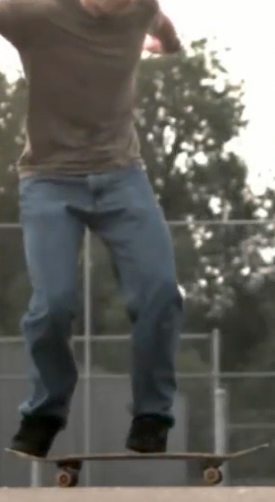
\includegraphics[width=0.13\textwidth]{figure/1.png} }}%
  \subfloat[$t_2$=0.129]{{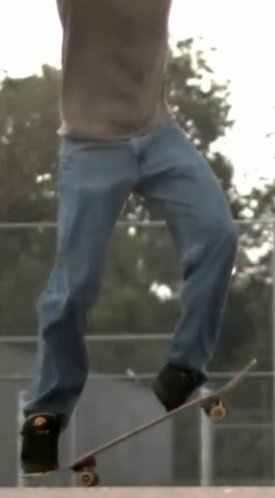
\includegraphics[width=0.13\textwidth]{figure/2.png} }}%
  \subfloat[$t_3$=0.181]{{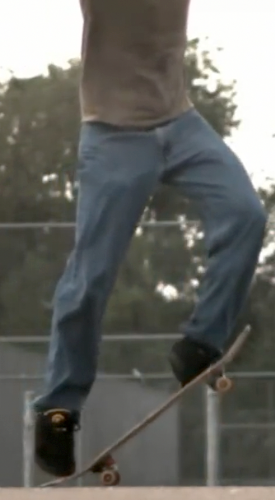
\includegraphics[width=0.13\textwidth]{figure/3.png} }}%
  \subfloat[$t_4$=0.187]{{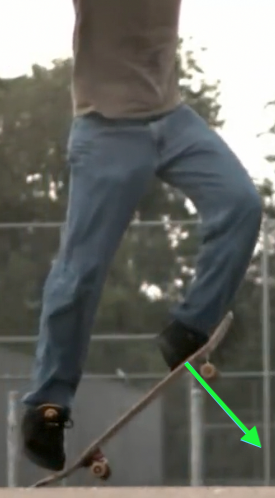
\includegraphics[width=0.13\textwidth]{figure/4.png} }}%
  \subfloat[$t_5$=0.303]{{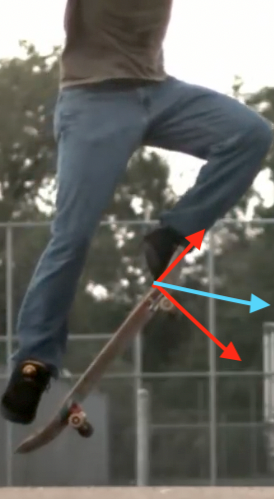
\includegraphics[width=0.13\textwidth]{figure/5.png} }}%
  \subfloat[$t_6$=0.431]{{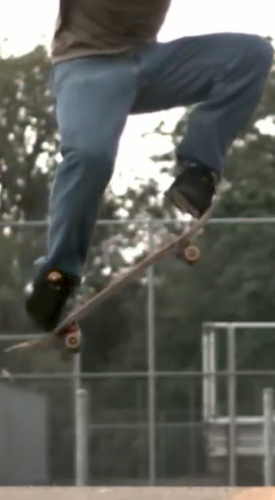
\includegraphics[width=0.13\textwidth]{figure/6.png} }}%
  \subfloat[$t_7$=0.543]{{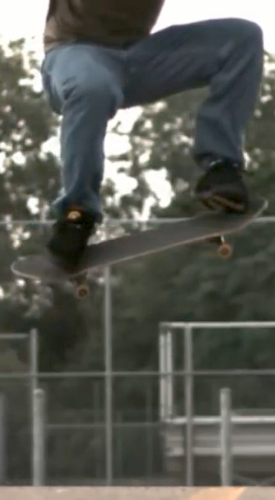
\includegraphics[width=0.13\textwidth]{figure/7.png} }}%
  \protect\newline
  \centering
  \subfloat[$t_8$=0.676$^1$]{{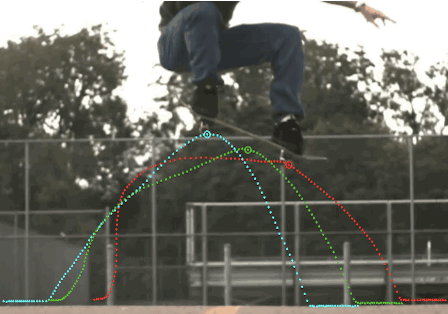
\includegraphics[width=0.336\textwidth]{figure/ollie_tracking_mid.png} }}
  \subfloat[$t_9$=0.722]{{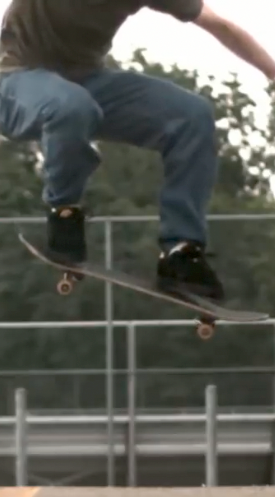
\includegraphics[width=0.13\textwidth]{figure/9.png} }}%
  \subfloat[$t_{10}$=0.904]{{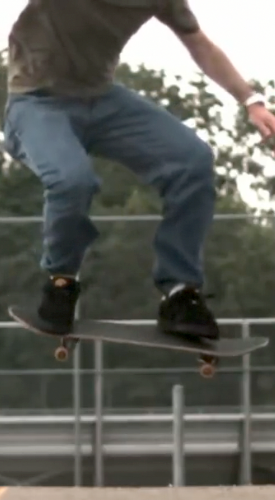
\includegraphics[width=0.13\textwidth]{figure/10.png} }}%
  \subfloat[$t_{11}$=1.097]{{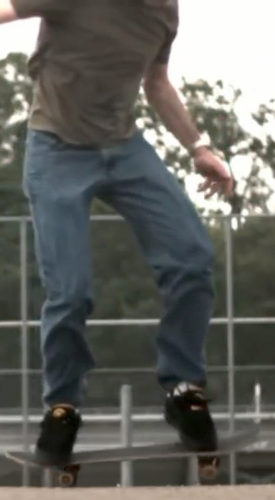
\includegraphics[width=0.13\textwidth]{figure/11.png} }}%
  \captionsetup{singlelinecheck=off}
\footnotesize
    \begin{center}
    \begin{tabular}{p{1.4cm} p{0.75cm} p{12.5cm}}
        \toprule
        Phase & Motion Cue & Description \\
        \midrule
        Preparation     & $t_1$ & The skater lowers their \gls{com} preparing to jump. \\
        Pre-pop         & $t_2$ & The skater pushes firmly from their back leg and is decreasing downward force on the front foot, which results in the front wheels leaving the ground, simultaneously sliding the front foot forward. \\
        Pop             & $t_3$ & Tail collides with the ground, the front foot is still sliding and the back foot is barely in contact with the skateboard~\cite{determan_kinetics_2006,nakashima_simulation_2021}. \\
        Upward motion   & $t_4$ & Back foot is no longer in contact with the skateboard, the back wheels are not in contact with the ground anymore~\cite{determan_kinetics_2006,nakashima_simulation_2021}. \\
                        & $t_5$ & The front foot reached the nose of the skateboard. \\
                        & $t_6$ & Back foot contacts the board again. \\
                        & $t_7$ & Board is leveled out by the front foot. \\
                        & $t_8$ & Highest point is reached. Knees are fully tucked in, the biomechanical obstruction restricts the board from gaining height. Feet are firmly placed on the deck. \\
        Downward motion & $t_9$ & Front foot loses contact. \\
                        & $t_{10}$& Board is horizontal, both feet are in contact. \\
        Landing         & $t_{11}$& The back wheels touch the ground and legs are almost fully stretched out. \\
        \bottomrule
    \end{tabular}
    \end{center}
 \caption[Ollie motion cues]{
    Green arrow: resultant force without friction, red arrows: force components
    with friction, blue arrow: resultant force with friction. Blue-, green- and
    red line are trajectory of back wheel, middle and front wheel respectively. Images are retrieved from \url{youtu.be/339k4XEvbxY} with consent.
  }
  \label{fig:ollie steps}
\end{figure*}

From the early 1960s, new skateboarding pursuits and their differing performance requirements evolved a variety of skateboard shapes.
For example, slalom demanded short boards for quick turns, downhill preferred longboards for stability, and pool skating resulted in wide, concave boards for maximum foothold. 
Artistic motives shaped impractical coffin- and
fish-like boards~\cite{prentiss_get_2011}.
The prevailing modern board shape, used by all Olympic athletes, is the popsicle stick.
The shape supports freestyling, where the ollie is a foundational trick.

There is no standardization of boards in the skateboard industry.
Boards are measured differently by each brand~\cite{johnny_skateboarding_2013} and non-specific descriptions such as mellow, steep, and wide are usually used to communicate deck dimensions to customers~\cite{berger_handmade_2021}.
This makes it difficult for skaters to find their optimal board shape.

Skaters know and feel when a specific skateboard performs to their liking.
However, they do not know how this translates to quantifiable dimensions.
Skateboards might have evolved to optimum geometries over the years, but from an academic and mechanical point of view, skateboard designs have not been shown to be optimal for specific tricks.

Researchers analyze the skateboard in planar riding models~\cite{hubbard_lateral_1979,hubbard_human_1980,kremnev_nonlinear_2010,ispolov_skateboard_1996,rosatello_skateboard_2015,varszegi_stability_2017,varszegi_stabilizing_2016,varszegi_downhill_2016,varszegi_balancing_2014,kuleshov_mathematical_2007,kuleshov_various_2010}, which show the relationship between the dimensions and the stability while rolling and turning. 
However, these dimensional analyses do not apply to aerial movements like the ollie.
Others research the ollie by investigating the contact forces~\cite{anderson_ollie_2020,shield_contact-implicit_2022} and biomechanics~\cite{frederick_biomechanics_2006,vorlicek_analysis_2015,wood_3d_2020,nakashima_simulation_2021,nevitt_ground_2006,candotti_lower_2012,dias_using_2016,anderson_ollie_2020,bridgman_human_1992,ou_postural_2021}.
Two papers have optimized the ollie without changing the geometry~\cite{anderson_ollie_2020,shield_contact-implicit_2022}, but no research has yet shown how the skateboards' dimensions influence the ollie.
Such research would benefit the skateboarding community.

Now that skateboarding is an Olympic sport, knowing how to improve performance is more important then ever.
Achieved height is the most measurable Olympic judging criteria applicable to the ollie~\cite{world_skate_skateboarding_2021}.
This leads to the research question:
\begin{quote}
\textit{
    What are the optimal geometric and inertial parameters of a skateboard for an Olympic athlete to reach maximal ollie height?}
\end{quote}

\subsection{Skateboard Terminology}
A labeled diagram of a popsicle stick skateboard is shown in figure~\ref{fig:skateboard terminology}. 
In skateboard terminology the deck usually refers to the entire single-piece wooden platform on which the skate stands.
However, in this paper `deck' will be used to exclusively refer to flat portion between the nose and tail.
Additionally, the skateboard front will always be presented on the right-hand side and the riding direction will be assumed as left to right.

\begin{figure}[t]
    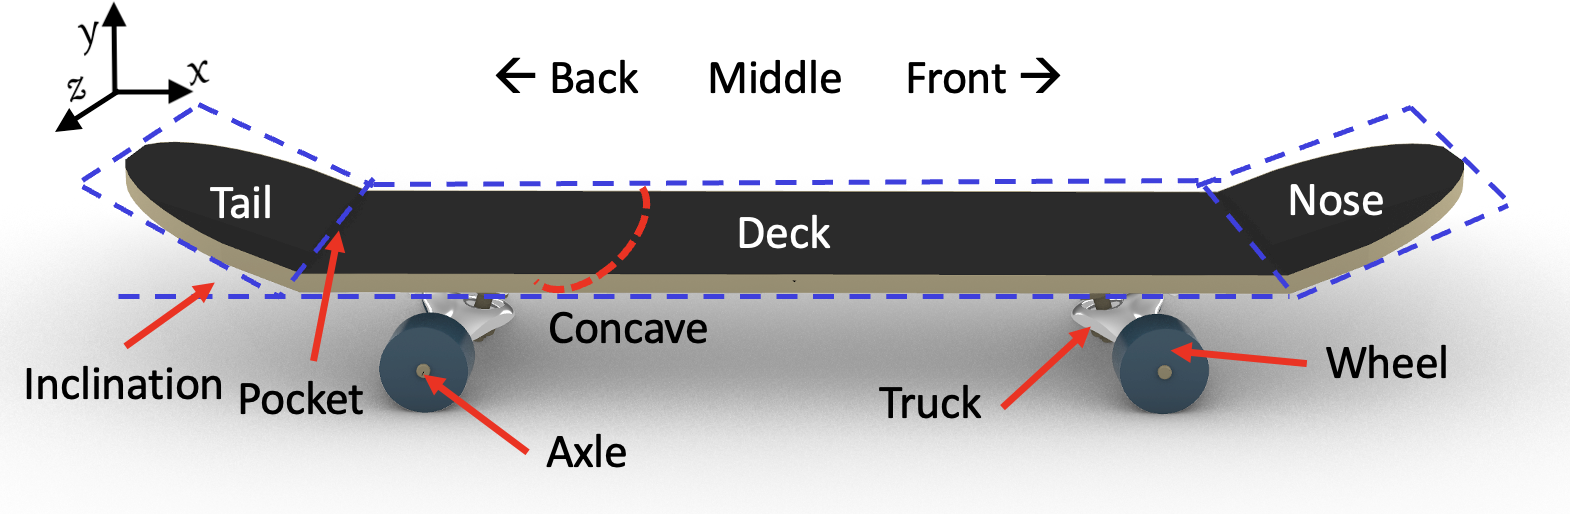
\includegraphics[width=0.5\textwidth]{figure/terminology.png}
    \caption[Skateboard terminology]{Skateboard terminology}
    \label{fig:skateboard terminology}
\end{figure}

\subsection{Mechanics of the ollie} \label{ss_mechanics}
Figure~\ref{fig:ollie steps} details 11 motion cues ($t_1-t_{11}$) observed during an ollie, found by analysing a slow-motion video.

Friction occurs between the feet and the grip-tape due to the force normal to the board exerted by the feet together with sliding movement tangential to the surface.
This benefits ollie height because the resultant force (figure~\ref{fig:ollie steps} $t_5$, blue arrow) is directed more vertically upwards than the normal force (figure~\ref{fig:ollie steps} $t_4$, green arrow), which results in less downward motion while leveling out the skateboard mid air.
The higher the coefficient of friction between the foot and the deck, the more upward the resultant force will be.
That is why grip-tape on the deck and rubber-soled shoes is the choice of preference among skaters (coefficient of friction of 0.7 or higher~\cite{bron_nog_nodate}).

\section{Method}
% I have parameterized the geometry and inertia characteristics of a skateboard modeled as a single rigid body with parameters: tail length, tail angle, deck length, truck height, and wheel radius. This is an appropriate parameterization for a skateboard designer because the width of the skateboard is usually chosen by preference. Also, the ollie is a movement that involves rotation in one plane, visible in fig. \ref{fig:ollie steps}, which means only the inertia characteristics for this rotation are necessary. 

To find the optimal skateboard geometry, we take a modeling and optimization approach involving four fundamental steps: 
\begin{enumerate}
    \item understand the mechanics of the ollie through literature and a video analysis,
    \item define the parameter optimization and \gls{ocp},
    \item implement the mechanics into the optimization problem, and
    \item solve the optimization problem.
\end{enumerate}

\subsection{Geometry and Parameterization}\label{s_paropt}
The most widely used modern skateboard is the popsicle stick skateboard. We simplify the popsicle stick skateboard design for our 2D model with an assumption about nose-tail symmetry and by ignoring the deck concavity, and describe it with ten variables, see Table~\ref{t_variables}. The variables colored blue in Figure~\ref{f_11segments} are optimized and the green variables are set to an industrial standard because they influence the mass and inertia properties but play little role in the ollie dynamics.
%
\begin{table}
  \centering
  \begin{tabular}{=l +l +c}
    \toprule
    \rowstyle{\textbf}& Variable & Description \\
    \midrule
    \rowstyle{\color{blue}} & $l_{wb}$ & Wheelbase \\
    \rowstyle{\color{blue}} & $l_{d}$ & Deck length \\
    \rowstyle{\color{blue}} & $l_{t}$ & Tail/nose length \\
    \rowstyle{\color{blue}} & $\phi$ & Tail/nose inclination \\
    \rowstyle{\color{blue}} & $h_{tr}$ & Truck height \\
    \rowstyle{\color{blue}} & $r_{w}$ & Wheel radius \\
    \rowstyle{\color{ao}} & $h_d$ & Deck thickness \\
    \rowstyle{\color{ao}} & $d_{tr}$ & Truck width \\
    \rowstyle{\color{ao}} & $d_{d}$ & Deck width \\
    \rowstyle{\color{ao}} & $d_w$ & Wheel width \\
    \rowstyle{\color{orange}} & $d_{com}$ & COM distance from deck \\
    \bottomrule
  \end{tabular}
  \caption{Variables used to describe skateboard shape (see fig.
    \ref{f_11segments}). Blue parameters are optimized, green parameters are
    set to industrial standard. Orange is a dependent on other variables.}
  \label{t_variables}
\end{table}

%%%%%%%%%%%%%%%% begin figure %%%%%%%%%%%%%%%%%%%
\begin{figure}
  \centerline{
    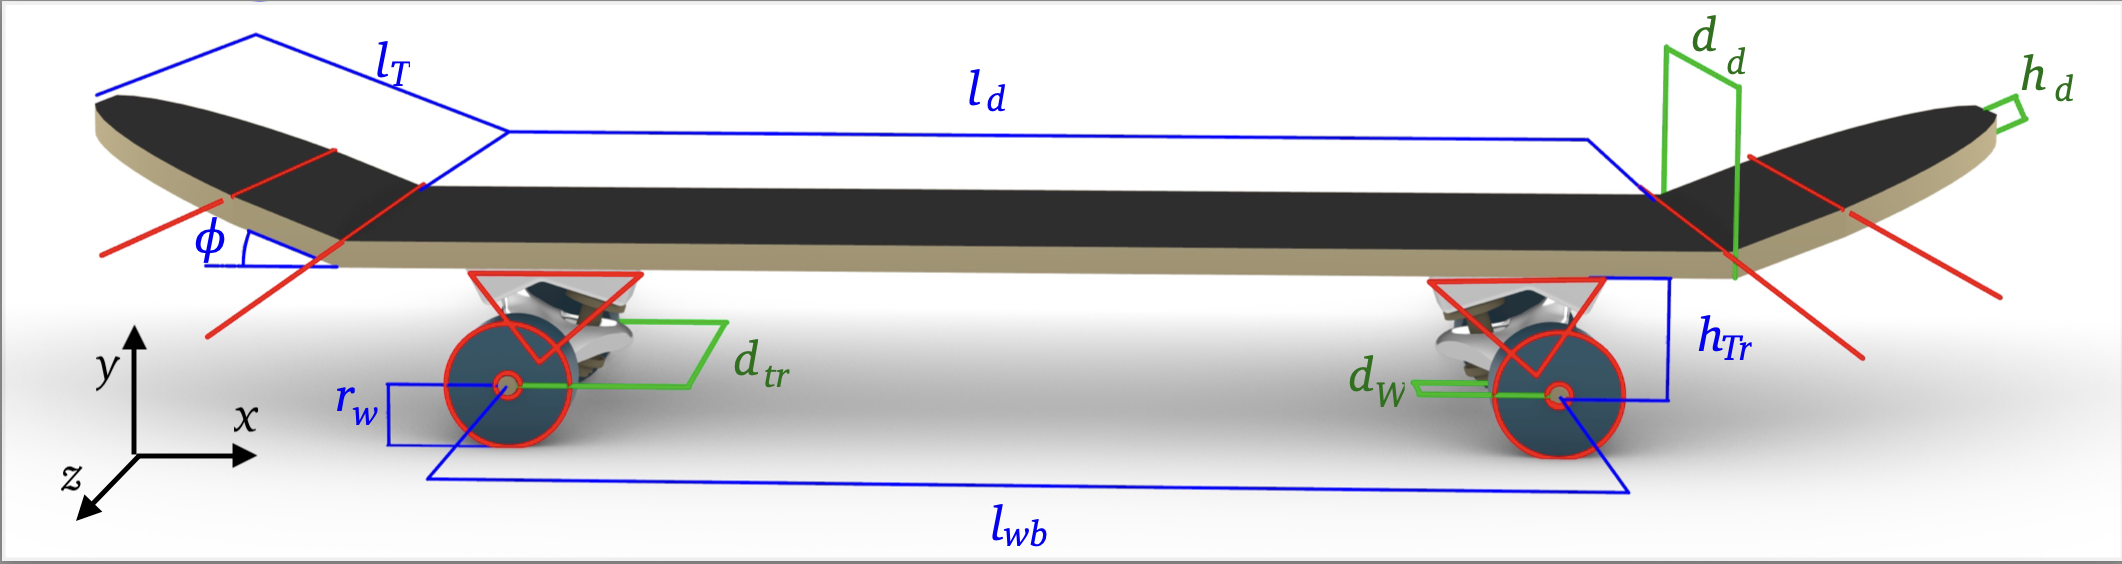
\includegraphics[width=0.5\textwidth,trim={0.1cm 0.1cm 0.1cm 0.05cm},clip]{figure/parameterized.png}
  }
  \caption[11-Segment skateboard model]{Parameterized skateboard. Red lines
    split the skateboard into 11 basic shaped segments for inertia calculation
    (see figure \ref{f_basicshapes})}
\label{f_11segments}
\end{figure}
%%%%%%%%%%%%%%%% end figure %%%%%%%%%%%%%%%%%%%

We developed a mass and inertial model, which is a function of the skateboard's essential geometry, see Figure~\ref{f_11segments}), and material densities (wood, steel, urethane). The model is made up of eleven basic constant density shapes shown in Figure~\ref{f_basicshapes}: semi-cylinders, cuboids, cylinders and triangular prisms.
%
\begin{figure}
  \centering
  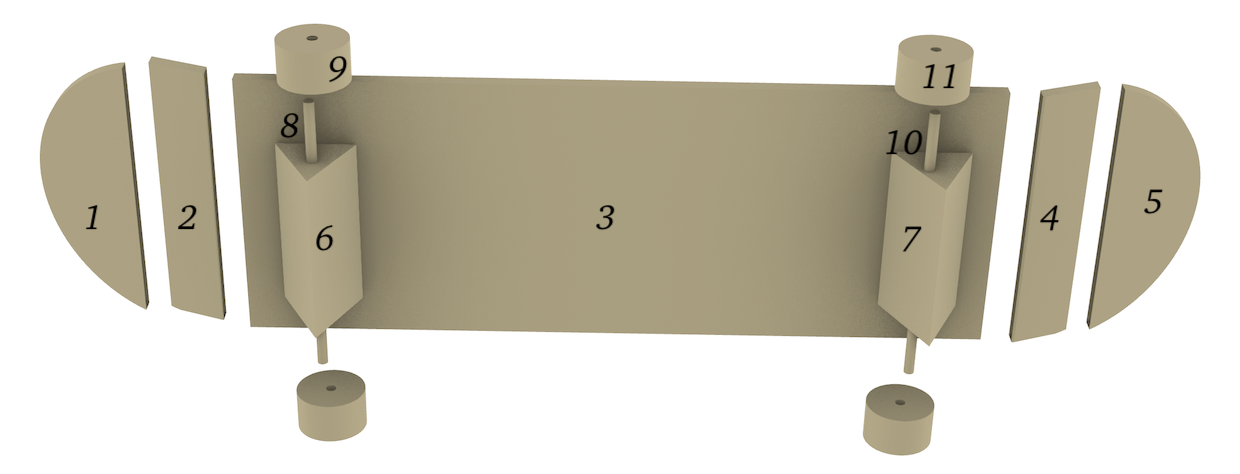
\includegraphics[width = 0.5 \textwidth]{figure/Basicshapes.png}
  \caption[Exploded 11 segment model]{Clarification on the 11 segment model.
    13 shapes are visible, but the wheels are taken as one wider cylinder in
    2D. Sections 1-5 are wood, 6, 7, 8, 10 are steel, and 9, 11 are urethane.}
  \label{f_basicshapes}
\end{figure}

\subsection{Optimal Control Problem}
We formulate an \gls{ocp} with the objective of maximising the peak board height during the ollie. This is a simultaneous trajectory optimization of the board's dynamics and control, and parameter optimization of its geometric parameters. We use a direct method as they are well-suited for when dynamics and control must be computed to a similar accuracy and the structure of the control trajectory is not known a priori~\cite{kelly_introduction_2017}. We make use of Pycollo~\cite{brockie_2021_predictive} to numerically solve the \gls{ocp}. Pycollo solves the generalized multi-phase \gls{ocp} described in \cite{betts_2010_practical} by transcribing the \gls{ocp} to a \gls{nlp} using an LGL (Legendre-Gauss-Lobatto) collocation method~\cite{betts_2016_using}. The \gls{nlp} is then solved using Ipopt~\cite{biegler_2009_large}. Pycollo also uses ph-mesh refinement~\cite{patterson_2015_ph} to iteratively improve the transcription mesh, solving successive \glspl{nlp} until a desired solution tolerance is met.

\subsection{Phases and Objective} \label{s_phases}

We use a multi-phase formulation for the ollie \gls{ocp} to handle discontinuities in the state trajectories in a numerically-stable manner. The allows, for example, the impact of the tail with the ground during the pop to be treated as an impulse, which is not possible during a single continuous phase. A disadvantage of this approach however is that the transition between phases is prescribed, leaving no room for the optimizer to discover these transitions. The three dynamically-distinct phases are:
\begin{enumerate} \label{n_phases}
  \item Preparation phase
  \item Upward motion
  \item Downward motion
\end{enumerate}

During the preparation phase the back wheels are in contact with the ground. The tail impact with the ground defines the transition from preparation to the upward motion. During upward and downward motion nothing is in contact with the ground and they both are governed by the same \glspl{eom}. We split the upward motion and downward motion into two phases because Pycollo requires that the objective function be a function of initial or final state variables of a phase~\cite{brockie_2021_predictive}. The transition from upward to downward motion defines the highest ollie.

To  define the maximum height achieved during the ollie, we constrain the board to be level at the highest point and
take the height achieved to be the middle of a fictional tangent touching lowest point of both wheels. The objective function for maximization is:
%
\begin{equation}
  \mathcal{J} = y_s^{(2)}(t_F) + d_{com} - h_{tr} - r_w
\end{equation}

\noindent where $y_s^{(2)}(t_F)$ is the height achieved by the skateboard's \gls{com} at the end of the second phase, $d_{com}$ is the distance between the skateboard's \gls{com} and the deck, $h_{tr}$ is the truck height, and $r_w$ is the wheel radius.

\subsection{System Dynamics}\label{s_systemdynamics}

\subsubsection{Skateboard Equations of Motion}
While in reality a skateboard bends and flexes during the ollie, this study assumes a rigid body model of the skateboard to reduce mathematical complexity.

The skateboard model is detailed in figure~\ref{fig:FBD}. In phase 1 we use a sliding joint for the rear wheel contact to eliminate the ground reaction forces from the \glspl{eom}.
During phase 2 and 3 the skateboard is an unconstrained rigid body in 2D. 

We derive the \glspl{eom} using the TMT method~\cite{vallery_heike_advanced_2018}, facilitated by SymPy~\cite{meurer_sympy_2017}.
The code used for the derivation is provided in the supplementary information, along with a mathematical description of the \glspl{eom}.

\begin{figure}
    \centering
    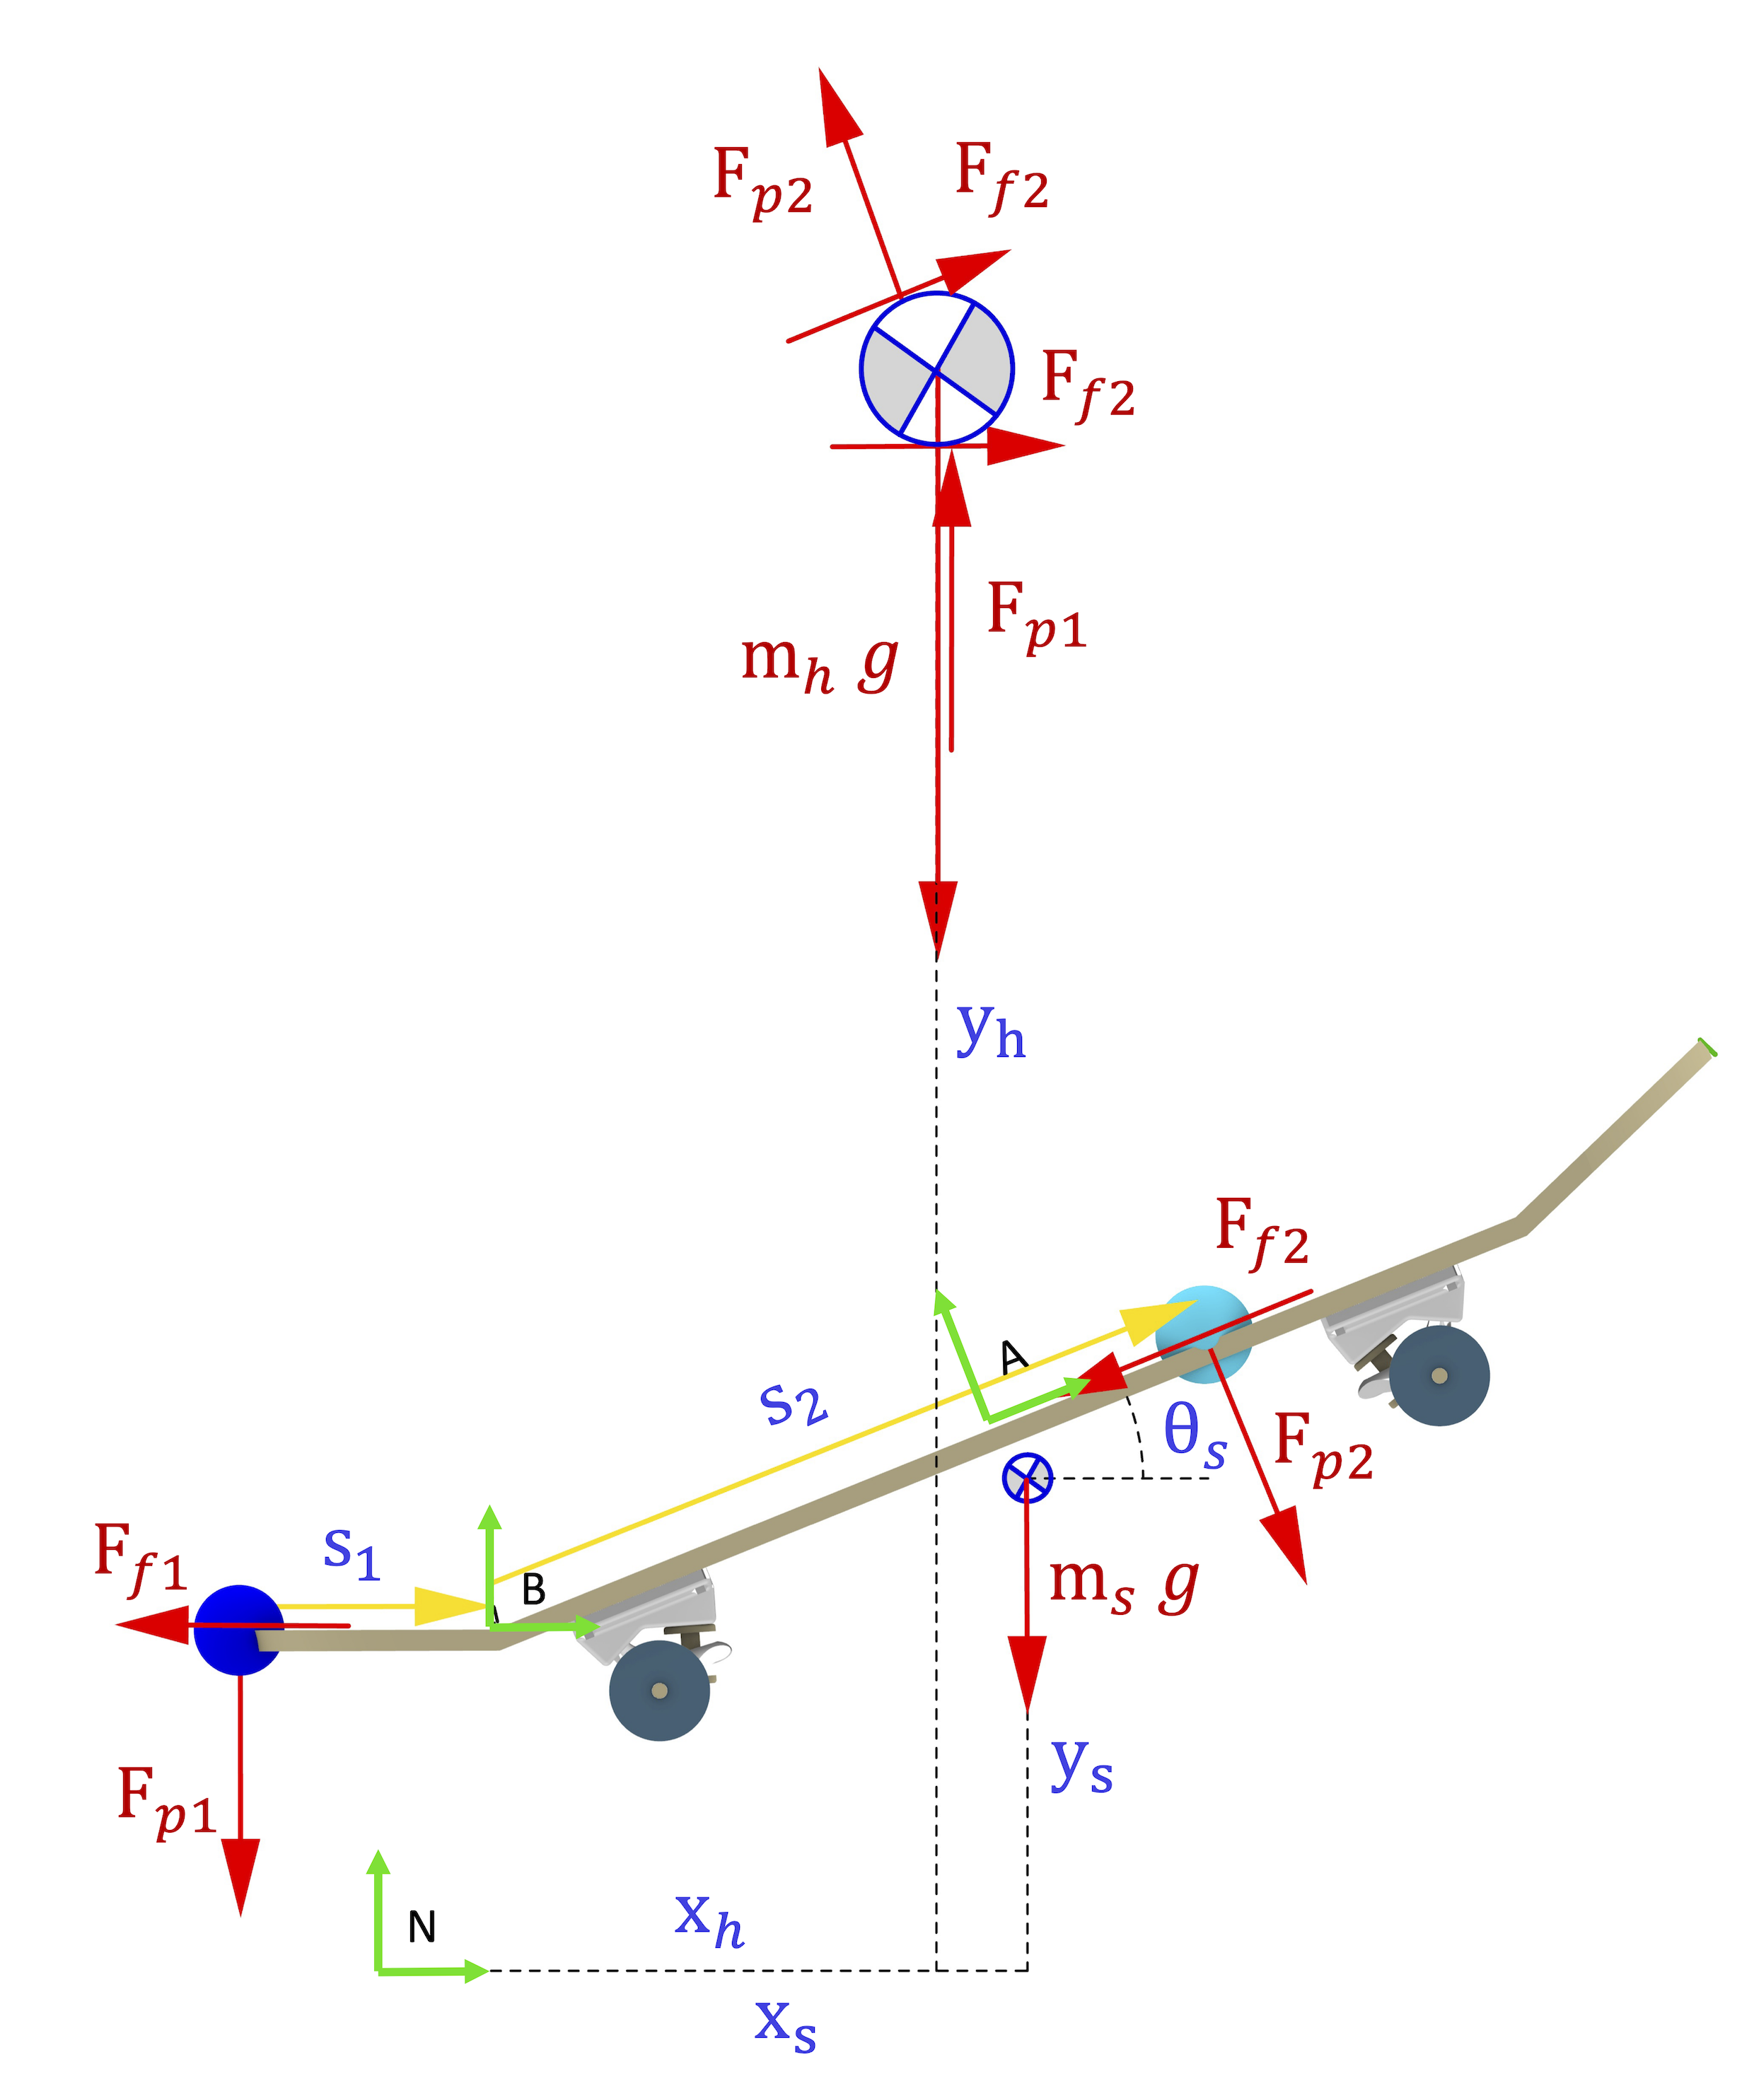
\includegraphics[width=0.45\textwidth]{figure/FBD_skater_feet.png}
    \footnotesize\begin{tabular}{|l l|l l|} \hline
    \color{blue}Blue: & State variables &\color{red} Red: & Forces \\ \hline
    \color{cyan}Cyan dot: & Front foot & \color{blue}Blue dot: & Back foot \\ \hline
    \color{yellow}Yellow: & Foot movement & \color{green}Green: & Frames \\ \hline
    \end{tabular}
    \caption[Free Body Diagrams phase 2 and 3]{Free body diagrams of human and skateboard for phase 1. $N$ is the inertial frame, and $A$ and $B$ are body fixed frames. Forces acting between the feet and human's \gls{com} are equal and opposite.}
    \label{fig:FBD}
\end{figure}

\subsubsection{Human Equations of Motion}
The human is represented by a point mass on top of the skateboard, again detailed in figure~\ref{fig:FBD}.
The interactions between the point mass and the skateboard are modeled as a pair of equal and opposite forces acting between the massless feet and the human's \gls{com}.
Due to this simplification, this model is not represent metabolic leg power, only the mechanical power output~\cite{van_der_kruk_power_2018,morin_biomechanics_2018}. Inertia of the human's body segments is neglected.

The code used to derive to \glspl{eom} of the human, along with a mathematical description, can again be found in the supplementary information.

\subsection{Constraints}

\subsubsection{Human Model}

We constrain the kinetics and kinematics of the human to compensate for the simplifications used.

Musculoskeletal restrictions bound the kinematics of the human controller.
Firstly, the feet can only operate within a fixed region relative to the human's \gls{com}.
We found this region's bounds using Yeadon \cite{yeadon_simulation_1990} by scaling the model to a \SI{1.80}{\meter} tall human and posing it to match a picture of Jake Hayes' world record ollie (figure~\ref{fig:f_record}). 

\begin{figure}
    \centering
    \subfloat[\centering 45.5" world record ollie. $^{1}$  ]{{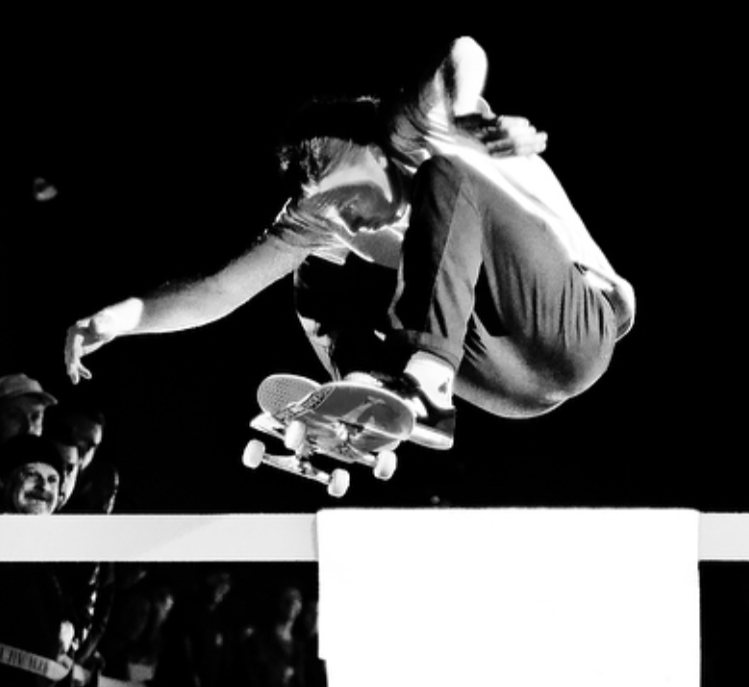
\includegraphics[width=0.2\textwidth]{figure/JakeHayes.png} }}%
    \quad
    \subfloat[\centering Yeadon model in same configuration]{{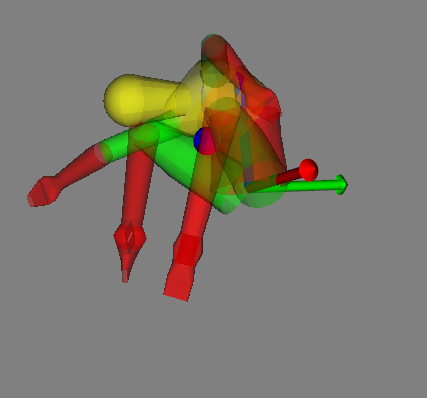
\includegraphics[width=0.2\textwidth]{figure/JakeHayesYeadon.png} }}%
    \caption{Reconstruction of world record ollie} 
    \label{fig:f_record}
    \centering \footnotesize \url{https://theberrics.com/world-record-ollie-footage}$^{1}$%
\end{figure}

We also implement a minimum and maximum foot separation of \SI{0.1}{\meter} and \SI{1.0}{\meter} respectively, along with constraining the skater to always stay on top of the skateboard to eliminate relative errors.
To make sure the feet never leave the skateboard, $s_1$ and $s_2$ are positively bound from the end of the tail and the left pocket of the deck respectively (see fig \ref{fig:FBD}).
The feet can still be in a no contact scenario, as seen in section~\ref{ss_mechanics}, due to how the friction model is implemented (section~\ref{ss_friction}).

The human kinetics are bounded to the characteristics of a \gls{cmj} during the first phase of the ollie.
The \gls{cmj} motion is chosen because it accounts for 76.3\% of the variance in the performance of the ollie~\cite{candotti_lower_2012} and is a reliable assessor of lower-body mechanical power~\cite{barker_relationships_2018}.
During a vertical jump, joint torques, and knee extensor and hip abduction forces all map to one output variable: the \gls{grf}.
As contributions of individual segments cannot be expressed with a point mass model, we bound the \gls{grf} of the \gls{cmj} to capture the realistic kinetics of the human. The \gls{grf} for a representative \gls{cmj} is shown in figure~\ref{fig:cmj}.

\begin{figure}
    \centering
    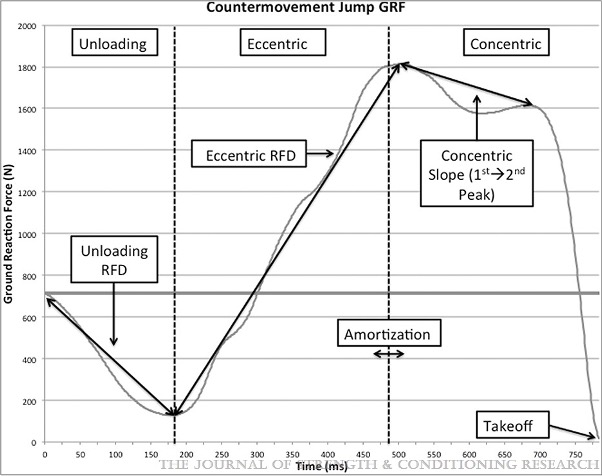
\includegraphics[width=0.45\textwidth]{figure/countermovementjumpRFD.jpg}
    \caption[Ground reaction force of \acrlong{cmj}]{Phases during \gls{cmj}. During unloading, the human lowers their \gls{com} quickly. During the eccentric phase, the gained downward velocity during the unloading phase is braked until the lowest point is reached which is at the amortization. During the concentric phase the legs are stretched out and upward speed is gained until the take-off. At take-off the vertical speed is maximal.}
    \centering \footnotesize Source: \cite{barker_relationships_2018}%
    \label{fig:cmj}
\end{figure}

We constrain the \gls{rfd} to simulate the leg shortening and lengthening cycle, the maximum force $F_{max}$ keep this within realistic limits, and maximum mechanical power $P = F v_{rel}$ as this also constrains velocity. We derived numerical values from a study that tested Division-I male soccer players with a mean height of \SI{179.5}{\centi\meter}, weight of \SI{75.5}{\kilo\gram}, and age of 19.65 years~\cite{barker_relationships_2018}. To account for the fact that \cite{barker_relationships_2018} measured two legs simultaneously, we also constrain the sum of the forces produced by both legs together, as well as the absolute force and power produced by each legs to within realistic physical limits.

\subsubsection{Friction Model} \label{ss_friction}
In section \ref{ss_mechanics}, we show that the feet slide along the deck's
griptape to level the skateboard out during the preparation phase 1 and drag
the skateboard up during the upward motion phase 2.
We use both static and dynamic friction to model the foot sliding across the
deck's surface and make use of the relaxed friction formulation presented by
Patel et al.~\cite{patel_contact-implicit_2019} to do so.
This method allows for unplanned discontinuous frictional contact with direct
collocation without needing a hybrid method.
Usually this would be considered impossible since direct collocation enforces
the dynamics and constraints over a continuous domain, where discontinuities in
the system dynamics usually lead to infeasibility
\cite{kelly_transcription_2017}.
The downside is that it is difficult to converge to a feasible solution without
a close initial guess and the computation time can be higher
\cite{shield_contact-implicit_2022,patel_contact-implicit_2019}.
We simplified Patel et al.'s method by removing the impact condition between
the human and the board.
We assume that the feet never impact the skateboard and simply exert zero
normal force when out of contact.
We can do this because, unlike Patel et al., we do not model the human as
multiple body segments but as a point mass.
Patel et al. requires the initial guess to be similar to the solution, and the
model 43 minutes to solve \cite{shield_contact-implicit_2022}. Our model solves
optimally under two minutes with an initial guess of zero.

We start by setting the normal forces of the feet $F_{p1},F_{p2}$ and the feet
accelerations as control variables.
The acceleration is controlled instead of the foot location itself to ensure
have smooth realistic foot trajectories.
Our control variables are:
%
\begin{equation}
    \mathbf{u}^{(1,2,3)} = [F_{p1},F_{p2},\ddot s_1, \ddot s_2]
\end{equation}

We utilize the remainder of Patel's friction approach for the foot sliding and
the tail hitting the ground. We consider both static and Coulomb friction when
in motion.
The friction is solved with a set of constraints.
Here we derive the friction of the back foot along the skateboard; the front
foot friction is obtained by exactly the same process.
The first step to implement friction is to create slack variables that divide
the friction forces $F_{f1},F_{f2}$ into a positive and negative components:
%
\begin{equation} \label{e_plusminfric}
   F_{f1} = F_{f1}^+ - F_{f1}^-
\end{equation}

As described in section \ref{s_systemdynamics}, the forces perpendicular to the
skateboard are positive definite such that the force can never pull on the
skateboard. Now the created slack variables also need to be positive definite:

\begin{equation}
    F_{p1} \geq 0,\quad F_{f1}^+ \geq 0,\quad F_{f1}^- \geq 0
\end{equation}

The magnitude of dynamic friction is $F_{p1}\ \mu$ with a direction opposed to
the relative sliding velocity.
The static friction is bound by the yellow surface of the friction cone in fig.
\ref{f_frictioncone} and is only possible when the feet are not sliding.
To realize this, another slack variable $\psi$ is introduced which represents
the magnitude of the relative velocity $\dot s_1$ between the foot and the
skateboard.
%
\begin{equation}
\begin{split}
    \gamma_{18}^{(1,2,3)}: \quad & \psi_1 + \dot s_1  \geq 0 \\
    \gamma_{19}^{(1,2,3)}: \quad & \psi_1 - \dot s_1  \geq 0 \\
\end{split}
\end{equation}

Now static friction can be implemented with a set of constraints:

\begin{equation}
\begin{split}\label{e_frictioncontrol}
       \gamma_{20}^{(1,2,3)}: \quad & \mu F_{p1} - F_{f1}^+ - F_{f1}^- \geq 0 \\
       \gamma_{21}^{(1,2,3)}: \quad & (\mu F_{p1} - F_{f1}^+ - F_{f1}^-)\ \psi_1  = 0
\end{split}
\end{equation}

The first constraint assures that the positive or negative component of the
friction is always smaller than $\mu F_{p1}$. The second constraint ensures
that when the foot slides ($\psi_1 \not = 0$),  the sum of the positive and
negative friction components equal $\mu F_{p1}$. It is important that when
sliding in positive direction, the negative friction component $F_{f1}^-$
should equal $\mu F_{p1}$ and $F_{f1}^+=0$ and vice versa. This is realized
with the following constraints:

\begin{equation}
\begin{split}
    \gamma_{22}^{(1,2,3)}: \quad & F_{f1}^+ (\psi_1 + \dot s_1)  = 0 \\
    \gamma_{23}^{(1,2,3)}: \quad & F_{f1}^- (\psi_1 - \dot s_1)  = 0
\end{split}
\end{equation}

This type of constraint ($A\cdot B = 0$) has three possible solutions $A= 0,\
B=0,\ or\ A,B = 0$. By filling in a numerical example, the desired behaviour is
shown. For example looking at the first constraint, when $\dot s_1 = -1$, then
$\psi_1 + \dot s =  0$ and $F_{f1}^+$ can be a positive number. Then looking at
the second constraint, when $\dot s = -1$, then $\psi - \dot s = 2$ and
$F_{f1}^- = 0$. Combining this with the second equation in equation
\ref{e_frictioncontrol} gives: $(\mu F_{p1} - F_{f1}^+ - 0) \cdot 0 = 0$, which
results in $F_{f1}^+ = \mu F_{p1}$. This is exactly what it should be given a
negative relative sliding velocity. The friction for the front foot adds
another six constraints: $\gamma_{24-30}^{(1,2,3)}$

\subsubsection{Endpoint constraints} \label{p_endpoints}
To fully describe the ollie optimization problem, all phases need to be glued together. In the multi-phase optimization scheme all initial and final time variables are treated as separate variables. By constraining the corresponding variables between the phases, the variables can be treated as one variable over all three phases: 

\begin{equation}
    \begin{array}{c}
         \beta_1: \quad t_F^{(1)} = t_0^{(2)}  \\
         \beta_2: \quad t_F^{(2)} = t_0^{(3)}  \\
    \end{array}
\end{equation}

To know the phase switching instance, the optimization should switch phase when hitting the tail to the ground. This is implemented by calculating the impact angle of the skateboard as a function of the parameter values:

\begin{equation}
    \theta_{impact} = -\operatorname{atan}\left(\frac{h_{t r}+l_t \sin (\phi)+r_w}{-\frac{l_d}{2}-l_t \cos (\phi)+\frac{l_{w b}}{2}}\right)
\end{equation}

Which is implemented as an endpoint constraint as:

\begin{equation}
    \beta_3: \quad \theta_s^{1}(t_F) = \theta_{impact}
\end{equation}

During this collision the ground exerts a normal linear impulse normal. To calculated speeds after impact, we used a matrix representation method of the Newton impact law\cite{vallery_heike_advanced_2018}:

\begin{equation}
\begin{array}{l c}
    \beta_{4,5,6,7}: & \left[\begin{array}{cc}
        \mathbf{M_s} & \mathbf{C_{c,i}} \\
        \mathbf{C_{c,i}}^T & 0
    \end{array} \right]\
    \left[\begin{array}{c}
       \mathbf{\dot q}^{(2)}(t_0)  \\
        \rho_c 
    \end{array}\right] =
     \\ &  
     \left[\begin{array}{c}
         \mathbf{M_s}\ \mathbf{\dot q}^{(1)}(t_F)   \\
         -e\ \mathbf{C_{c,i}}^T\ \mathbf{\dot q}^{(1)}(t_F)
    \end{array}\right]
    \end{array}
\end{equation}

Where $\dot q_{rel}^{(2)}(t_0)$, and $\dot q_{rel}^{(1)}(t_F)$ are the relative speeds just after impact at the first collocation point of phase 2, and just before impact at the last collocation point of phase 1 respectively.  $e$, the empirical constant related to the amount of dissipated energy during impact, is the coefficient of restitution (COR) with $e=1$ resulting in mechanical energy preservation, and for $e=0$ all energy is dissipated. $C_{c,i}$ is the constraint equation describing contact. Lastly, $\rho_c$ is a Langrange multiplier to solve the reaction impulse.

Because the states in phase 1 are expressed in different variables than phase 2 as shown in section \ref{s_systemdynamics}, variables $\dot q^{(1)}(t_F)$ are rewritten to the CoM coordinates $x_s,y_s$, and $\theta_s$. Also the initial values of variables $x_s^{(2)}(t_0), y_s^{(2)}(t_0)$ are dependant on the final time variables $x_w^{(1)}(t_F), \theta_s^{(1)}(t_F)$ and are set as an endpoint constraint

\begin{equation}
\begin{array}{l c c}
\beta_8: \ x_s^{(2)}(t_0) & = & \frac{l_{w b} \cos \left(\theta_s\right)}{2}+x_w^{(1)}(t_F)- \\ 
& & \left(-d_{c o m}+h_{t r}\right) \sin \left(\theta_s^{(1)}(t_F)\right) \\

\beta_9: y_s^{(2)}(t_0) & = & \frac{l_{w b} \sin \left(\theta_s\right)}{2}+r_w+ \\ 
& & \left(-d_{c o m}+h_{t r}\right) \cos \left(\theta_s^{(1)}(t_F)\right)
\end{array}
\end{equation}

To make sure the human starts the ollie from a standing position, the vertical forces at the beginning of phase 1 are equal to the body-weight:

\begin{equation}
    \beta_10: \quad \mathbf{F_h} \cdot \mathbf{\hat n_y} = m_h g
\end{equation}

The definition of landing the ollie has been set to the back wheel touching the ground at a minimum of 0 [rad] (level) and a maximum of $\frac{1}{6} \pi$[rad] (rotated counter clockwise). The optimization stops when the back wheel touches the ground.

\begin{equation}
\begin{array}{l c}
\beta_11 : & \frac{-l_{wb}}{2} \sin(\theta_s(t_F^{(2)})) - r_w + y_s(t_F^{(2)}) + \\ 
& (d_{com} - {d_tr}) \cos(\theta_s(t_F^{(2)}))
\end{array}
\end{equation}

Variables $\theta_s, s_1, s_2, \dot s_1, \dot s_2, x_h, y_h, \dot x_h, \dot y_h$ have equal endpoints between phase 1 and 2 ($b_{12-21})$. All state variables have equal endpoints between phase 2 and 3 ($b_{21-35}$). Initial and final endpoint constraints are set to a wide range and are found in Appendix B.

\subsection{Settings}\label{s_settings}
The NLP tolerance is set to $1e^{-8}$, and the mesh tolerance is set to $1e^{-3}$. The amount of mesh sections for the first two phases are set to 30, phase 3 is set to 10 mesh sections. The landing phase is not as important as the preparation and upward motion phase as those define the final height and thus the objective.

\subsection{Summary}\label{s_summary}
To summarize all the findings, the general formula for the multi-phase ollie OCP is implemented in one overview. The objective function for the ollie OCP is 

\begin{equation}
     maximize\ (y_s^{(2)}(t_F) + d_{com} - h_{tr} - r_w)
\end{equation} 

Subject to the dynamical constraints in phase 1:

\begin{equation}
\begin{array}{c}
        \alpha_{1} = \frac{\mathbf{F_h}\cdot \mathbf{\hat n_x}}{m_h}\\
        \alpha_{2} = \frac{\mathbf{F_h}\cdot \mathbf{\hat n_y}}{m_h}\\
        \alpha_{3,4}^{(1)} =   \left(\mathbf{T}^T \mathbf{M_s} \mathbf{T} \cdot  \mathbf{T}^T\right)^{-1} (\mathbf{F_a} - \mathbf{M_s} \cdot \mathbf{g_k})
\end{array}
\end{equation}

And for phase 2 and 3:

\begin{equation}
    \begin{array}{c}
        \alpha_{1} = \frac{\mathbf{F_h}\cdot \mathbf{\hat n_x}}{m_h}\\
        \alpha_{2} = \frac{\mathbf{F_h}\cdot \mathbf{\hat n_y}}{m_h}\\ 
        \alpha_{5,6} = (\mathbf{M_s})^{-1}\mathbf{F_a}
    \end{array}
\end{equation}

With path constraints during phase 1:

\begin{equation}
    \begin{array}{c}
         \gamma_{3-6},  \\
         \gamma_{9-30},
    \end{array}
\end{equation}

And during phase 2 and 3:

\begin{equation}
    \begin{array}{c}
         \gamma_{1-11}  \\
         \gamma_{16-30}
    \end{array}
\end{equation}

With endpoint constraints $\beta_{1-9}$.
In the first phase the state variables $q^{(1)}$, control variables $u_c^{(1)}$, slack control variables $u_s^{(1)}$ are:

\begin{equation}
\begin{array}{rl}
   \mathbf{q^{(1)}} =& [x_w , th_s, x_h, y_h, \dot x_w, \dot th_s,\dot x_h, \dot y_h]    \\
   \mathbf{u_c^{(1)}} =& [fp1, fp2, dds_1, dds_2]  \\
   \mathbf{u_s^{(1)}}=&  [F_{f1}^+, F_{f1}^-, \psi_1,F_{f2}^+, F_{f2}^-, \psi_2 
\end{array}
\end{equation}

During the second and third phase the state variables $q^{(2,3)}$, control variables $u_c^{(2,3)}$, slack control variables $u_s^{(2,3)}$ are:

\begin{equation}
\begin{array}{rl}
   \mathbf{q^{(2,3)}} =& [x_s, y_s, \theta_s, x_h, y_h, \dot x_s, \dot y_s, \dot \theta_s,\dot x_h, \dot y_h]    \\
   \mathbf{u_c^{(2,3)}} =& [F_{p1}, F_{p2}, \ddot s_1, \ddot s_2]  \\
   \mathbf{u_s^{(2,3)}}=&  [F_{f1}^+, F_{f1}^-, \psi_1,F_{f2}^+, F_{f2}^-, \psi_2] 
\end{array}
\end{equation}

With the global parameters variables $\sigma$ as any combination of the optimized geometric parameters: 

\begin{equation}
    \sigma_i \in [l_{wb}, l_d, l_t, \phi, h_{tr}, r_w]
\end{equation}

The results will show several optimizations with different combinations of parameter optimizations to search the solution space for optimal shapes. The first set of optimizations will be without optimized parameter variables to show proper functioning of the model. The second set of optimizations will be single variable optimizations where only one variable from the optimized parameter variables is chosen to be optimized. The third set of optimization will be variations to multiple optimized parameter variables. 

%%%%%%%%%%%%%%%%%%%%%%%%%%%%%%%%%%%%%%%%%%%%%%%%%%%%%%%%%%%%%%%%%%%%%%
\section{Results}
Figures \ref{f_singlepar}, and \ref{f_multipar} show 9 skateboard shapes that have improved ollie height compared to the industrial standard popsicle stick skateboard geometry (Base in figure \ref{f_nopar}) when optimized for optimal ollie height. The best performing skateboard shape (number 2 in figure \ref{f_multipar} improved ollie height by 11.1 \%. All optimizations are with a null seed initial guess and solved with an optimal IPOPT exit status with the desired NLP tolerance and mesh tolerance found in \ref{s_settings}. All optimizations were solved within 3 minutes. Four skateboards did not show improvement in ollie height, which are indicated with a red dot in figures \ref{f_singlepar}, \ref{f_multipar}. These are per definition local maxima, because the base optimization provides a higher solution, which is in the solution space of these optimizations. 

\subsection{Optimal Trajectories and \\Geometries}
\subsubsection{No parameter optimization}
\begin{figure*}
    \centering
    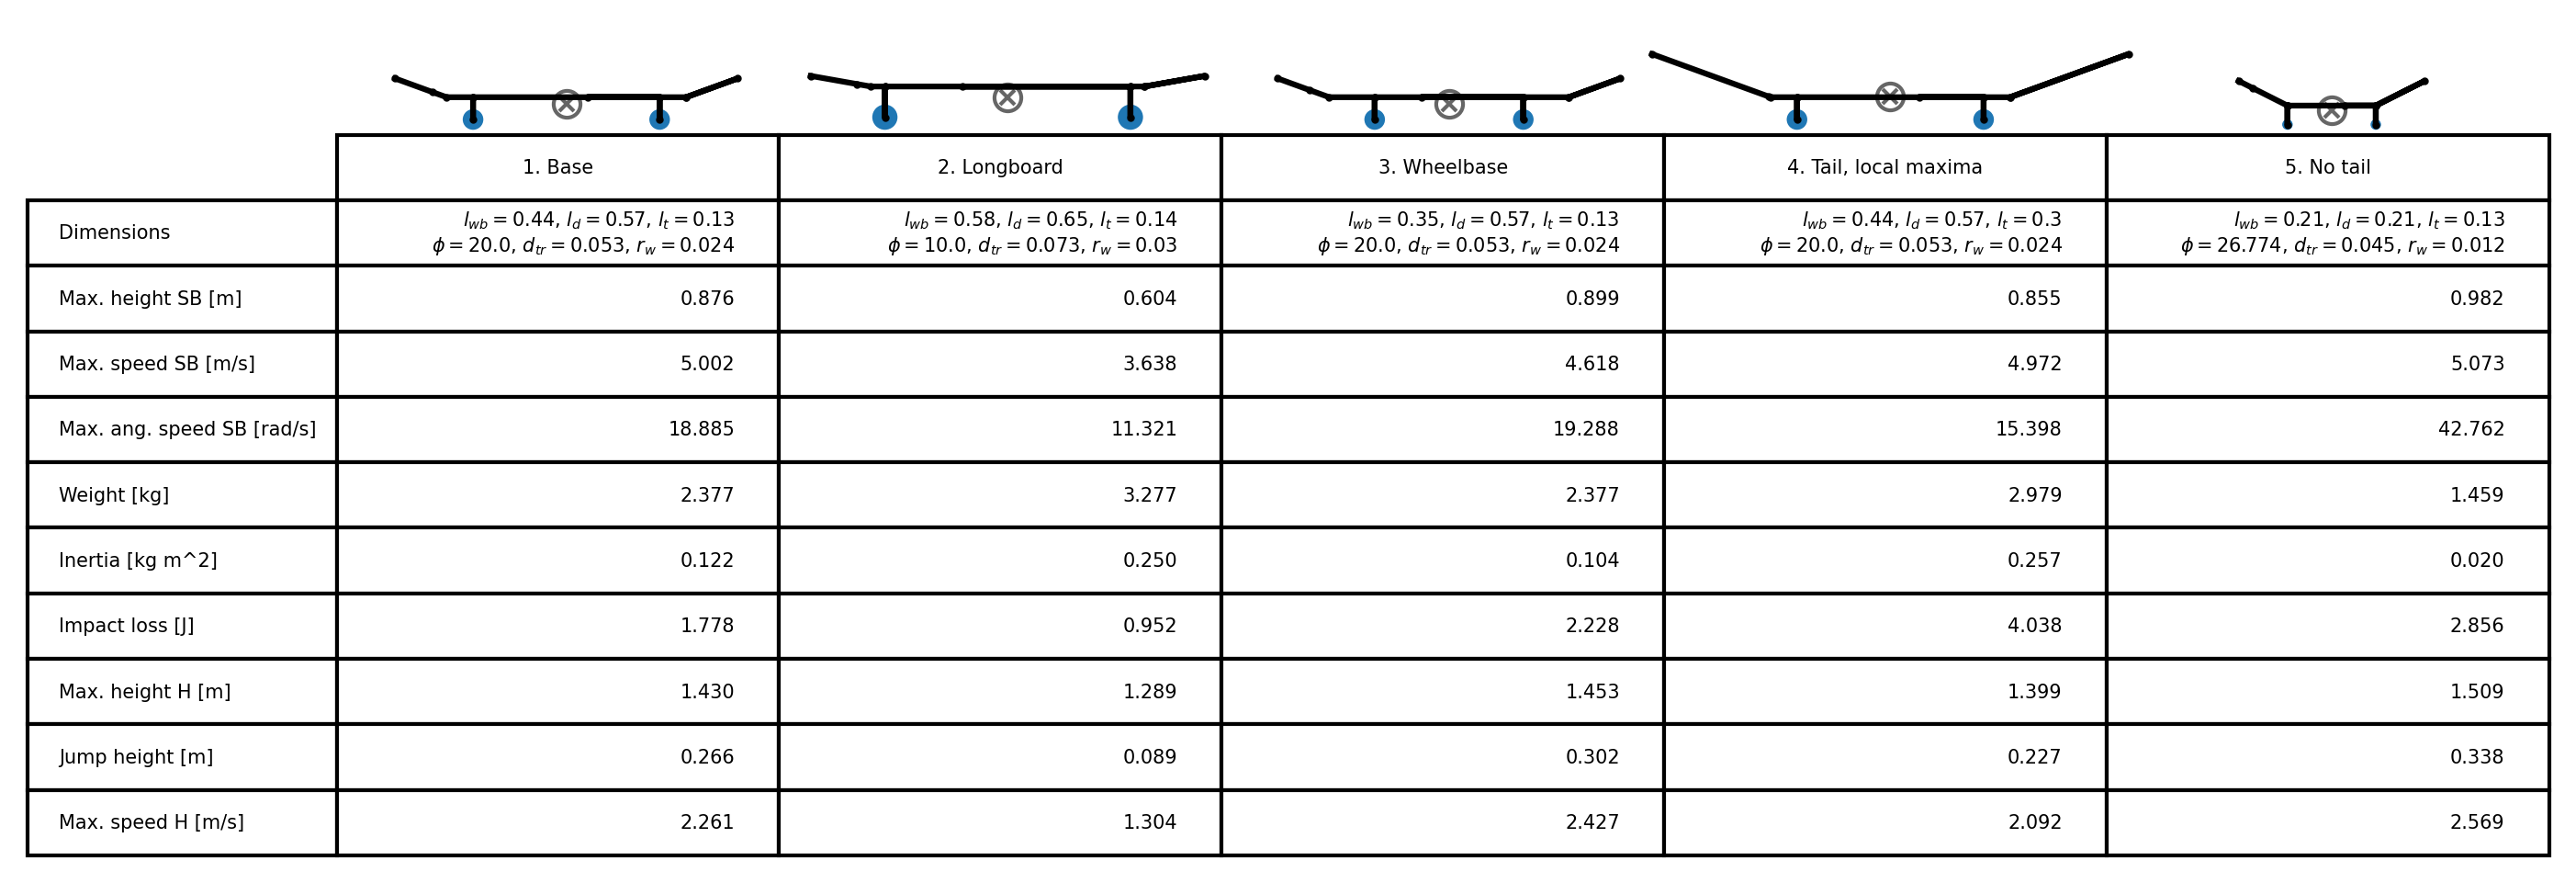
\includegraphics[width=\textwidth]{paper/figure/Results/ResultsTable.png}
    \caption[Results benchmarks]{5 Different ollie optimization results showing important benchmarks. 1, and 2 are without parameter optimization. 2 is conducted to verify reality (long board should be harder to ollie). 3, and 4 are trajectory optimizations with single parameter optimization, the optimized parameter is indicated with the name. 4 is a local maximum since the base optimization can ollie higher and is in the solution space of 4. 5 is a trajectory optimization with multiple parameter optimization, where all parameters are optimized but the tail length (causes local maxima).}
    \label{fig:enter-label}
\end{figure*}
% \begin{figure*}[!t]
% \captionsetup[subfigure]{}
%     \subfloat[4 solutions without parameter optimization. The solutions are the result of different industry standard skateboards to verify that the optimization matches reality.]{
%     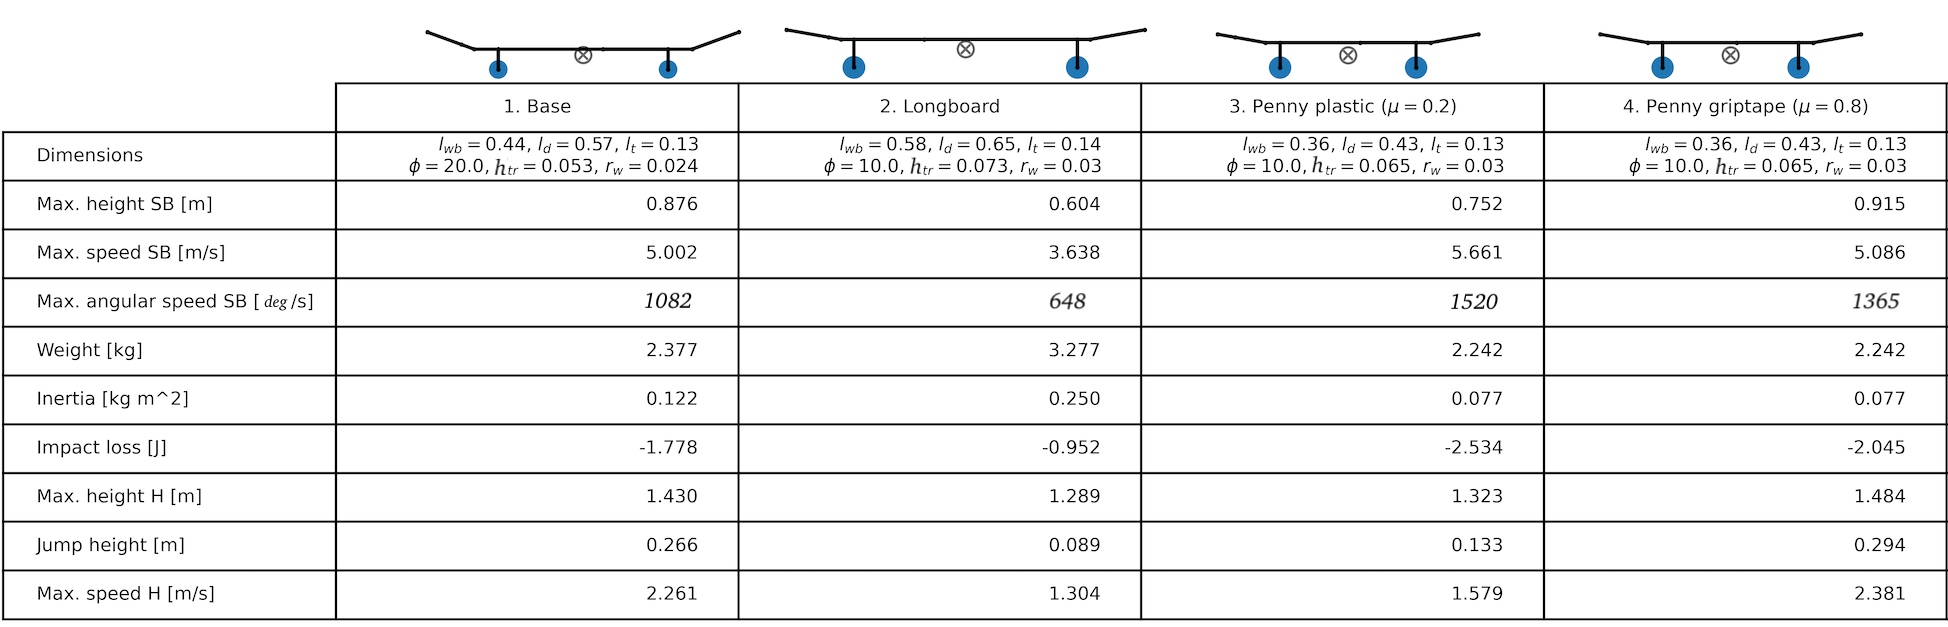
\includegraphics[trim={0 0 0 0},clip,width=\textwidth]{figure/Results/no_optimization_table_dpi600.png}
%     \label{f_nopar}}

%     \subfloat[6 solutions whilst optimizing a single parameter. 5 and 6 are local maxima since they perform worse then 1. Base in (a) (base solution is in solution space of 5 and 6). The best performing optimization is 2. Wheelbase]{
%         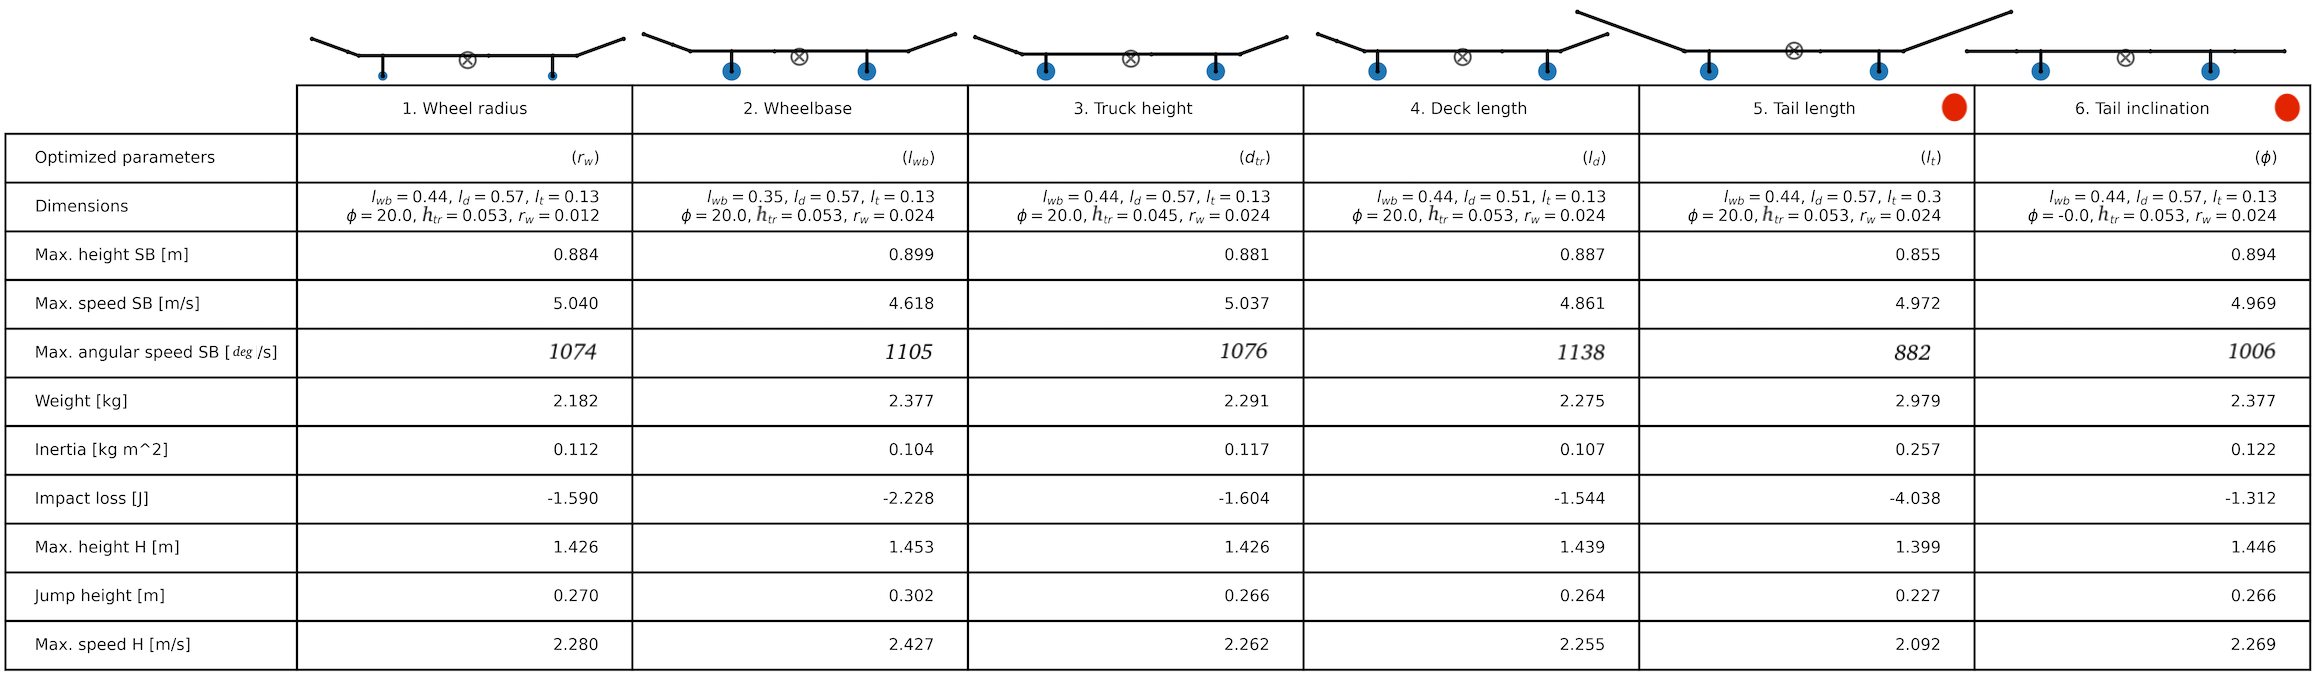
\includegraphics[trim={0cm 0cm 0cm 0cm},clip,width=\textwidth]{figure/Results/single_optimization_table_dpi600.png}
%         \label{f_singlepar}
%        }
       
%     \subfloat[5 solutions whilst optimizing multiple parameters. 3 and 5 are local maxima since they perform worse then solution 1. ]{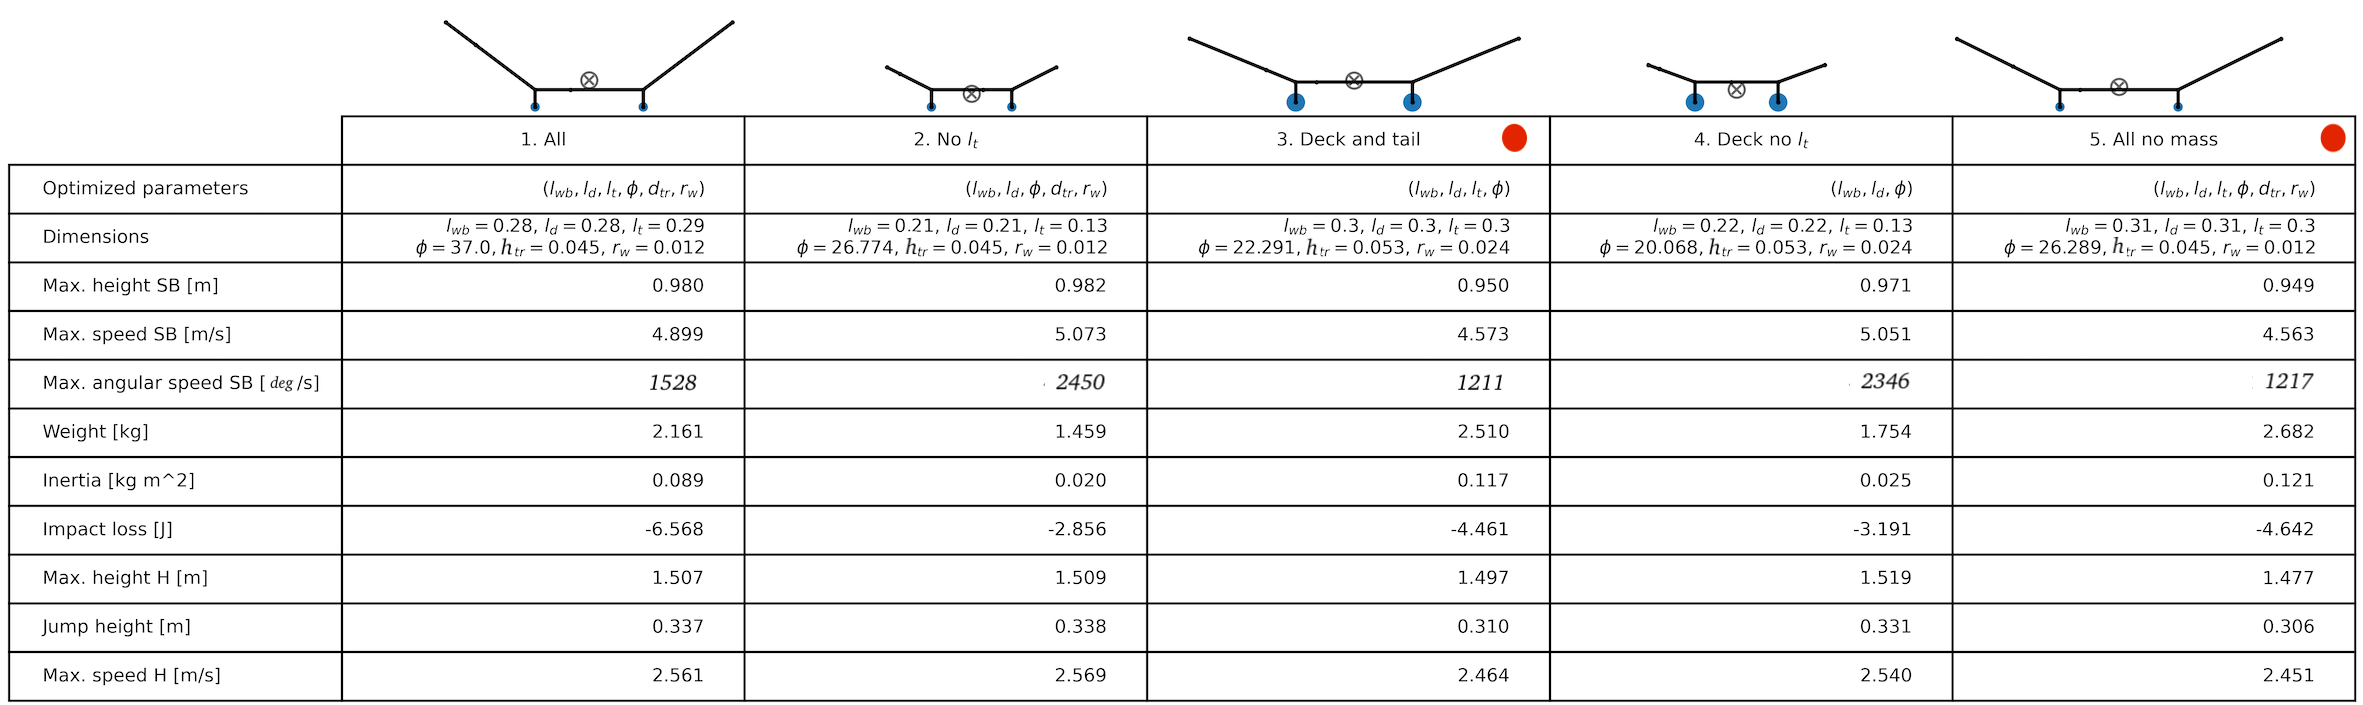
\includegraphics[trim={0cm 0cm 0cm 0cm},clip,width=\textwidth]{figure/Results/multi_optimize_table_dpi600.png}\label{f_multipar}}
%     \vspace{0.2cm}
%     \caption[Geometries of optimization solutions]{Results of 3 optimization types}
%     a): No parameter optimization, (b) Single parameter optimization, (c) Multiple parameter optimization. The columns show different solutions with a schematic geometry on top. The rows show corresponding optimal control benchmarks. The centre of mass is indicated with a cross. Jump height is calculated by minimum vertical position minus take-off vertical position of the person. The impact loss is calculated with kinetic energy of the skateboard after impact minus kinetic energy of the skateboard prior to impact. Other variables are direct output from optimization.
% \end{figure*}

\noindent The results in figure \ref{f_nopar} are performed to test the scenario that a long board and a penny board are more difficult to ollie compared to the popsicle stick. These results are found without a parameter optimization. The longboards' dimension are set to an arbitrary OEM longboard.\footnote{\url{https://hlcskateboardfactory.com/ shape: MB701}} The penny boards' dimensions are set to an arbitrary penny board. A penny board is usually made from plastic.\footnote{\url{https://skateboardelite.com/what-is-penny-board/}} The coefficient of friction for the plastic penny is set to 0.2 \cite{bani-hani_data_2019}. For a comparison if the shape of a penny could actually ollie higher a version with grip-tape is also shown. The three boards are optimized to verify the optimization. Longboard complies with the real life scenario and the optimization shows a 31\% decrease in ollie height compared to the base . The penny board with a plastic top (lower coefficient of friction) is able to ollie 14.2\% lower than the base.

The base skateboard is able to ollie 31\% higher than the long board. The longboards' maximum angular velocity is 40.0\% lower compared to the base skateboard. This is probably due to the fact that the inertia and mass of the long board are higher which will make it harder for the human with limited power to rotate it and get it up. The jump height of the human on the long board is 66.5\% lower compared to the base, meaning that a lot of power is going into the long board instead of jumping up. Resulting in the human mainly to tuck in without jumping). The impact loss is lower for the long board. This could be correlated to the fact that it reaches lower speeds. The contrary is seen with the plastic penny board. It reaches higher speeds and loses more energy during impact. The penny boards are 5.7\% lighter than the base board but have a lower inertia mainly due to the smaller size of the penny board. With a plastic penny board, the human is not able to ollie higher than with the base skateboard. The human jumps 50.0\% and ollies 0.124 [m] lower with the plastic penny board. With grip-tape the penny board is able to ollie higher than the base skateboard. In real life the penny board and long board are harder to ollie. The same is shown in the optimization for the long board. This suggests that the kinetics of the optimization are similar to reality. The penny with grip-tape is able to ollie higher than the base skateboard, which could have multiple causes. One of them is that a real penny board is made of plastic which deforms more than wood. Which causes more dissipation of energy and a more difficult control to ollie. The other cause could be that the optimization is lacking kinematic constraints for the human. In real life it is harder to maintain balance when your feet are in a narrow stance. During the balancing narrow stance, in real life it could be more difficult to exert maximal leg power.

\subsubsection{Single parameter optimization}

\noindent The results in figure \ref{f_singlepar} are found with a single parameter optimization. Compared to the base skateboard, all single parameter optimization skateboards were able to ollie higher except for the tail length optimization. The difference in ollie height between the base and the single parameter optimizations is minimal (0.05-0.023 [m]) which suggests that the base skateboard is very close to it's optimum when only one variable can be changed. All single parameter skateboards except for the wheelbase and tail length optimizations show similar human jump height. Which indicates that with these configurations the human is able to exert similar power over time. With a smaller wheelbase the human was able to jump higher. The main differences are found in the weight and inertia reduction which could be the main `drive' of the single parameter optimization. Geometrically the optimizer isn't able to find a large ollie improvement as seen between the base and long board. Still, the optimizer can find a higher optimum by decreasing weight and inertia with all single parameter optimizations except for the tail length and tail inclination optimizations. Which indicates that inertia and weight reduction is a positive influence for ollie height. Dynamically this makes sense because with lower mass and inertia values it easier to lift and rotate the skateboard. The wheel radius, truck height, and tail inclination are hitting the bounds of 0.0125[m], 0.045[m], and 0[deg] respectively, which may indicate a local maxima. Also the tail length optimization did not find a higher maxima than the base optimization which makes it a local maximum per definition, because the base skateboard is a possible solution for this optimization.

\subsubsection{Multiple parameter optimization}

\noindent The results in figure \ref{f_multipar} are found with multiple parameter optimization. When multiple parameters are optimized the ollie height is improved by 0.074-0.106 [m] compared to the base skateboard. The first column, 'All' in figure \ref{f_multipar} shows the set-up when all parameters are optimized. As seen with the single parameter optimization the tail length is causing strange optima. Once again it is shown that when not optimizing the tail length, the ollie height is higher. This proves that the optimization of all variables is a local optimum, since the optimum found with the `no $l_t$' (figure \ref{f_multipar}) skateboard is a possible solution to the optimization. Same goes for the full deck optimization. The full deck optimization does not optimize wheel radius and truck height. The ollie height for this optimization is 0.021 [m] lower than the same optimization with fixed tail length. This proves that the full deck optimization is a local maxima which is caused by the optimization of the tail length. The cause of hitting a local optimum because of the tail length needs further investigation. When the tail length increases the impact loss increases as well. This is logical when thinking of the tail speed $v = \omega \times r$, which means, the larger the distance between the tip of the tail and COM of the skateboard, the larger the local speed at the tail. The larger the speed at the tail, the more momentum is lost during impact, which is the reason for the higher impact losses. The impact loss is dependant on the mass and speed, the higher the mass or the speed, the higher the impact loss will be. For example in the `no $l_t$' (figure \ref{f_multipar}) optimization the angular velocity before impact is more than twice as high compared to the base optimization. But the mass is also 0,878[kg] less. Thus, the large angular velocity causes the impact loss to be higher, but the mass reduction reduces it, only causing a slight gain in impact loss. 

The most promising optimizations are analyzed further by looking into the states and control over time and compared to the base optimization. The single parameter optimizations show little improvement. The best performing single parameter optimization is the wheelbase optimization with an increase of 2.6\%. The best performing multiple parameter optimization are `no $l_t$' (figure \ref{f_multipar}) (12.0\% increase in ollie height) and deck without tail length (10.7\% increase in ollie height).  All other detailed figures of the optimizations are found in Appendix A. 
\begin{figure*}
    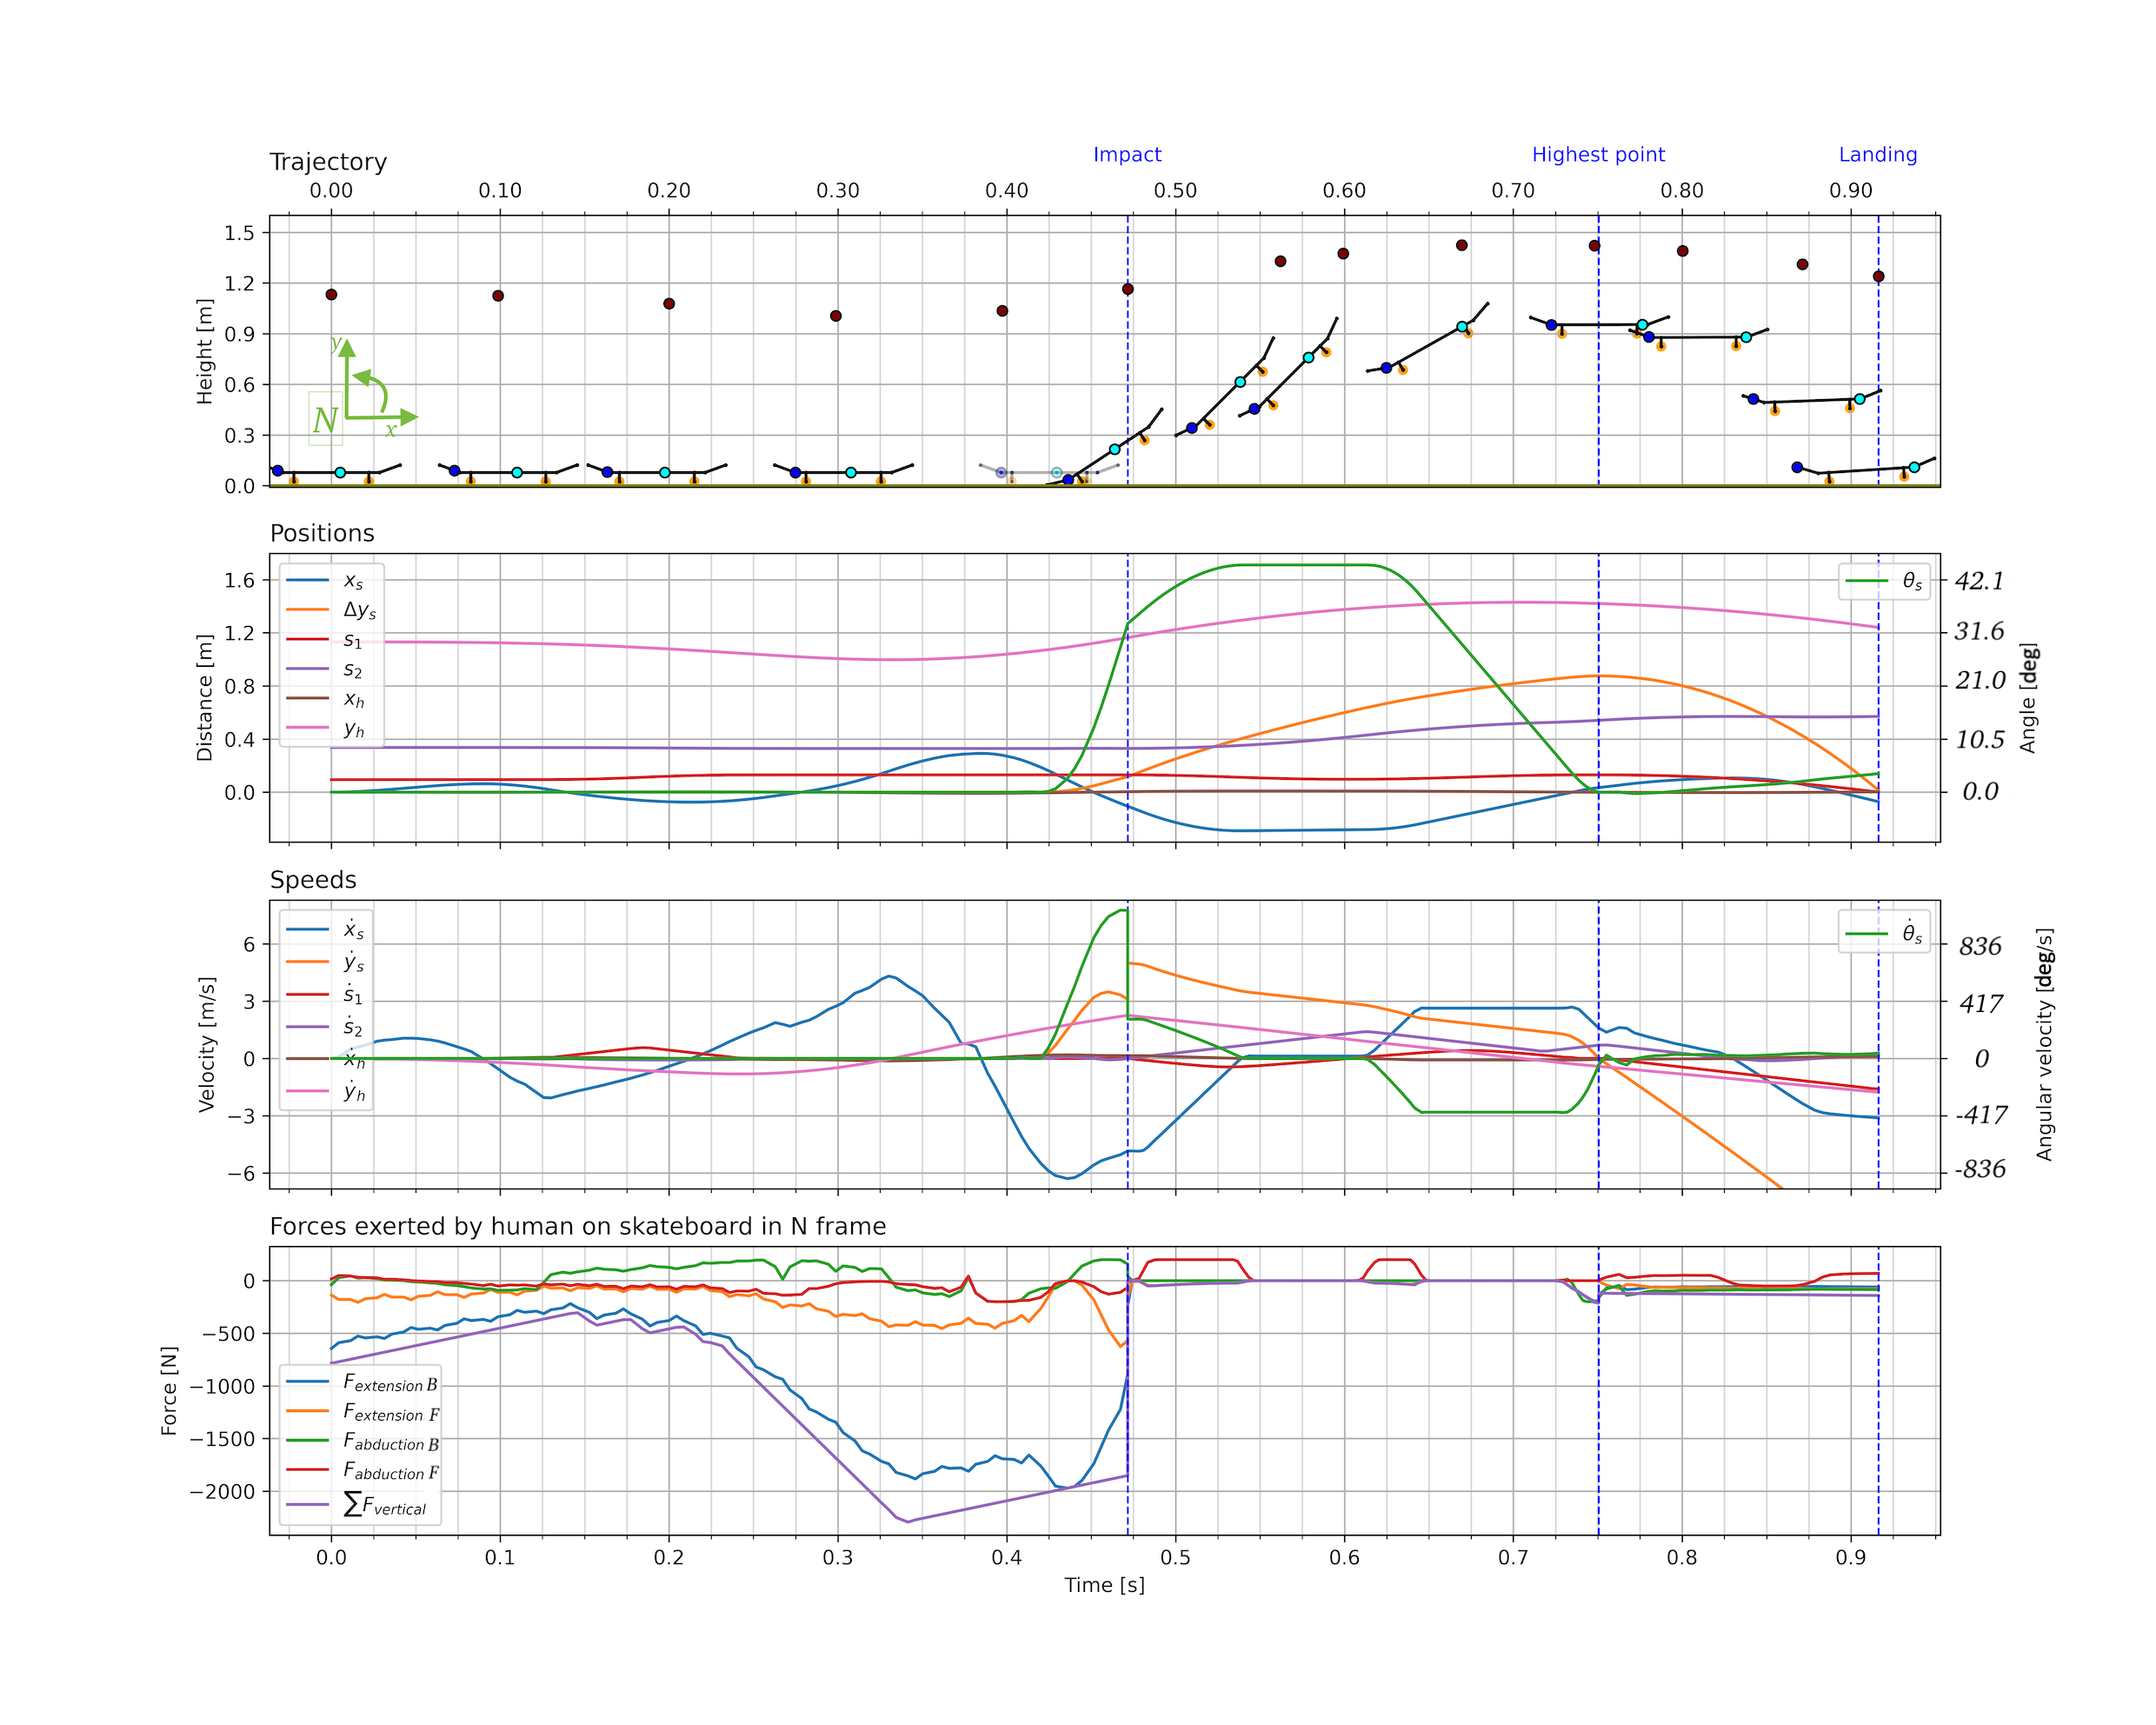
\includegraphics[trim={0cm 0cm 0cm 0cm},clip,width=\textwidth]{figure/Results/data_basedpi600.png}
    \vspace{-1.5cm}\caption[Trajectory, positions, speeds, and forces of base optimization]{
    Detailed trajectory of base skateboard}\label{f_noparameter}
    Graph (1) shows the trajectory of the skateboard, the COM of the human corresponds to the time. (2) are the coordinates of the skateboard and the human over time. (3) are the speeds of skateboard and human over time. (4) are the extension (N-frame y direction - see first plot for frame convention), abduction (N-frame x direction) and sum of extension forces. The blue dotted lines are the phase switches. First the human lowers their COM (pink,2) by decreasing vertical force (purple, 4), at minimal human COM height there is maximal force and zero speed (pink,3). Maximal force is almost fully caused by the extension force of the back foot (blue,4). Speed is increased until impact and it reaches maximum speed (pink,3 at impact). Just before impact the skateboard rotates its angle (green,2) from 0 to impact angle. Mid air the speeds are constant except ones effected by gravity (orange,pink,3). The moments forces are exerted the velocities change (t=0.5, t=0.63). The human reaches its highest point before the skateboard. At the highest point force is exerted to `catch' the skateboard. Landing is achieved by stretching and landing on the back wheel.
    
\end{figure*}
\subsection{Detailed trajectories}
To see all detailed trajectories with forces as a video, visit: \url{https://www.youtube.com/watch?v=jw5DmNnvD7c}.

\subsubsection{Base skateboard optimization}

%%% Maybe we should try to fit this subsubsection in the caption of figure 11 %%%
\noindent The first figure concerns the optimal control problem without parameter optimization shown in figure \ref{f_noparameter}. The trajectory is very similar to the trajectory seen in figure \ref{fig:ollie steps}. Though you have to take into account that this ollie is a standing ollie without an initial horizontal velocity, whereas figure \ref{fig:ollie steps} shows a riding ollie. The skateboard relative to the human first moves forward, and just before the impact it rapidly moves backward followed by the tail hitting the ground. The backwards movement happens such that the human can effectively pull the skateboard up and forward with friction and perpendicular force which results in the skateboard being straight under the human at the highest point. The backwards velocity is clearly visible in fig. \ref{f_nopar} speeds, where the blue line before impact is at the largest negative velocity. After impact the velocity will gradually become positive and ending at an almost 0 x position of the skateboard (blue line in positions at second dotted line). If there would not have been a backwards movement, the skateboard would have been pushed out of reach of the human's feet when the board is leveling out. The skateboard is leveled out by a positive abduction force of the front foot (red line forces at $t=0.47-0.55$ and $t=0.62-0.65$). These forces result in a decrease in angular rotation (green line speeds, same time span), and a level skateboard at the highest point (green line positions at highest point = 0).
You can see that the back foot is almost fully located at the pocket of the skateboard. This is the point with the lowest velocity of the tail, the tip of the tail has the highest velocity due to $v = \omega \times r$. When the board is rotating the power that can maximally be exerted by the human legs is limited by the force and the relative velocity: $P_{leg} = v_{rel} F$. This means that if the intention is to jump up as high as possible, the relative speed should be as low as possible, which is why the foot should be in the pocket. When the foot would be on the tip, more distance is lost which could have resulted in a higher jump. 
The impact changes the momentum of the skateboard. In the speeds graph it is visible that the angular velocity at impact vastly reduces (green line, 1082 to 286 [deg/s]), whilst vertical velocity is gained (orange line, 3 to 5 m/s).
The human starts with their knees slightly bent, and having full body weight on the skateboard. In the first phase the human lowers their COM in order to prepare the legs to jump. This is called the unloading phase (from $t=0 - 0.2$). After the unloading phase the force increases. Here the human is braking the downward velocity gained during the unloading phase up until the highest peak of the sum of the vertical forces (purple line). This is called eccentric braking. Then the human vertical velocity (pink line speeds) is at 0 and the human has reached its lowest point. From $t=0.35$ until impact the human is gaining upward speed  (pink line speeds) and reducing the force. The force needs to reduce to comply to the power bound ($P_{leg} = v_{rel} F$). This phase is called the concentric phase. Then the human has lost contact from the skateboard just after impact. Followed by an upward motion gradually decreasing due to gravity, reaching it's highest point just before the skateboard reaches it's highest point. The slopes and maximum of the vertical forces (purple line) are bound by the eccentric RFD(negative) and concentric RFD(positive) and the maximum force permitted. The optimizer is at the bounds and wants to maximize force and power output. The forces are not fully smooth due to the fact that the bounds are on both legs, thus simultaneous counteracting of forces between the front and back leg is permitted in the optimization. Having more kinetic data on single legs could improve this. Also the polynomial to estimate the solution used by the software is not plotted correctly here, so the line should be smoother when using the polynomials used per mesh section provided by the software. Due to practical implications this has not been done. The third reason why the control can be less? smooth is due to the friction constraints. These constraints are difficult to solve and are demanding for the optimizer, which sometimes results in non-smooth forces.
The landing is slightly on the back wheels and the human is almost fully stretched out when landing.

\subsubsection{Wheelbase optimization}
\begin{figure*}
    \centering
    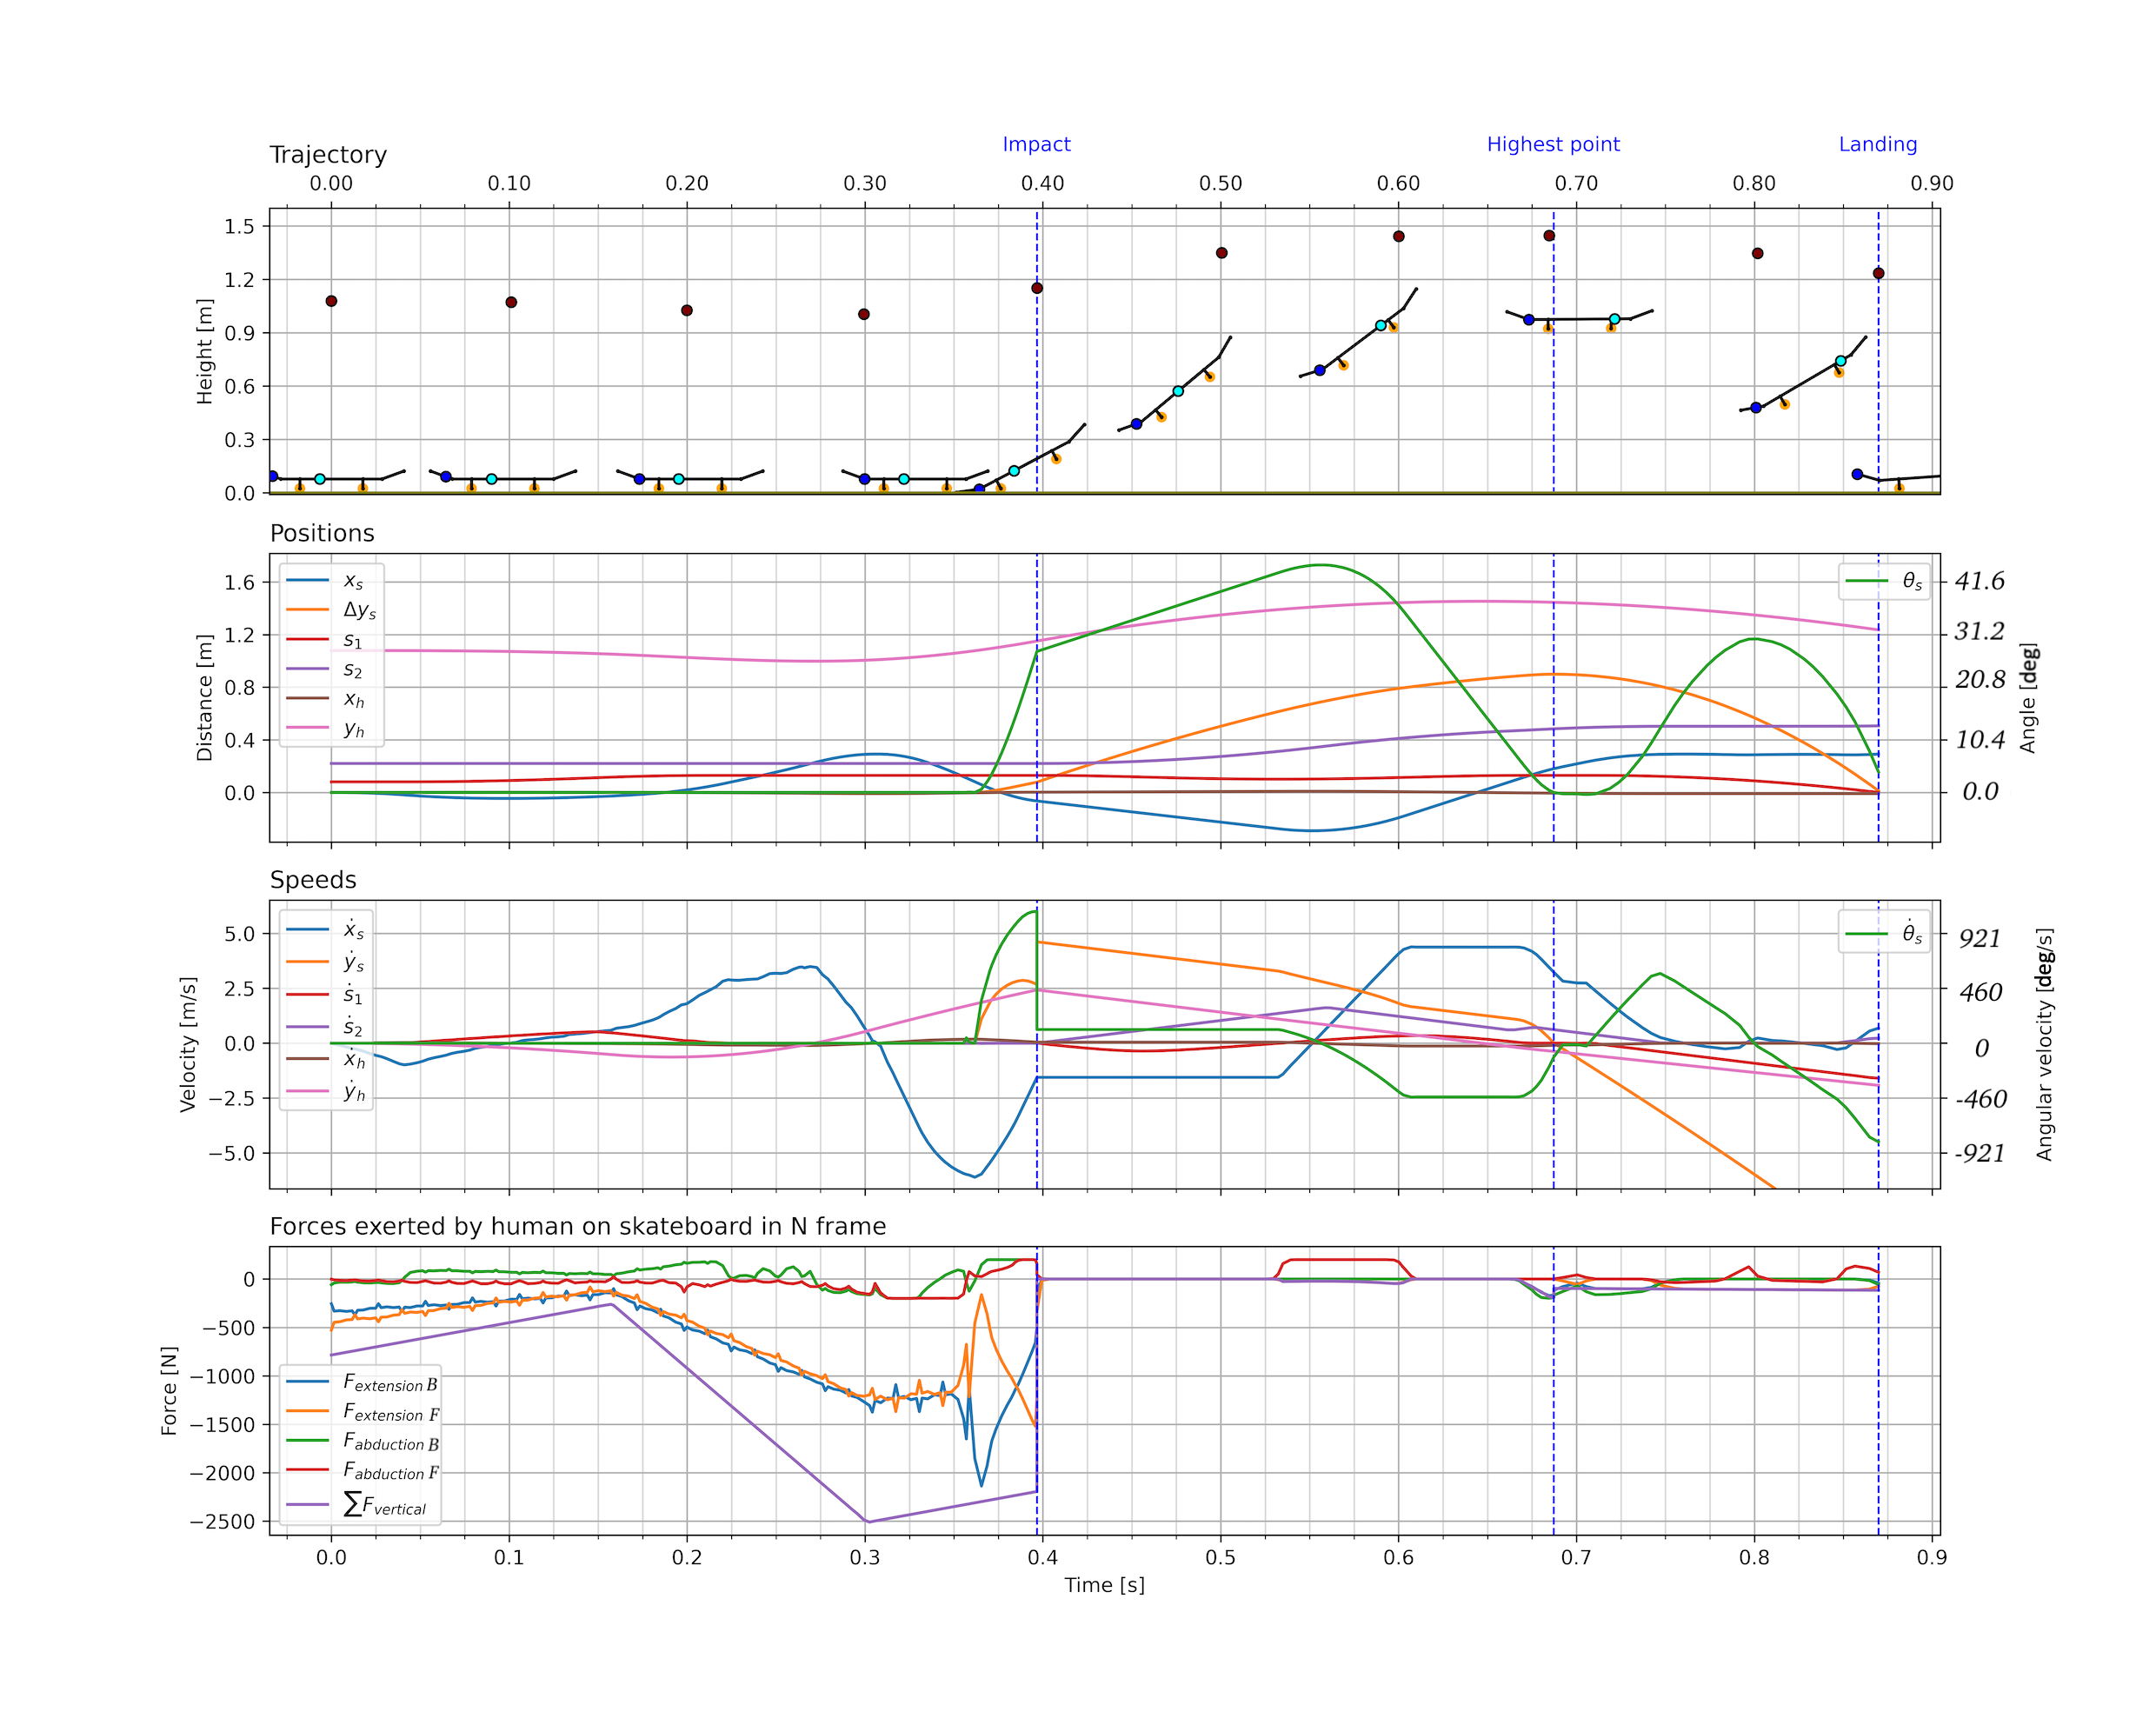
\includegraphics[trim={0cm 0cm 0cm 0cm},clip,width=\textwidth]{figure/Results/data_l_wbdpi600.png}    \vspace{-1cm}\caption[Trajectory, positions, speeds, and forces for wheelbase optimization]{Detailed trajectory of optimized wheelbase}\label{f_wheelbase}
    Corresponds to result 2. Wheelbase in figure \ref{f_singlepar}. 0.09[m] smaller wheelbase compared to base, 0.023[m] higher ollie. Three striking differences, the first is that the jumping force is now equally dependant on the back and front extension force (blue,orange,4), the second is that there is only one force peak between impact and highest point. The third striking part is that the skateboard rotates before landing (t=0.8).
\end{figure*}
\noindent The next optimization concerns the single parameter optimization shown in figure \ref{f_wheelbase}. The wheel base of the skateboard is optimized along with optimal control. Most of the phenomena seen in the base optimization are also visible for this optimization. The human lowers their weight, pushes the skateboard forward then pulls it backward. Angular velocity is lost during impact (-1193 [deg/s] and vertical speed is gained (green and orange lines speeds). After impact abduction force with the front leg is used to pull the skateboard up and level it out. The first difference is visible in the force plot. The sum of the vertical forces (purple line) does not stagger when unloading. A straight line up, down, and then up is achieved. Secondly, a higher angular velocity is achieved compared to the base. The back foot is once again in the pocket of the board, but now the front foot is at equal distance from the wheel having perfect balance. At this position both legs can exert equal force without rotating the board during eccentric braking ($t=0.15 - 0.3$). Then suddenly shortly before the impact, the front foot (orange line forces) pulls up and the back foot pushes down to create a maximal momentum about the back axis creating a steep sudden increase in angular velocity. The decreased wheelbase causes the impact angle to be lower and the angular velocity near zero just after impact (green lines positions and speeds). This leaves a period of rest such that the skateboard can gain height. While the front foot is in a sliding motion, the foot starts pushing down on the board at t=0.53.  This is almost enough to level the board out at the highest point. But the negative angular rotation caused by this push is caught with the back foot at the highest point making sure the board is leveled. 
The reason why this board can ollie higher is because it needs less force input during the upward motion to level the board out and is able to reach higher angular velocities due to reduced inertia. By decreasing the wheelbase, the inertia of the skateboard is decreased. With a decreased inertia, the dynamic response is faster resulting in higher angular velocity with the same amount of torque produced. Also less force is needed to level the skateboard during the upward motion because the same amount of force input will result in a larger angular deflection compared to the base skateboard. 

\begin{figure*}[t]
    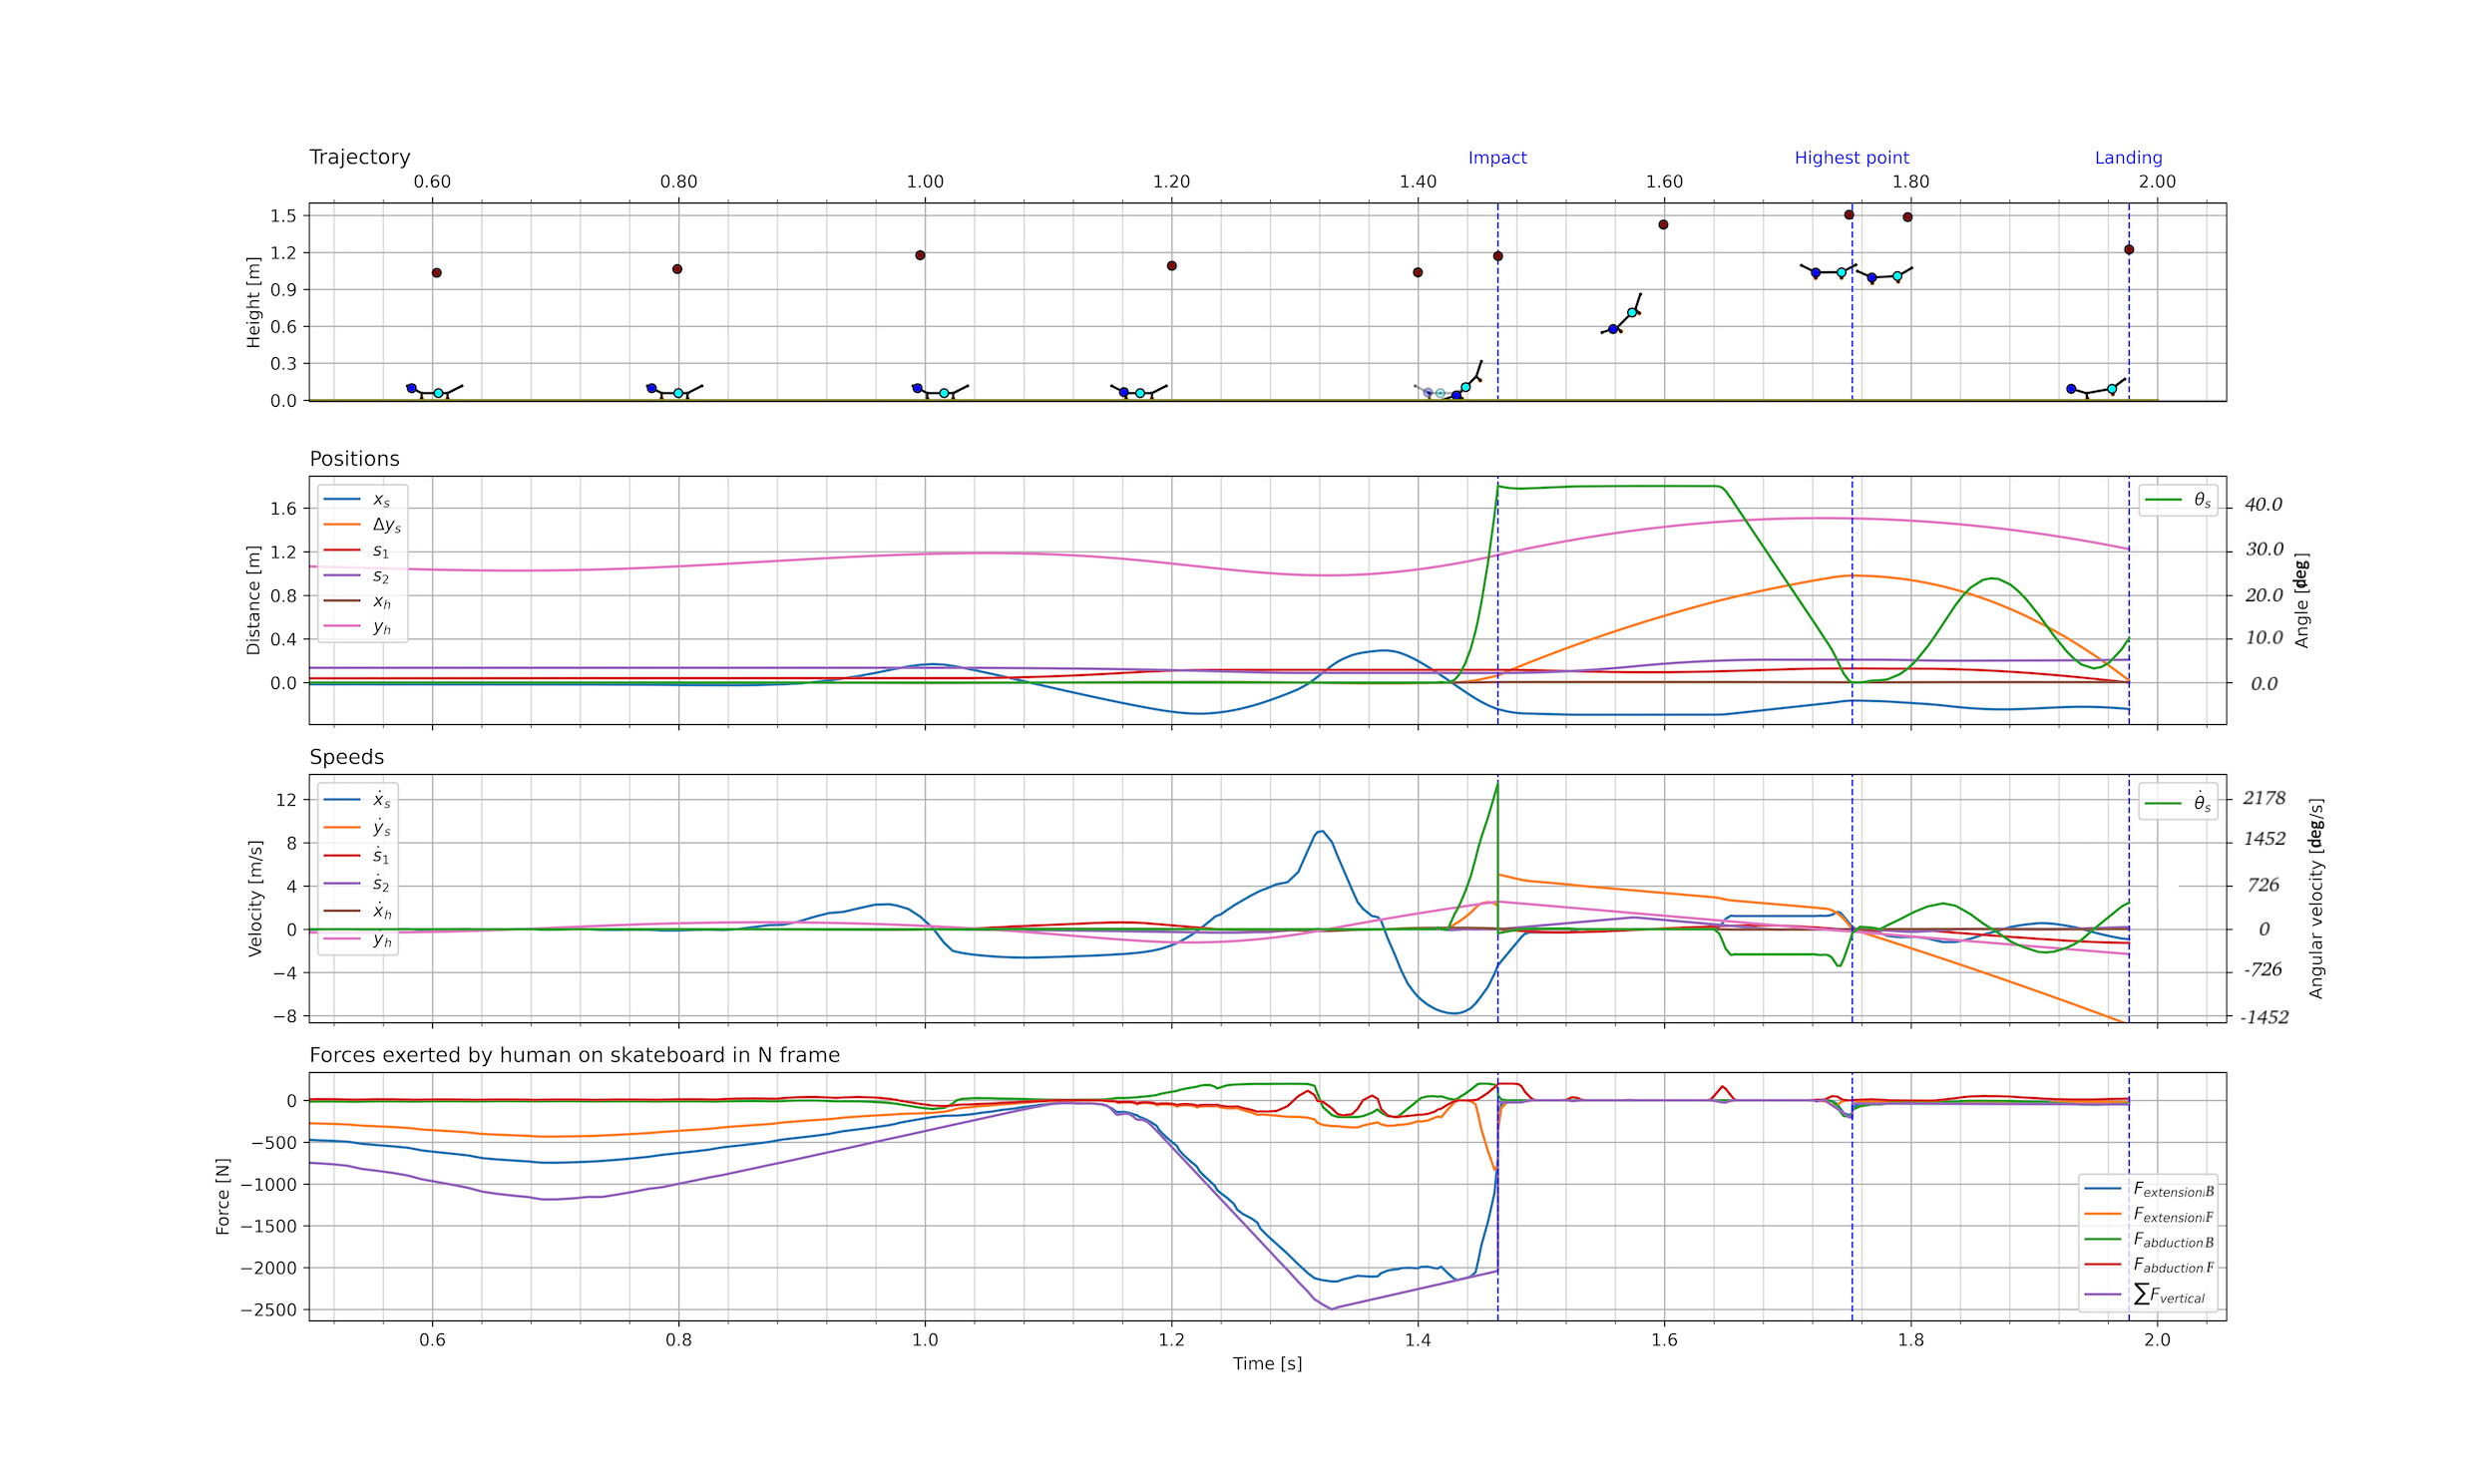
\includegraphics[trim={0cm 0cm 0cm 0cm},clip,width=\textwidth]{figure/Results/data_no_taildpi600.png}
    \caption[Trajectory, positions, speeds, and forces for `all except tail length' optimization]{Detailed trajectory of optimization of all parameters except the tail}\label{f_notail}
    Optimization `no $l_t$'. Corresponds to result 2. No $l_t$ in figure \ref{f_multipar}.
    
\end{figure*}
\begin{figure*}[t]
    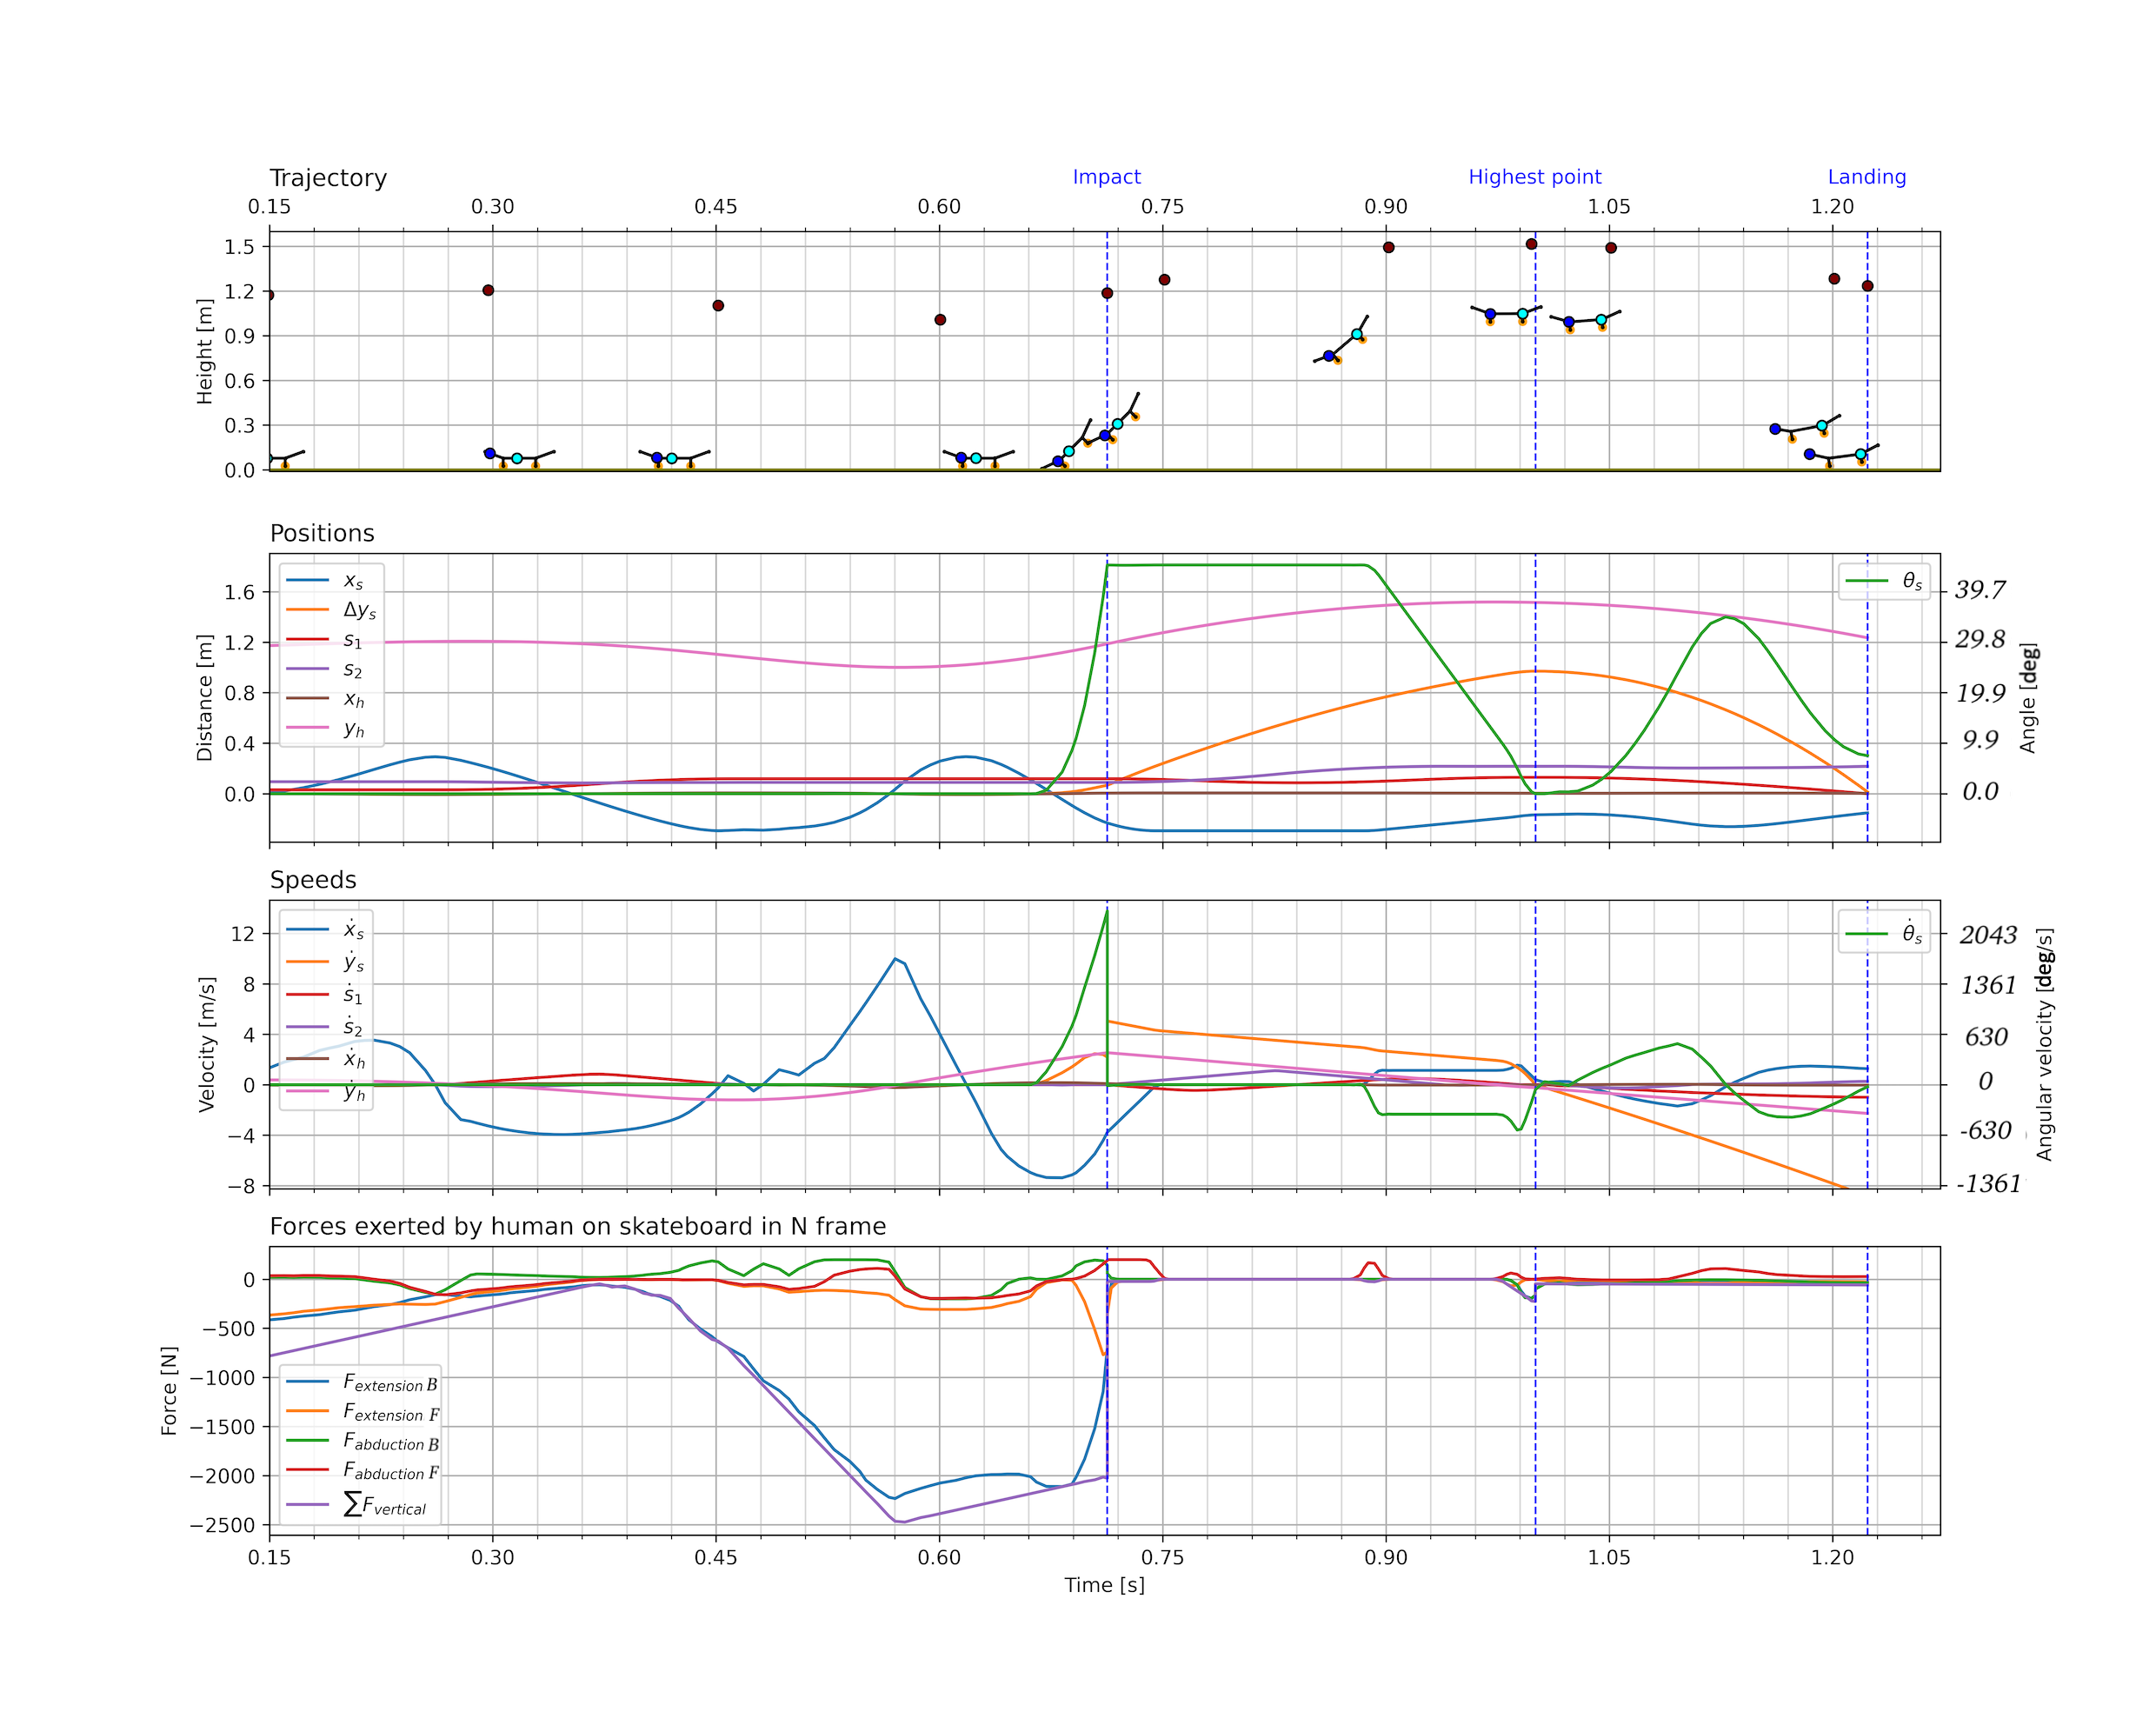
\includegraphics[trim={0cm 0cm 0cm 0cm},clip,width=\textwidth]{figure/Results/data_notrrwltdpi600.png}
    \vspace{-0.5cm}\caption[Trajectory, positions, speeds, and forces for `deck except tail length' optimization]{Detailed trajectory of optimized Wheelbase, tail inclination, and deck length}\label{f_notailnotruck}
    Corresponds to result 4. deck no $l_t$ in figure \ref{f_multipar}. The human first goes up and down before wanting to jump (pink,2). The time before impact is (long 1.46 [s]). The rotational speed at impact is 2178 [deg/s]. Between t=1.5 and t=1.8 there is almost zero force exerted, a small peak at t=1.7 is sufficient to level skateboard at highest point. At highest point the skateboard is behind the human.
\end{figure*}

\subsubsection{Multiple parameter optimizations}
\paragraph{All except tail}
\noindent In this optimization all variables but the tail are optimized shown in \ref{f_notail}. Compared to the base skateboard, this skateboard is able to ollie higher (0.106 [m]). Though a lot of similarities can be found between the two. The horizontal velocity is negative prior to impact, than after impact the board is dragged upward and forward. This skateboard is significantly easier to rotate due to the lower inertia and mass ($I_s = 0.02 [kg m^2]$ compared to $0.122 [kg m^2]$ for the base skateboard and $m_s = 1.459 [kg]$ compared to $2.377 [kg]$ for the base skateboard). Due to these lowered variables, with the same amount of force over time the angular velocity that is obtained is twice as high. (green line speeds). It is worth noting that the human jumps highest with this skateboard setup. 
With this setup the skateboarder is able to jump almost solely from its back foot (blue line forces) due to the fact that the foot is located almost exactly above the back wheel such that there is no or little momentum created about the back axis. 

\paragraph{Wheelbase, tail inclination, and deck length}
\noindent In this optimization the truck height and wheel radius are not optimized as shown in figure \ref{f_multipar}. The trajectory, positions and speeds of this skateboard are very similar to the prior optimization. The mass and inertia have increased due to the higher weight of the wheels compared to the previous optimization.

\section{Discussion}
\noindent The skateboard trajectories are all very similar to an actual ollie. Without any motion cues, the optimizer is able to replicate the ollie motion, with almost all phenomena seen in \ref{fig:ollie steps}. The optimizer shows that the human first jumps, then slams the skateboard to the ground, slides the front foot over the deck to drag it up and level it out and catches the skateboard with the back foot at the highest point. This is very close to reality. The human replicates the counter movement jump with a very similar force graph if figures \ref{f_notail} and \ref{fig:GRF} are compared. Also the impact energy is similar to the impulse found in figure \ref{fig:GRF}. The impulse from the \gls{grf} is roughly \SI{5}{\joule}, which is of the same order of magnitude as the found impact losses in figures \ref{f_nopar}, \ref{f_singlepar}, and \ref{f_multipar}.
A single mass point with two free floating feet controlled by forces and feet location with kinematic constraints are able to simulate the motion and output of a human jumper. 
Nine out of eleven optimal skateboard geometries found higher ollies compared to the popsicle stick skateboard. None of these solutions is proven a global optimum, but the improvement to the base skateboard is something that performs better. Skateboard builders should try to implement found geometries and test empirically if they will improve ollie height. These geometries could be a tool to alter existing skateboards and let athletes jump higher. The kinetic and kinematic constraints are of a specific person. The geometries might be dependent on the human capabilities. Empirical testing is necessary to prove that this finding is true in a real life ollie. I successfully solved the ollie optimization problem with a geometry optimization. Compared to others Shield et al. \cite{shield_contact-implicit_2022} who solved an optimization problem for the ollie, my optimization was faster (3 min vs. 43 min), included an geometry optimization, and had a more difficult objective function. The Shield optimization was was set at a fixed ollie height and needed motion tracking to solve optimally. My optimization had a null seed initial guess, with an objective function that maximized ollie height. Such objective functions are generally hard to solve, for example in \cite{nitschke_efficient_2020} first tracking data needs to be implemented to solve a more difficult objective. Step by step less data can be used to solve for an more difficult objective. In the case of this paper, the solution is found without any tracking data and a difficult objective function. 
\subsection{Findings}
\noindent\textbf{Lower inertia and skateboard mass is beneficial for ollie height.} In all parameter optimizations that improved ollie height compared to the base, a reduction in mass and inertia is found.

\noindent\textbf{Popsicle stick skateboard is close to optimum and slight changes due to preference will not influence the ollie height too much.} The increase in ollie height was minimal (0.05-0.023 [m]). If skateboarding will keep the popsicle stick skateboard as standard due to the fact that other tricks need to be performed other than the ollie, not much can be changed to the skateboard to optimize it. The wheelbase effects the ollie height the most of all single parameter optimizations, which could be a promising outcome since it does not influence the board shape which is crucial for other tricks. 

\noindent\textbf{Extremely fast optimal solution is found and easy convergence.} The ollie optimization by Shield et al. \cite{shield_contact-implicit_2022} was without a parameter optimization of the skateboard. This optimization took about 43 minutes to solve, and accurate initial guesses were needed for feasible results. The full code presented by me took under 3 minutes to solve. This includes derivation of the Equations of Motion and all constraints, the time to transcribe the problem and to solve in IPOPT. This was all done without initial guesses and solved optimally.

\noindent\textbf{Optimal back foot position is influenced by the leg characteristics of the performer.} The controller preferred high force outputs over high foot velocities. This is why the back foot always sits in the back pocket during the optimization.
%For example imagine a simple lever system with a fixed force magnitude perpendicular to the lever with distance x from the rotation point. The higher x, the more torque can be generated, but the greater the distance ($s$) the force will travel. In other words $P = F \delta s = F v $. With a fixed power there has to be a trade of between force and velocity. In this case velocity of the back foot is minimized by setting the back foot in the pocket. According to a jumping theory by Morin an Samozino \cite{morin_biomechanics_2018}, jumping output is bound by a force velocity curve, where maximum force can be exerted at zero speed and maximum velocity at zero force. Athletes have different force velocity profiles where one prefers high force output over high velocity and vice versa. The controller preferred the force profile by minimizing the back foot velocity. This finding leads to the conclusion that athletes with different leg profiles should place their feet differently during the ollie. Where a force-profile should set the back foot in the pocket and a velocity-profile on the tip of the skateboard. See figure \ref{FVcurve} for force and velocity oriented human leg output.

% \begin{figure}
%     \centering
%     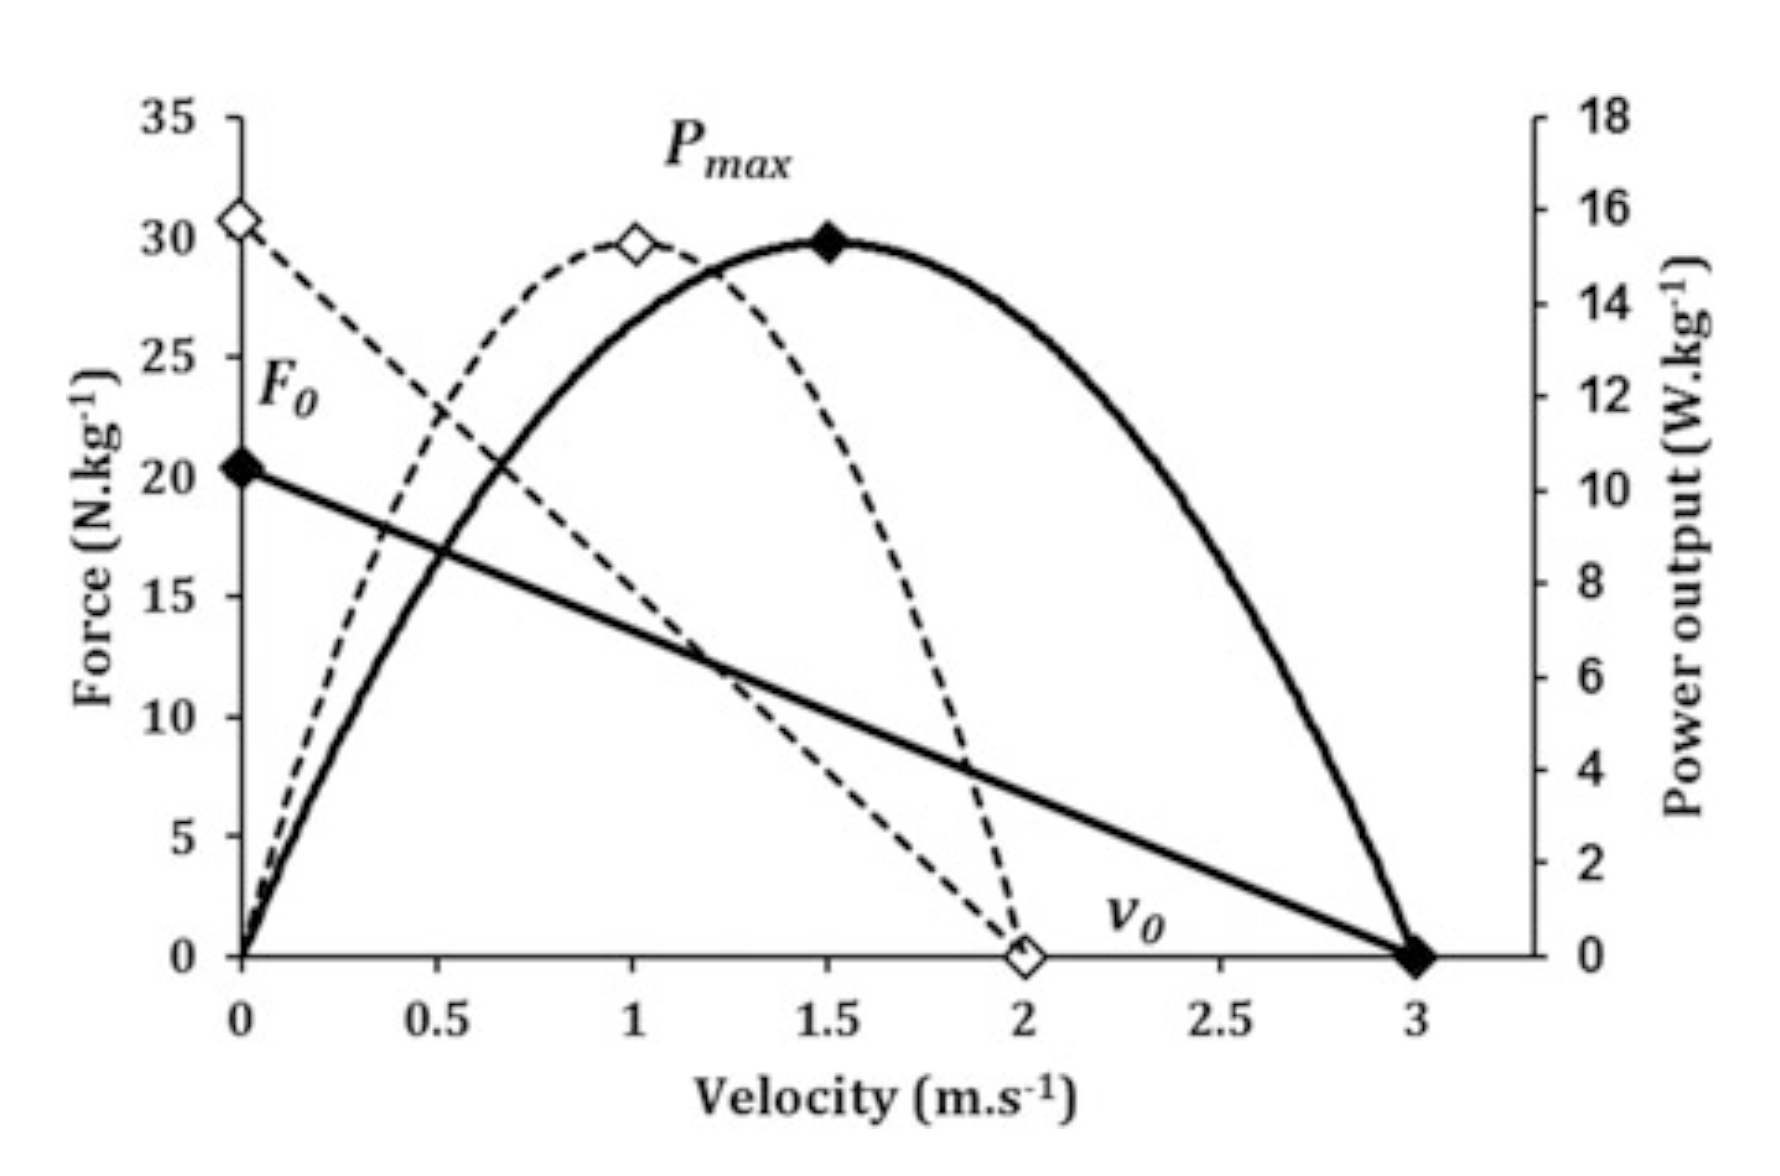
\includegraphics[width = 0.4\textwidth]{figure/Schermafbeelding 2022-11-21 om 16.08.08.png}
%     \caption[F-v curve]{Theory on human leg output during jumping. When increasing the load, the maximal force and velocity stay on the line. The dotted line shows a more force oriented human, whereas the other shows a more velocity preferred human jumper. Both have the same maximal power output}
%     \label{FVcurve}
% \end{figure}

%\noindent\textbf{Highly adoptable model.} The presented model can be adjusted to the kinetic and kinematic bounds with little effort. The possibility to optimize a skateboard for a specific athlete is not hard to implement but the kinetic data should be present. Also preference bounds such as width are easily implemented.

%\noindent\textbf{Inertia and mass model inertia and mass model for a skateboard is presented that can estimate the dynamic board behaviour in 2D}. The model should be verified with multiple skateboard geometries.

\noindent\textbf{Well represented kinetics.} All results show high similarities between the force profiles of the counter movement jump seen in figure \ref{f_cmj}. The sum of the human kinetics are well bound and show constant results. Even though it is a highly simplified model, the output of the forces is very similar to the output of a CMJ. The point mass model is insightful for the dynamics and is able to show valid results. \\

\noindent\textbf{A fundamentally different simplified contact implicit optimization is made.} The relaxed formulation by Patel et al. \cite{patel_contact-implicit_2019} has been simplified by restating the contact definition. Static and dynamic friction is achieved with the ability to have contact implicit events.

\subsection{Limitations and Future research}
\noindent\textbf{Tail length optimization leads to local maxima.} As seen in the results the tail length optimizations showed lower ollie height compared to the same optimizations with restricted tail length. This is per definition a local maximum because the solution space of the optimization with tail length optimized should contain the restricted tail length optimization solution. In real life a longer tail length would cause a higher energy dissipation due to more bending during impact. A plausible cause for these local maxima is that impact loss is of too little effect. When a human jumps, the order of magnitude of the amount of energy necessary to go up is in the order of $10^3$. The dissipation of energy during impact is in the order of $10^{-1}$. This means that the impact loss could be of so little effect to increasing ollie height that the solution space has become very flat. You can see that the model does capture the increase impact loss. When the tail length is optimized and the large tail length solution is found, there is an increase of 227\% compared to the base optimization. Maybe if the impact loss would be penalized more, optimal tail lengths will be found.
 
% Range of motion, balance, spacial skeletal constraints
\noindent\textbf{Lack of complexity in the kinematic constraints of the human controller.} Due to the simplification of a human as a mass point with two feet, kinematic constraints are highly simplified. In real life a penny board is difficult to ollie due to the fact that the operating area is really small. The feet would have to operate precise and powerful movements while balancing on a small surface. While the controller can easily do this, it does not represent reality completely. Also inertia of the human is neglected due to the simplification.

\noindent\textbf{Front wheel normal force.} In future research it is advised to implement a normal force acting on the front wheel during the preparation phase. The front foot had to counteract the rotation created by the back foot. In real life the front foot could have been on any location without causing a counter clockwise rotation due to the compensation of the normal force. Difficulties will be to find a phase switch cue for the optimizer. It might be possible to set a fixed time for the first phase to solve this.

\noindent\textbf{Possible that current solutions are not global optima, more optimal board shapes can be found.} The presented solution space is very large due to many possibilities in variables. In future research, many more geometries can be found which could help the skateboard community to understand the dynamics of the ollie. 

\noindent\textbf{Extra constraints should be implemented to the legs individually.} Now single leg behaviour can sometimes exceed human limitations. Due to a lack of data on single leg jump for one specific athlete together with the CMJ information the single leg behaviour is not yet fully bound by human limitations.

\section{Conclusion}
\noindent A model is made to optimize the skateboard for ollie height with a human controller. Optimal board shapes have been found that show higher ollie performance than the current popsicle stick skateboard. The research question 
\begin{quote}
\textit{What are the optimal geometric and inertial parameters of a skateboard for an Olympic athlete to reach maximal ollie height? 
}\end{quote}
has not been answered fully but a closer approximation is given towards the optimal shape for maximal ollie height and more insight is gained in the dynamics of the ollie. Though, the process of creating a model to optimize the skateboard ollie has been an exploration of the endless variables in the movements of both athlete and board. One conclusion is the fact that the created model turned out to be surprisingly close to the real world. The model is a user friendly and quick tool to find optimal board shapes dependent on the kinetics of a human performer. The kinetics can easily be implemented by any researcher or any skateboarder that is in the possession of a force plate. Making this model a very agile and useful tool for skaters, skateboard manufacturers and future researchers. Although the research question is not fully answered, the outcome of all the different optimizations gives a lot of insight in the dynamics of the ollie. This insight could be an inspiration to other researchers, skateboarders and board builders to expand and develop the academic comprehension of the dynamics of skateboarding. 

\bibliographystyle{asmems4}
\bibliography{references}

\section{Appendix: Equation of Motion Derivation}
% Differentiating $\mathbf{x}$ once and taking the Jacobian with respect to the
% velocities gives transformation matrix $\mathbf{T}$:
% %
% \begin{equation}
%     J_{\dot{\mathbf{x}}}(\mathbf{q}) = \textbf{T} = \left[\begin{array}{c c}
% 1 & -\frac{l_{w b} \sin \left(\theta_s\right)}{2}+\left(d_{c o m}-h_{t r}\right) \cos \left(\theta_s\right) \\
% 0 & \frac{l_{w b} \cos \left(\theta_s\right)}{2}+\left(d_{c o m}-h_{t r}\right) \sin \left(\theta_s\right) \\
% 0 & 1
% \end{array}\right]
% \end{equation}

% Convective terms $\mathbf{g_k}$ are found by taking the Jacobian of $\mathbf{\dot  x}$ with respect to $\mathbf{q}$ and multiplying it by $\mathbf{\dot  q}$ (e.g. $J_{\mathbf{\dot  x}}(\mathbf{q})\cdot \mathbf{\dot  q}$):

% \begin{equation}
% \mathbf{g_k} = 
% \left[\begin{array}{c}
% \dot \theta_s^2\left(-\frac{l_{w b} \cos \left(\theta_s\right)}{2}-\left(d_{c o m}-h_{t r}\right) \sin \left(\theta_s\right)\right) \\
% \dot \theta_s^2\left(-\frac{l_{w b} \sin \left(\theta_s\right)}{2}+\left(d_{c o m}-h_{t r}\right) \cos \left(\theta_s\right)\right) \\
% 0
% \end{array}\right]
% \end{equation}
\pagestyle{plain}
%\onecolumn
\section*{Appendix A}

\subsection*{Mesh example}
 By default each phase is subdivided into 10 mesh sections. Each mesh sections has 4 collocation points where the last of mesh section $n$ overlaps with the first collocation point of mesh section n+1 and so on. Thus each non beginning section has two overlapping points, this is the definition of the LGL method. This means by default each phase uses 31 collocation points. Mesh refinement is done when the mesh error did not reach the mesh tolerance. If the mesh section did not meet the tolerance, estimated $k$ extra collocation points are added to the mesh section. This means that the polynomial in the mesh section increased to the order $4+k$. This process will go on until the mesh tolerance is met or $k$ is estimated at a number that will exceed a 10th order polynomial. In this case the mesh section will be split up in new smaller sections. The sections will be split into parts that will match the expectation to 4 collocation points. For example, when the estimation of a 'correct' integration is estimated at 13 collocation points, the section will be split into four equally sized sections. When the estimation is to need 17 collocation points, 5 sections will be created. This method should be numerically efficient, since only the sections that show high nonlinearity and need a finer mesh will be integrated more thoroughly. If the tolerance is already met with a lower order integration, there will be no refinement\cite{rao_survey_2010,brockie_predictive_nodate,fasano_space_2016}. 

\section*{Mass, centre of mass and inertia model}


\section*{Inertia measurement}
To verify the inertial values obtained in the parameterized model of the skateboard, the inertia of two arbitrary skateboards are measured. 
\subsection*{Theory}
The skateboards inertia is measured by approximating the board as a compound pendulum. The inertia in a compound pendulum is directly related to the period of the swing of the pendulum. The torque produced by gravity is:
$$
\alpha I_o=-L m g \theta
$$
Using that the angular acceleration $(\alpha)$ can also be written as $\frac{d^2 \theta}{d t^2}$, we can re-write the angular acceleration as follows:
$$
\frac{d^2 \theta}{d t^2}=-\left(\frac{m g L}{I_o}\right) \theta
$$
This is a second order differential equation, for which we can use the standard solution for $\frac{d^2 \theta}{d t^2}=-b \theta$, which gives $\theta(t)=\cos (\omega t+\phi)$ with $\omega^2=b$. This results in an expression for the angular speed $(\omega)$ :
$$
\omega=\sqrt{\frac{m g L}{I_o}}
$$
Now that we can see the correlation between the period and the inertia of the compound pendulum, we can find the inertia about the COM of the skateboard by applying the parallel axis theorem:
\begin{equation}
    I_c = I_o + m L^2
\end{equation}
\subsection*{Method}
The skateboard was hung by ropes as seen in figure \ref{f_testsetup}. With a Silicon Sensing CRS43 gyroscope the rotational speed was measured. The skateboard was swung for 15 seconds released from 5, 10 or 15 degrees. The measured data was fit to a damped oscillation with a non linear least square method from SciPy. From the measured period the inertia values have been calculated giving the following fitted data shown in figure \ref{f_dampedoscillation}.
\begin{figure}
    \centering
    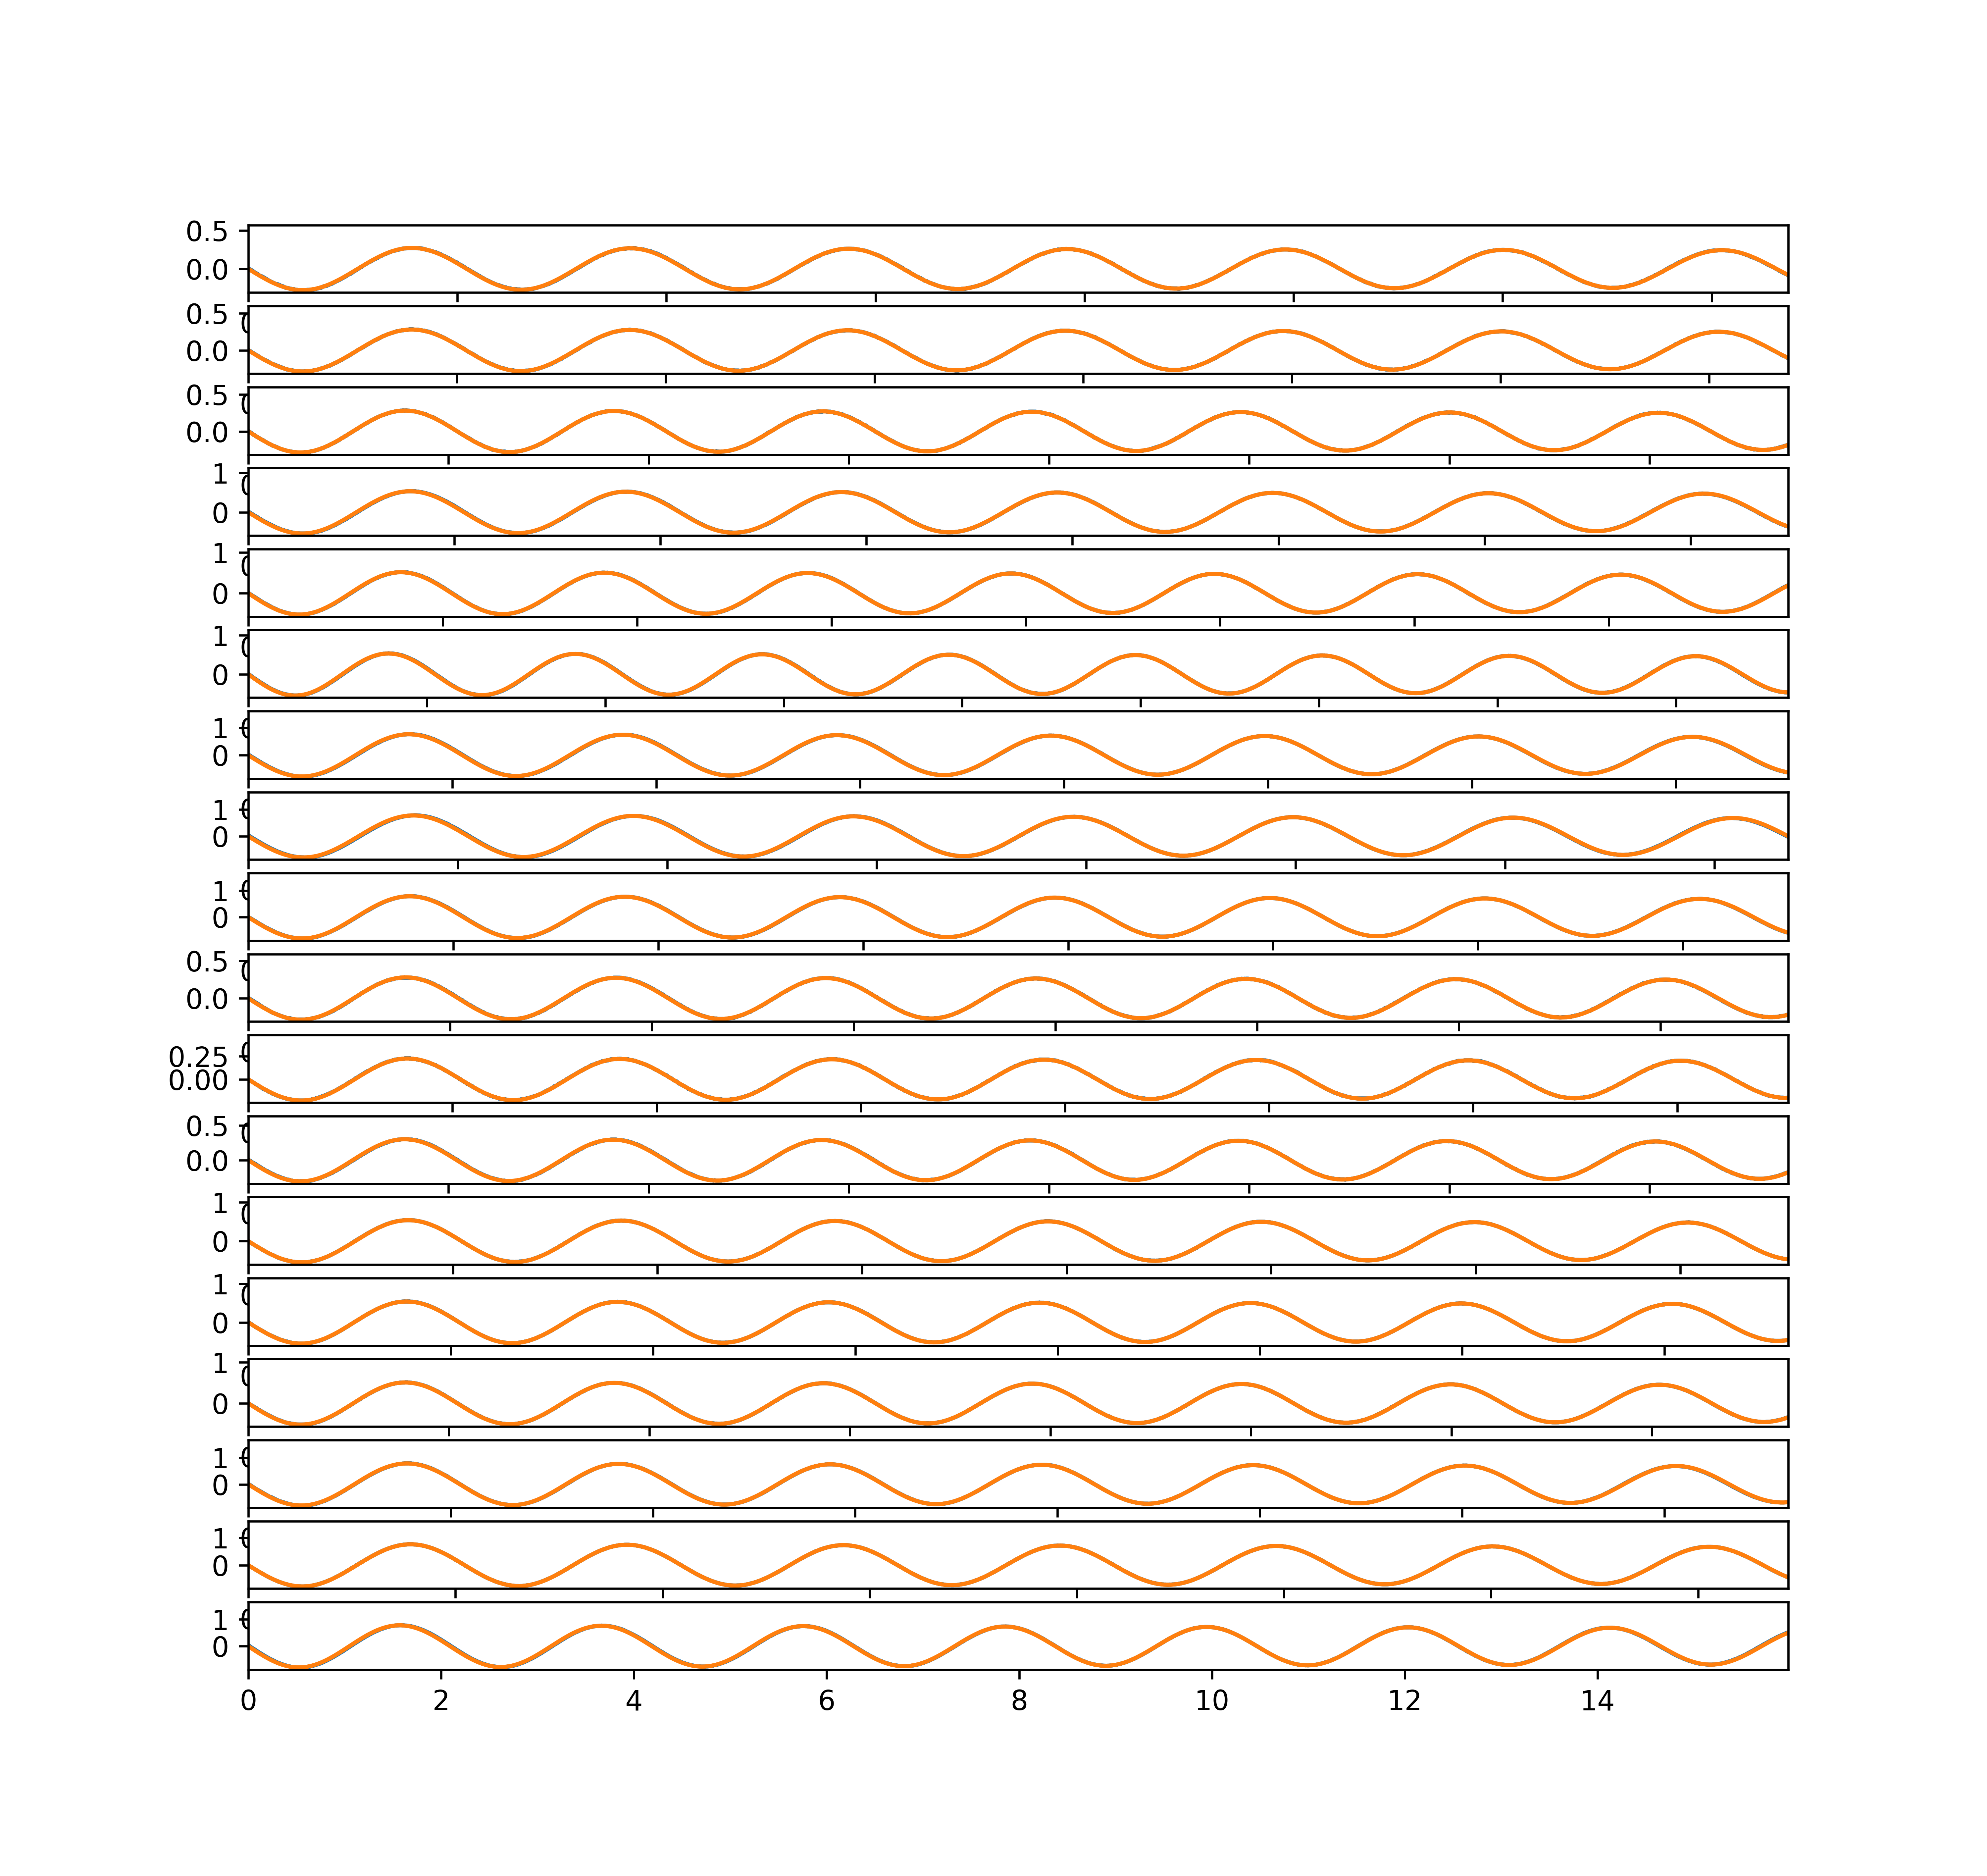
\includegraphics[width = 0.5\textwidth]{figure/damped_oscilation_fitdpi600.png}
    \caption{Fit of skateboard as compound pendulum}
    \label{f_dampedoscillation}
\end{figure}
The inertia results are given in figure \ref{f_inertianopower}
\begin{figure}
    \centering
    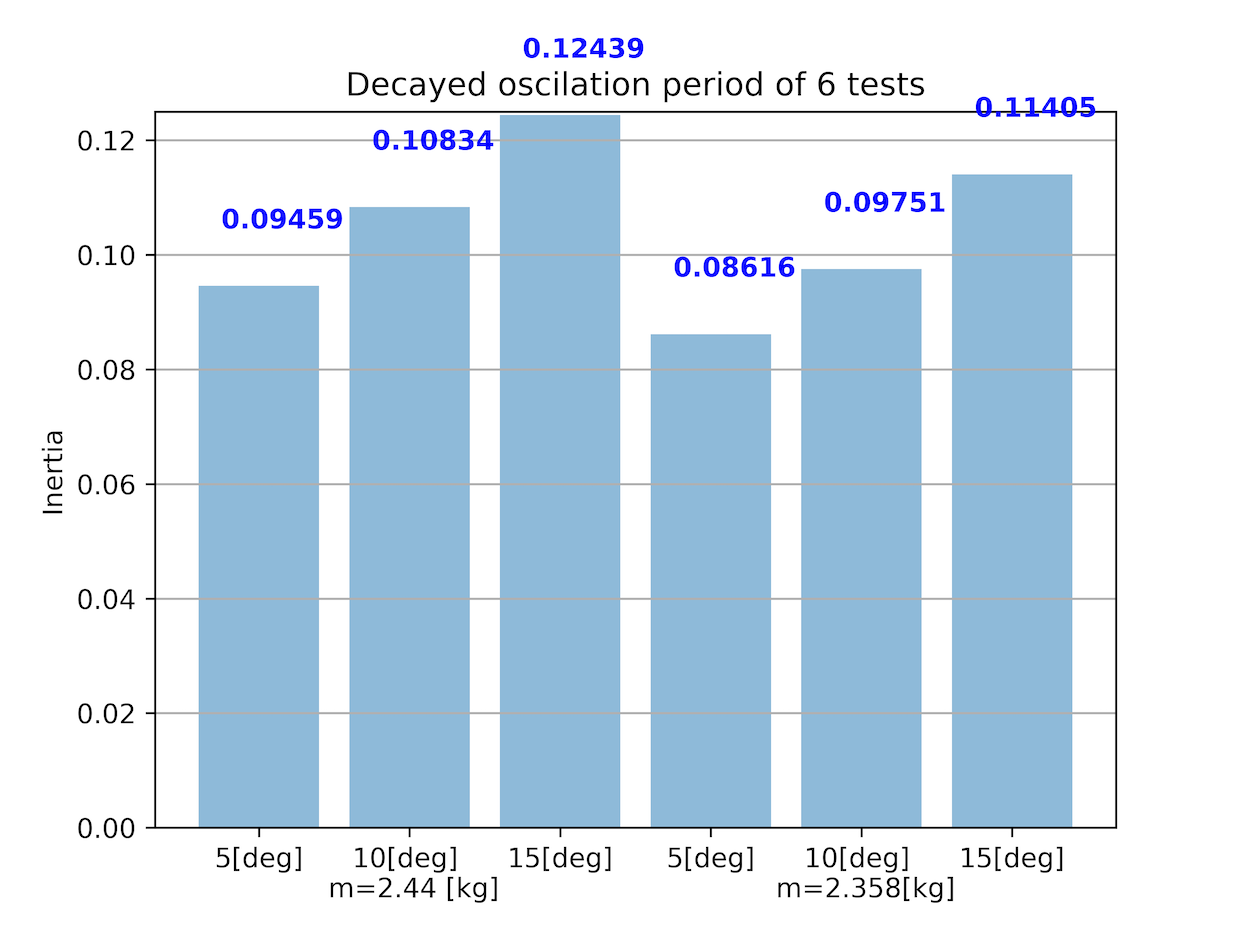
\includegraphics[width = 0.4\textwidth]{figure/Inertia_result_nopowerexpansiondpi600.png}
    \caption{Inertia results}
    \label{f_inertianopower}
\end{figure}
When it was clear that the inertia increased with an increase in starting angle, a power expansion is applied that accounts for small angle errors given by:
\begin{equation}
\begin{array}{r}
\omega_{exact} =  \approx T_0\left(1+\frac{1}{16} \theta^2+\frac{11}{3072} \theta^4+\frac{173}{737280} \theta^6\right. \\
\left.+\frac{22931}{1321205760} \theta^8+\ldots\right) .
\end{array}
\end{equation}
Which is used until the with precision $O^6$ results in the inertia data presented in figure \ref{f_powerexp}

\begin{figure}
    \centering
    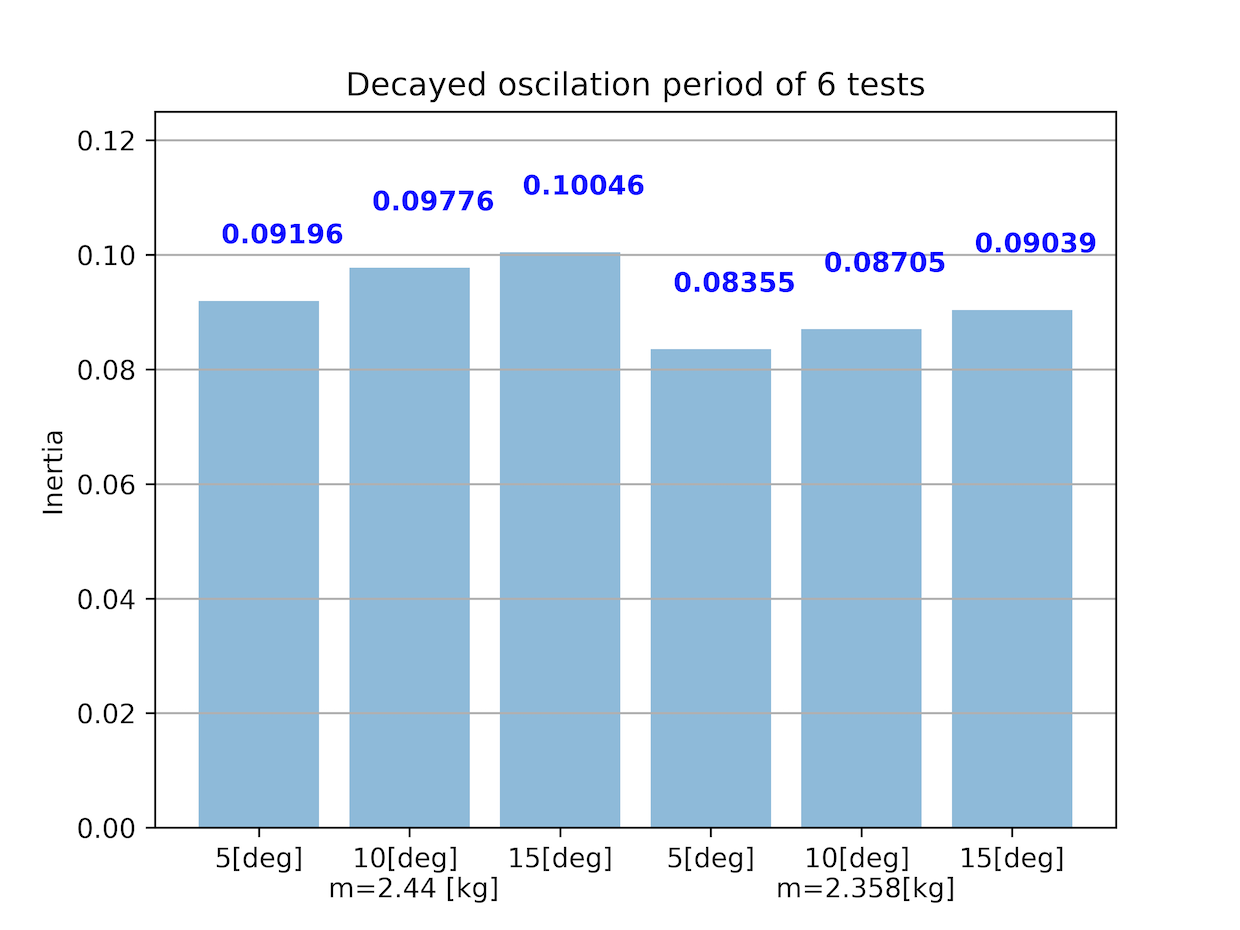
\includegraphics[width = 0.6\textwidth]{figure/Inertia_result_powerexpansiondpi600.png}
    \caption{Inertia result with power expansion}
    \label{f_powerexp}
\end{figure}

The calculated inertia value for skateboard with $m=2.44$ with the parameterized model is: 0.1219 [$kg\ m^2$]. The results show 0.09196 - 0.10046 [$kg\ m^2$]. The skateboards' inertia calculated with the parameterized model  with $m= 2.358$ is 0.1151 [$kg\ m^2$], while the results show 0.08355 - 0.09039 [$kg\ m^2$]. Both skateboards the model slightly overestimates the inertia.   The reduction in real life between the skateboards is 0.909\%, 0.890\%, 0.900\% between the different take off angles and different boards. In the parameterized model reduces inertia by 0.94 \%. This is of similar magnitude but needs more data to make it more exact. As a scaling approximation the parameter model is good enough.

\begin{figure}
    \centering
    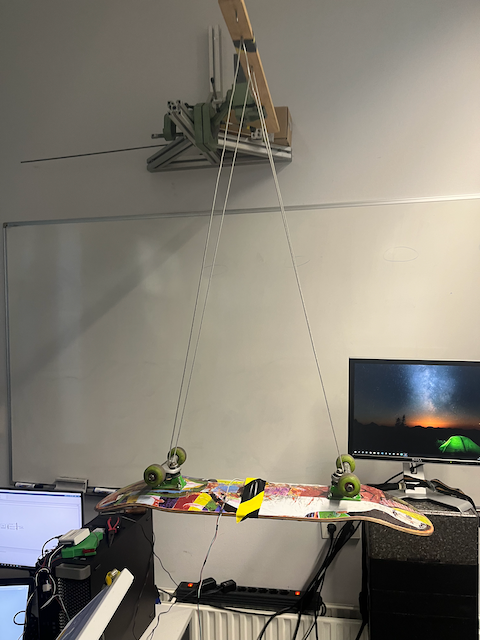
\includegraphics[width = 0.4 \textwidth]{figure/Testsetup.png}
    \caption{Test setup for inertia testing}
    \label{f_testsetup}
\end{figure}

\newpage
.
\newpage
\section*{Mass, centre of mass and inertia model}
\begin{verbatim}
    def Mass_model(width_deck, mass_bearing, mass_truck, height_truck, 
               height_truck0, width_wheel, n_ply, length_flat, length_tail, 
               radius_wheel, rho_pu, rho_maple, rho_steel, m_glue, 
               diameter_axle, d_veneer):

    mass_wheel = rho_pu * sm.pi * width_wheel * \
        ((2*radius_wheel)**2-diameter_axle**2) / 4  # V=pi*h*(D^2-d^2)/4

    mass_axle = sm.pi * (diameter_axle/2)**2 * width_deck * \
        rho_steel  # weight of axle, volume * steel * density

    #    _   _   ___________   _   _
    #  /  | | | |           | | | |  \
    # | 1 | |2| |     3     | |4| | 5 | 6=t1 7=w1 8=t2 9=w2
    #  \ _| |_| |___________| |_| |_ /

    #     1\                  /5
    #      2\_______3________/4
    #        6 \/         \/ 7
    #        8 O 9      10 O 11
    
    # Area of wooden components
    A1 = (1/2) * (1/4) * sm.pi * width_deck**2  # 1/4 pi d^2
    A2 = (length_tail - (width_deck/2)) * width_deck         # l * b
    A3 = length_flat * width_deck           # l * b
    A4 = A2
    A5 = A1
    
    thickness = n_ply*d_veneer
    dV = thickness*rho_maple+(m_glue/2*(n_ply-2))

    m1 = A1 * dV
    m2 = A2 * dV
    m3 = A3 * dV
    m4 = m2
    m5 = m1
    m6 = (mass_truck - mass_axle) * height_truck/height_truck0
    m7 = m6
    m8 = mass_axle
    m9 = 2*mass_wheel
    m10 = m8
    m11 = m9

    mass = [m1, m2, m3, m4, m5, m6, m7, m8, m9, m10, m11]
    return mass

def COM(mass, com_points, reference_point):
    # Function gets vector position from reference_point
    # Then assigns COM location to point COM
    # Returns position vector of COM points relative to COM
    r_m = []
    for i, x in enumerate(com_points):
        r_m.append(x.pos_from(reference_point)*mass[i])
    COM_skateboard = me.Point('COM_skateboard')
    COM_skateboard.set_pos(reference_point, (sum(r_m)/sum(mass)))
    return COM_skateboard
\end{verbatim}
\newpage
\begin{verbatim}
    
def Inertia_model(mass, com_points, com, majordim, shape):
    # Major dim:
    #   - (semi)cylinder;  diameter
    #   - cuboid: [l,h]
    #   - Triangle: [Base, Height]

    I_com = []
    I_steiner = []

    for i in range(len(mass)):
        if shape[i] == 'semicircle':
            I_com.append(((1/4)-(16/(9*sm.pi**2)))*mass[i]*(majordim[i]/2)**2)

        if shape[i] == 'cuboid':
            I_com.append((mass[i]/12) * (majordim[i]
                         [0]**2 + majordim[i][1]**2))

        if shape[i] == 'triangle':
            s = sm.sqrt((majordim[i][0]/2)**2+majordim[i][1]**2)
            beta = 2*sm.asin((majordim[i][0]/2)/s)
            I_com.append((mass[i]/2)*s**2*(1-(2/3)*sm.sin(beta)))

        if shape[i] == 'cylinder':
            I_com.append((1/2)*mass[i]*(majordim[i]/2)**2)
        #Trigsimp was sometimes necesarry due to a theta still being in there
        I_steiner.append(sm.trigsimp(mass[i]*d2s(sm.sqrt(com_points[i].\
        pos_from(com).dot(A.x)**2+com_points[i].pos_from(com).dot(A.y)**2)**2)))
    I_tot = sum(I_com)+sum(I_steiner)
    return I_tot, I_com, I_steiner
\end{verbatim}

%\section*{Appendix B: Figures and tables}
\begin{table*}[h]
\begin{center}
\caption[Numerical bounds of state variables]{\centering Numerical bounds to state variables in the order of initial - absolute - final bounds. Final bound of $p^{(n)}$ equals initial bound of $p^{(n+1)}$. $v_{bound} = [-50,50]$} 
\begin{tabular}{r l l l l l l l l}\label{t_constraints}
& & \\ % put some space after the caption
\hline
ID         & Variable   & $p_0^{(1)}$ & $p^{(1)}_{bounds}$& $p_F^{(1)} = p_0^{2}$ & $p^{(2)}_{bounds}$ &$p_F^{(2)} = p_0^{(3)}$& $p^{(3)}_{bounds}$ &$p_F^{(3)}$  \\
\hline
\rownumber & $x_w$      & [-1, 0]     & [-2,1]            & [-2,1]               & -                  & -                   &  -                  & -\\
\rownumber & $x_s$      & -           & -                 &[-1,1]                & [-1,1]             & [-1, 1]             &  [-1,1]             & [-1,1]   \\
\rownumber & $y_s$      & -           & -                 &[0, 2]                & [0,5]              & [0, 5]              &  [0,5]              & [0,1] \\
\rownumber & $\theta_s$ & 0           & [0,$\pi$/2]       &[0, $\pi$/2 ]         & [-$\pi$/2 ,$\pi$/4]& 0                   & [$-\pi$/2, $\pi$/4] & [0, $\pi$/6]\\
\rownumber & $s_1$      & [0,1]       & [0,1]             &[0,1]                 & [0,1]              & [0,1]               & [0,1]              & [0,1]\\
\rownumber & $s_2 $     & [0,1]       & [0,1]             &[0,1]                 & [0,1]              & [0,1]               & [0,1]              & [0,1]\\
\rownumber & $x_h $     & 0           & [-1,1]            &[-1,1]                & [-1,1]             & [-1,1]              & [-1,1]             & [-1,1]\\
\rownumber & $y_h $     & [0,2]       & [0,5]             &[0,5]                 & [0,5]              & [0,5]               & [0,5]              & [0,5]\\
\rownumber & $\dot x_w$ & -           & $v_{bound}$       & $v_{bound}$          & -                  & -                   &  -                 &\\
\rownumber & $\dot x_s$ & 0           & $v_{bound}$       & $v_{bound}$          &$v_{bound}$         &$v_{bound}$          & $v_{bound}$        & $v_{bound}$  \\
\rownumber & $\dot y_s$ & 0           & $v_{bound}$       & $v_{bound}$          &$v_{bound}$         & 0                   &$v_{bound}$        & $v_{bound}$\\
\rownumber & $\dot \theta_s$ & 0      & $v_{bound}$       & $v_{bound}$          &$v_{bound}$         & $v_{bound}$         &$v_{bound}$        & $v_{bound}$ \\
\rownumber & $\dot s_1$ & 0           & $v_{bound}$       & $v_{bound}$          &$v_{bound}$         & $v_{bound}$         &$v_{bound}$        & $v_{bound}$ \\
\rownumber & $\dot s_2 $& 0           & $v_{bound}$       & $v_{bound}$          &$v_{bound}$         & $v_{bound}$         &$v_{bound}$        & $v_{bound}$ \\
\rownumber & $\dot x_h $& 0           & $v_{bound}$       & $v_{bound}$          &$v_{bound}$         & $v_{bound}$         &$v_{bound}$        & $v_{bound}$ \\
\rownumber & $\dot y_h $& 0           & $v_{bound}$       & $v_{bound}$          &$v_{bound}$         & $v_{bound}$         &$v_{bound}$        & $v_{bound}$ \\

\hline
\end{tabular}
\end{center}
\end{table*}
\section*{Results of optimal board shapes}
Detailed trajectories, states and control of all optimizations shown in figures \ref{f_nopar}, \ref{f_singlepar}, and \ref{f_multipar}
\begin{figure*}[b]
    \subfloat[Long board]{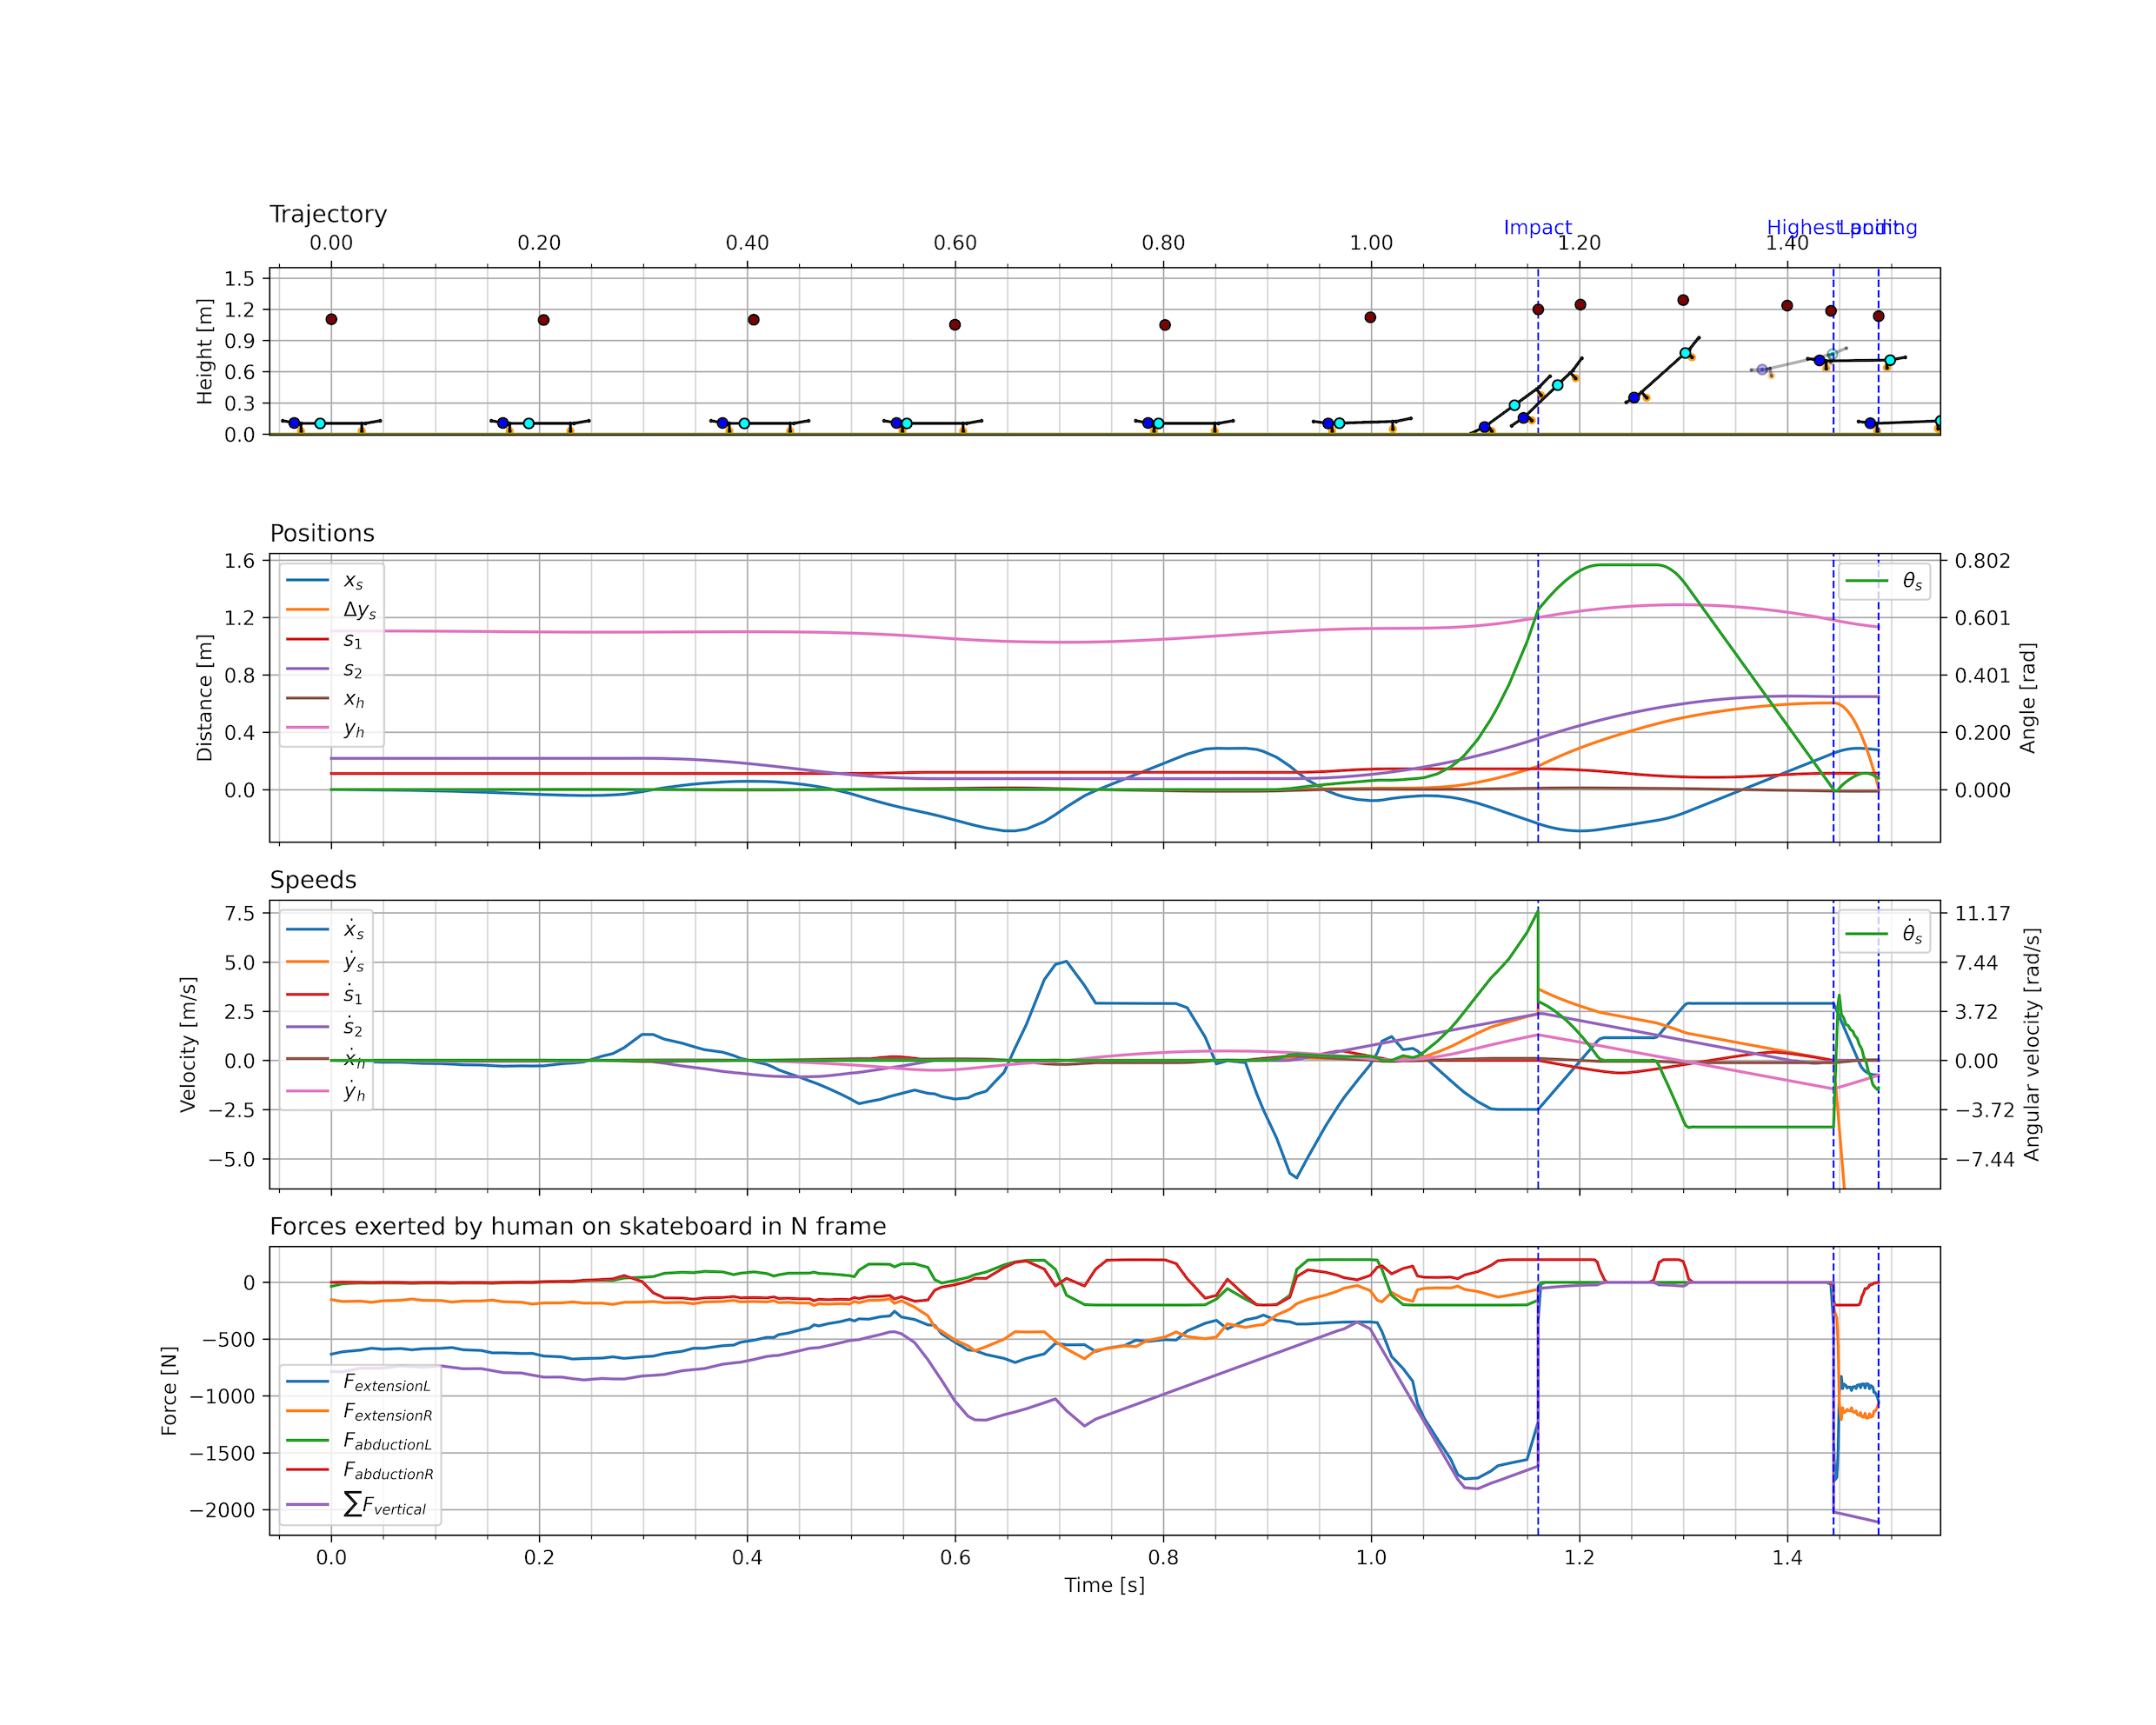
\includegraphics[trim={0cm 0cm 0cm 0cm},clip,width=0.8\textwidth]{figure/Results/data_longboard_init_longer_tail_optdpi600.png}}
    \newline
    \subfloat[All parameters no trucks]{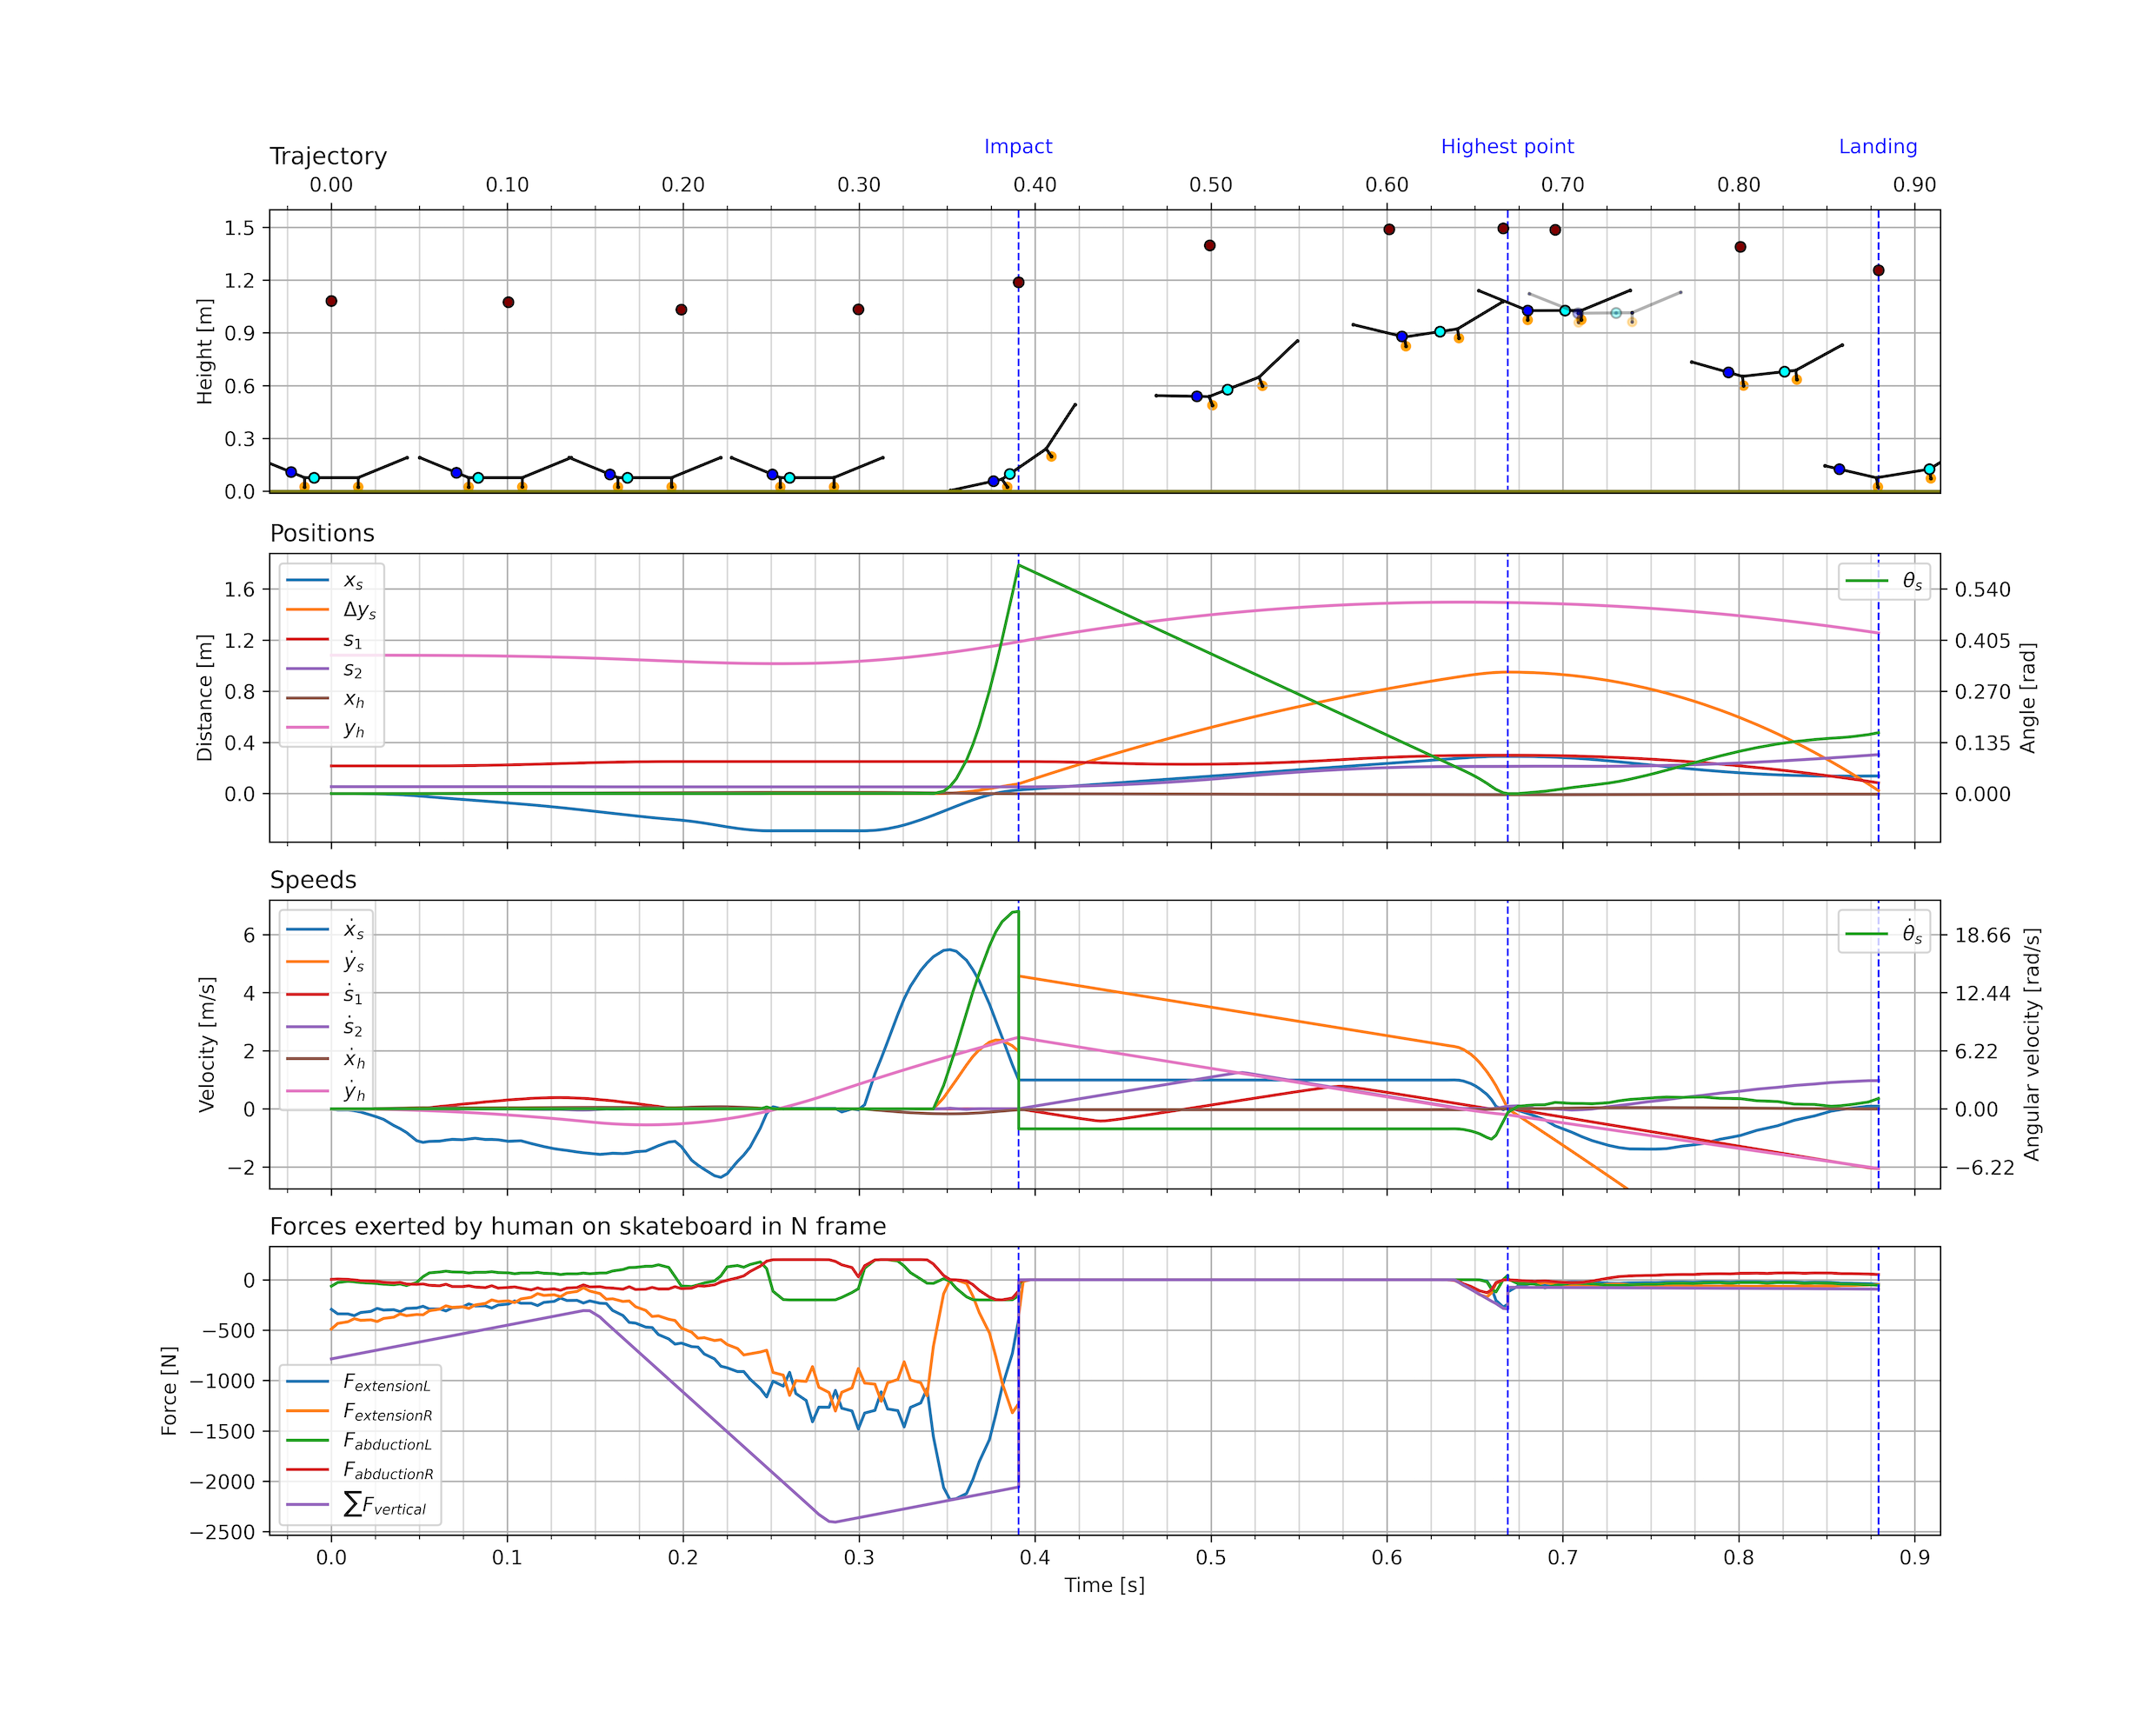
\includegraphics[trim={0cm 0cm 0cm 0cm},clip,width=0.8\textwidth]{figure/Results/data_notrrwdpi600.png}}
    \label{f_longboard}
    \caption{Longboard and `all except trucks' optimization results}
\end{figure*}

\begin{figure*}[b]    
    \subfloat[Plastic]{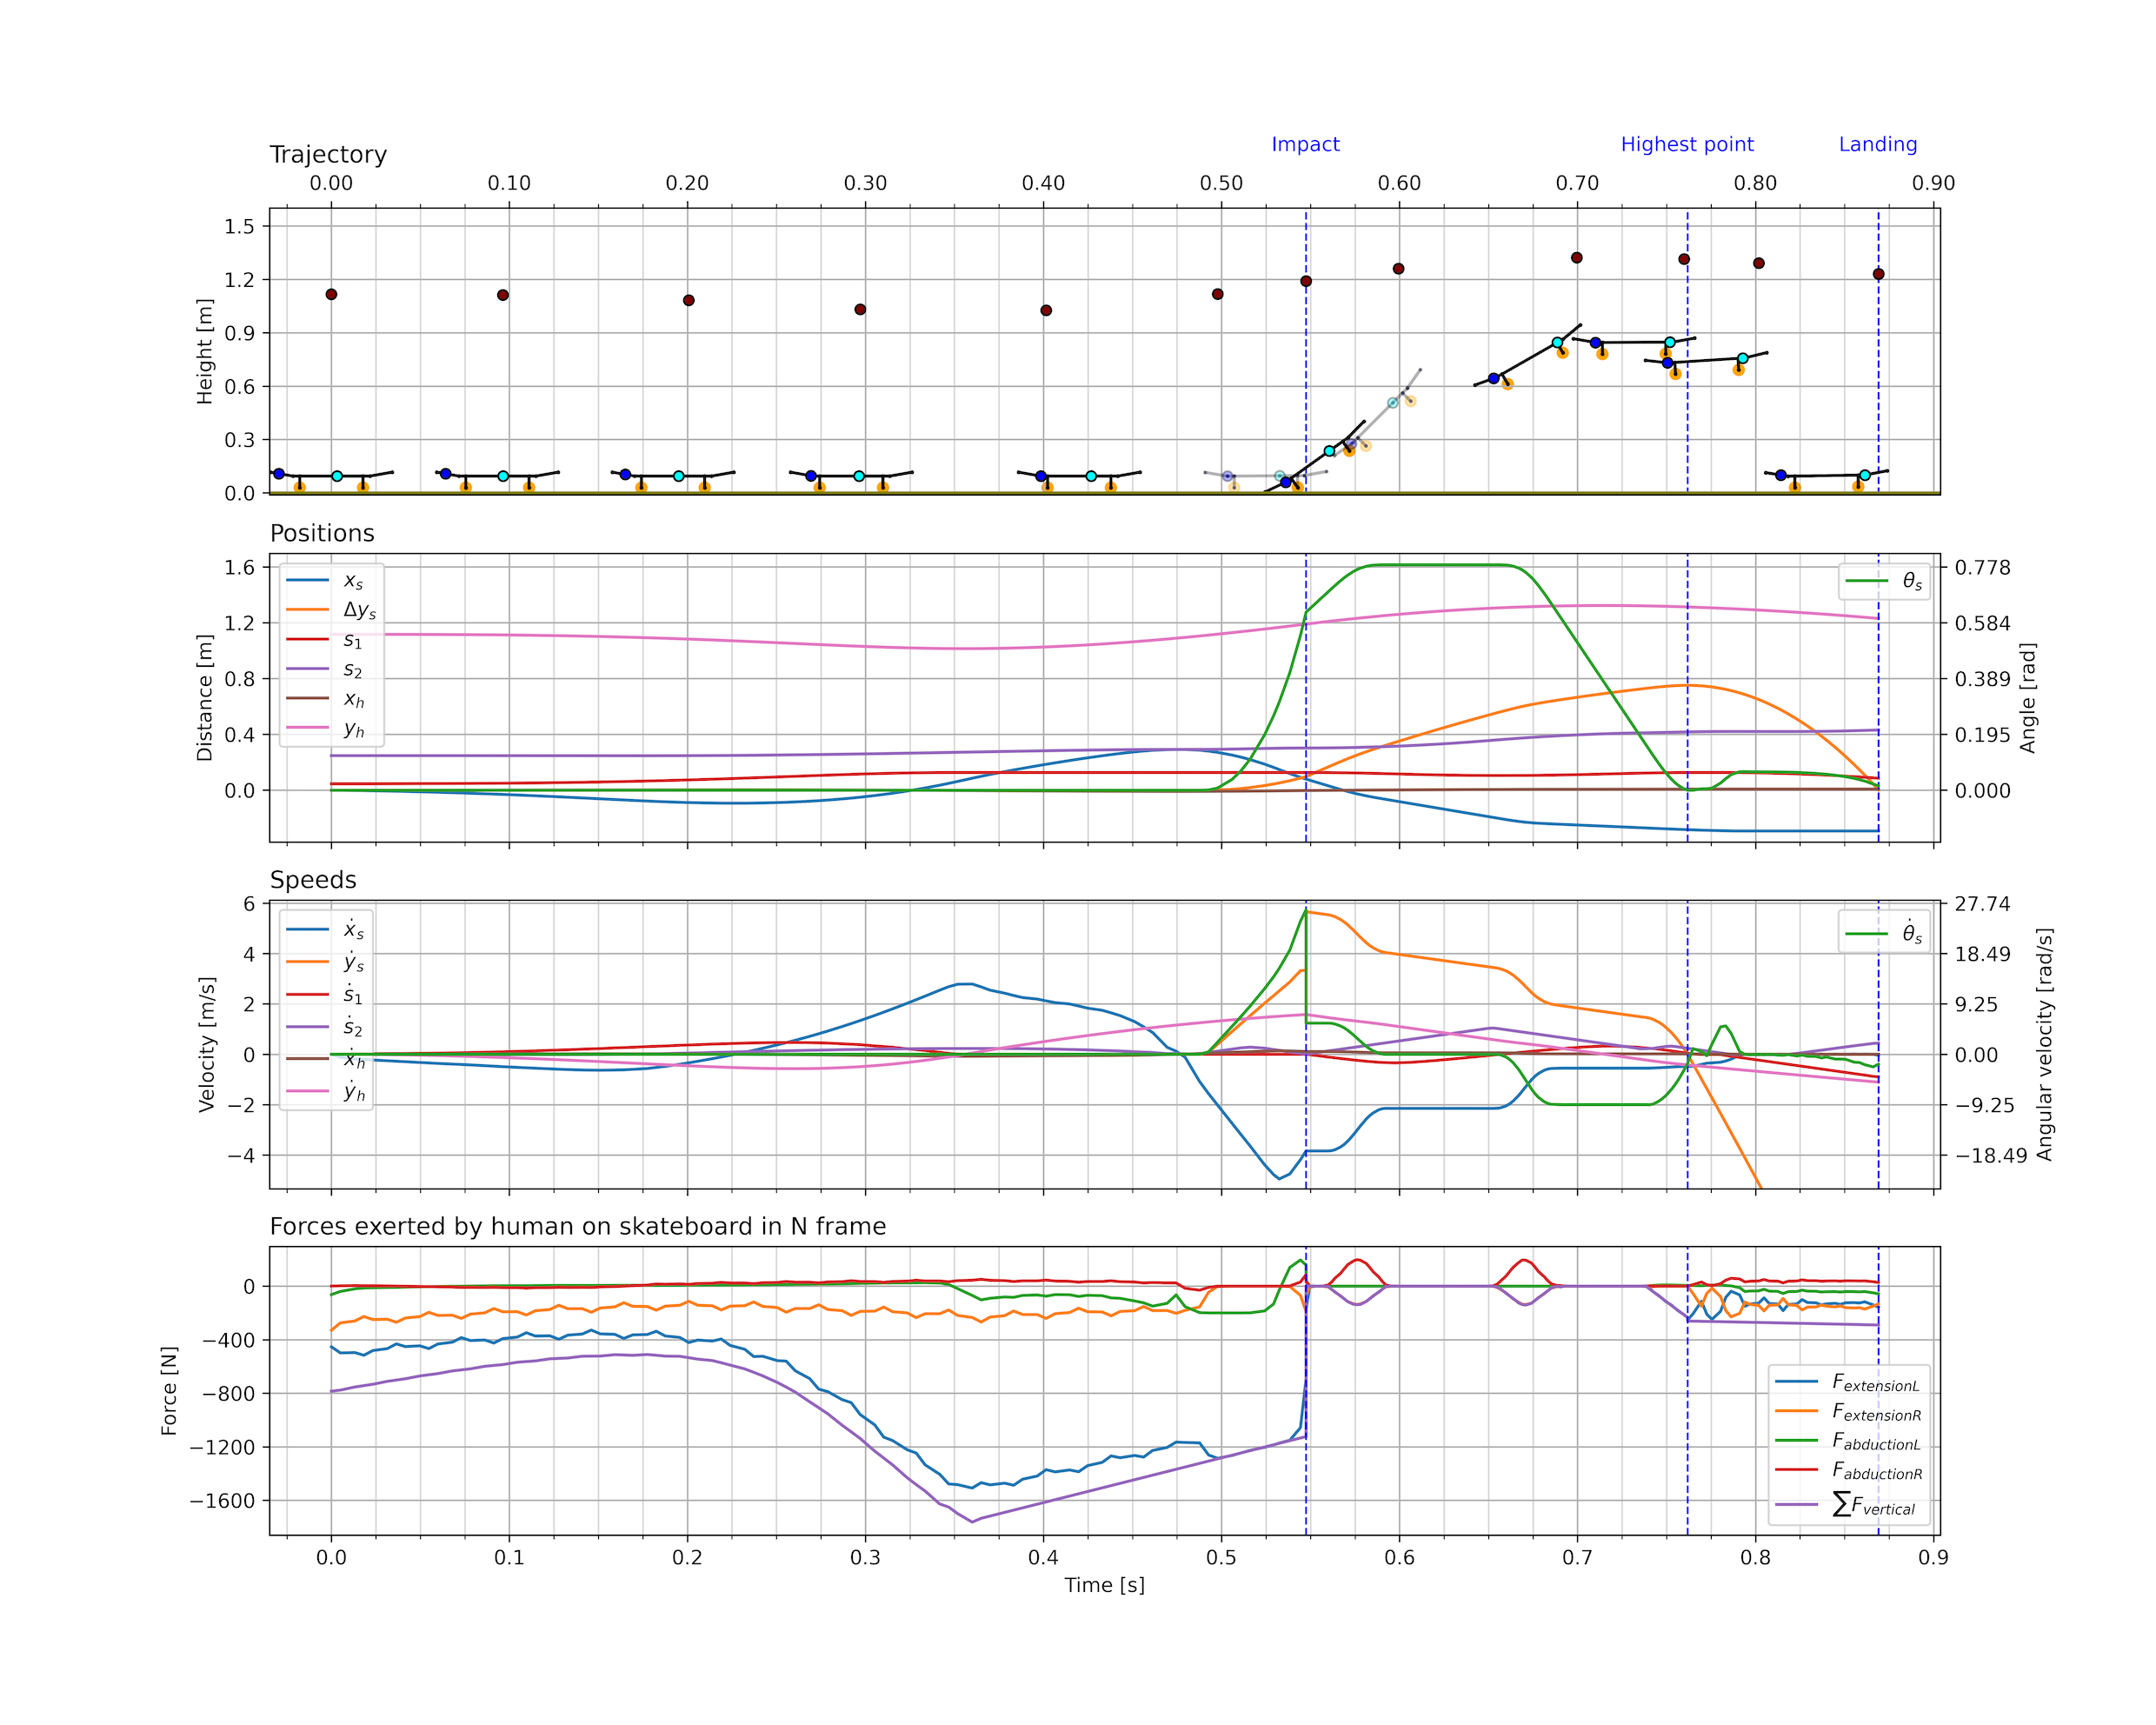
\includegraphics[trim={0cm 0cm 0cm 0cm},clip,width=0.8\textwidth]{figure/Results/data_penny_02dpi600.png}}
    \newline
    \subfloat[Griptape]{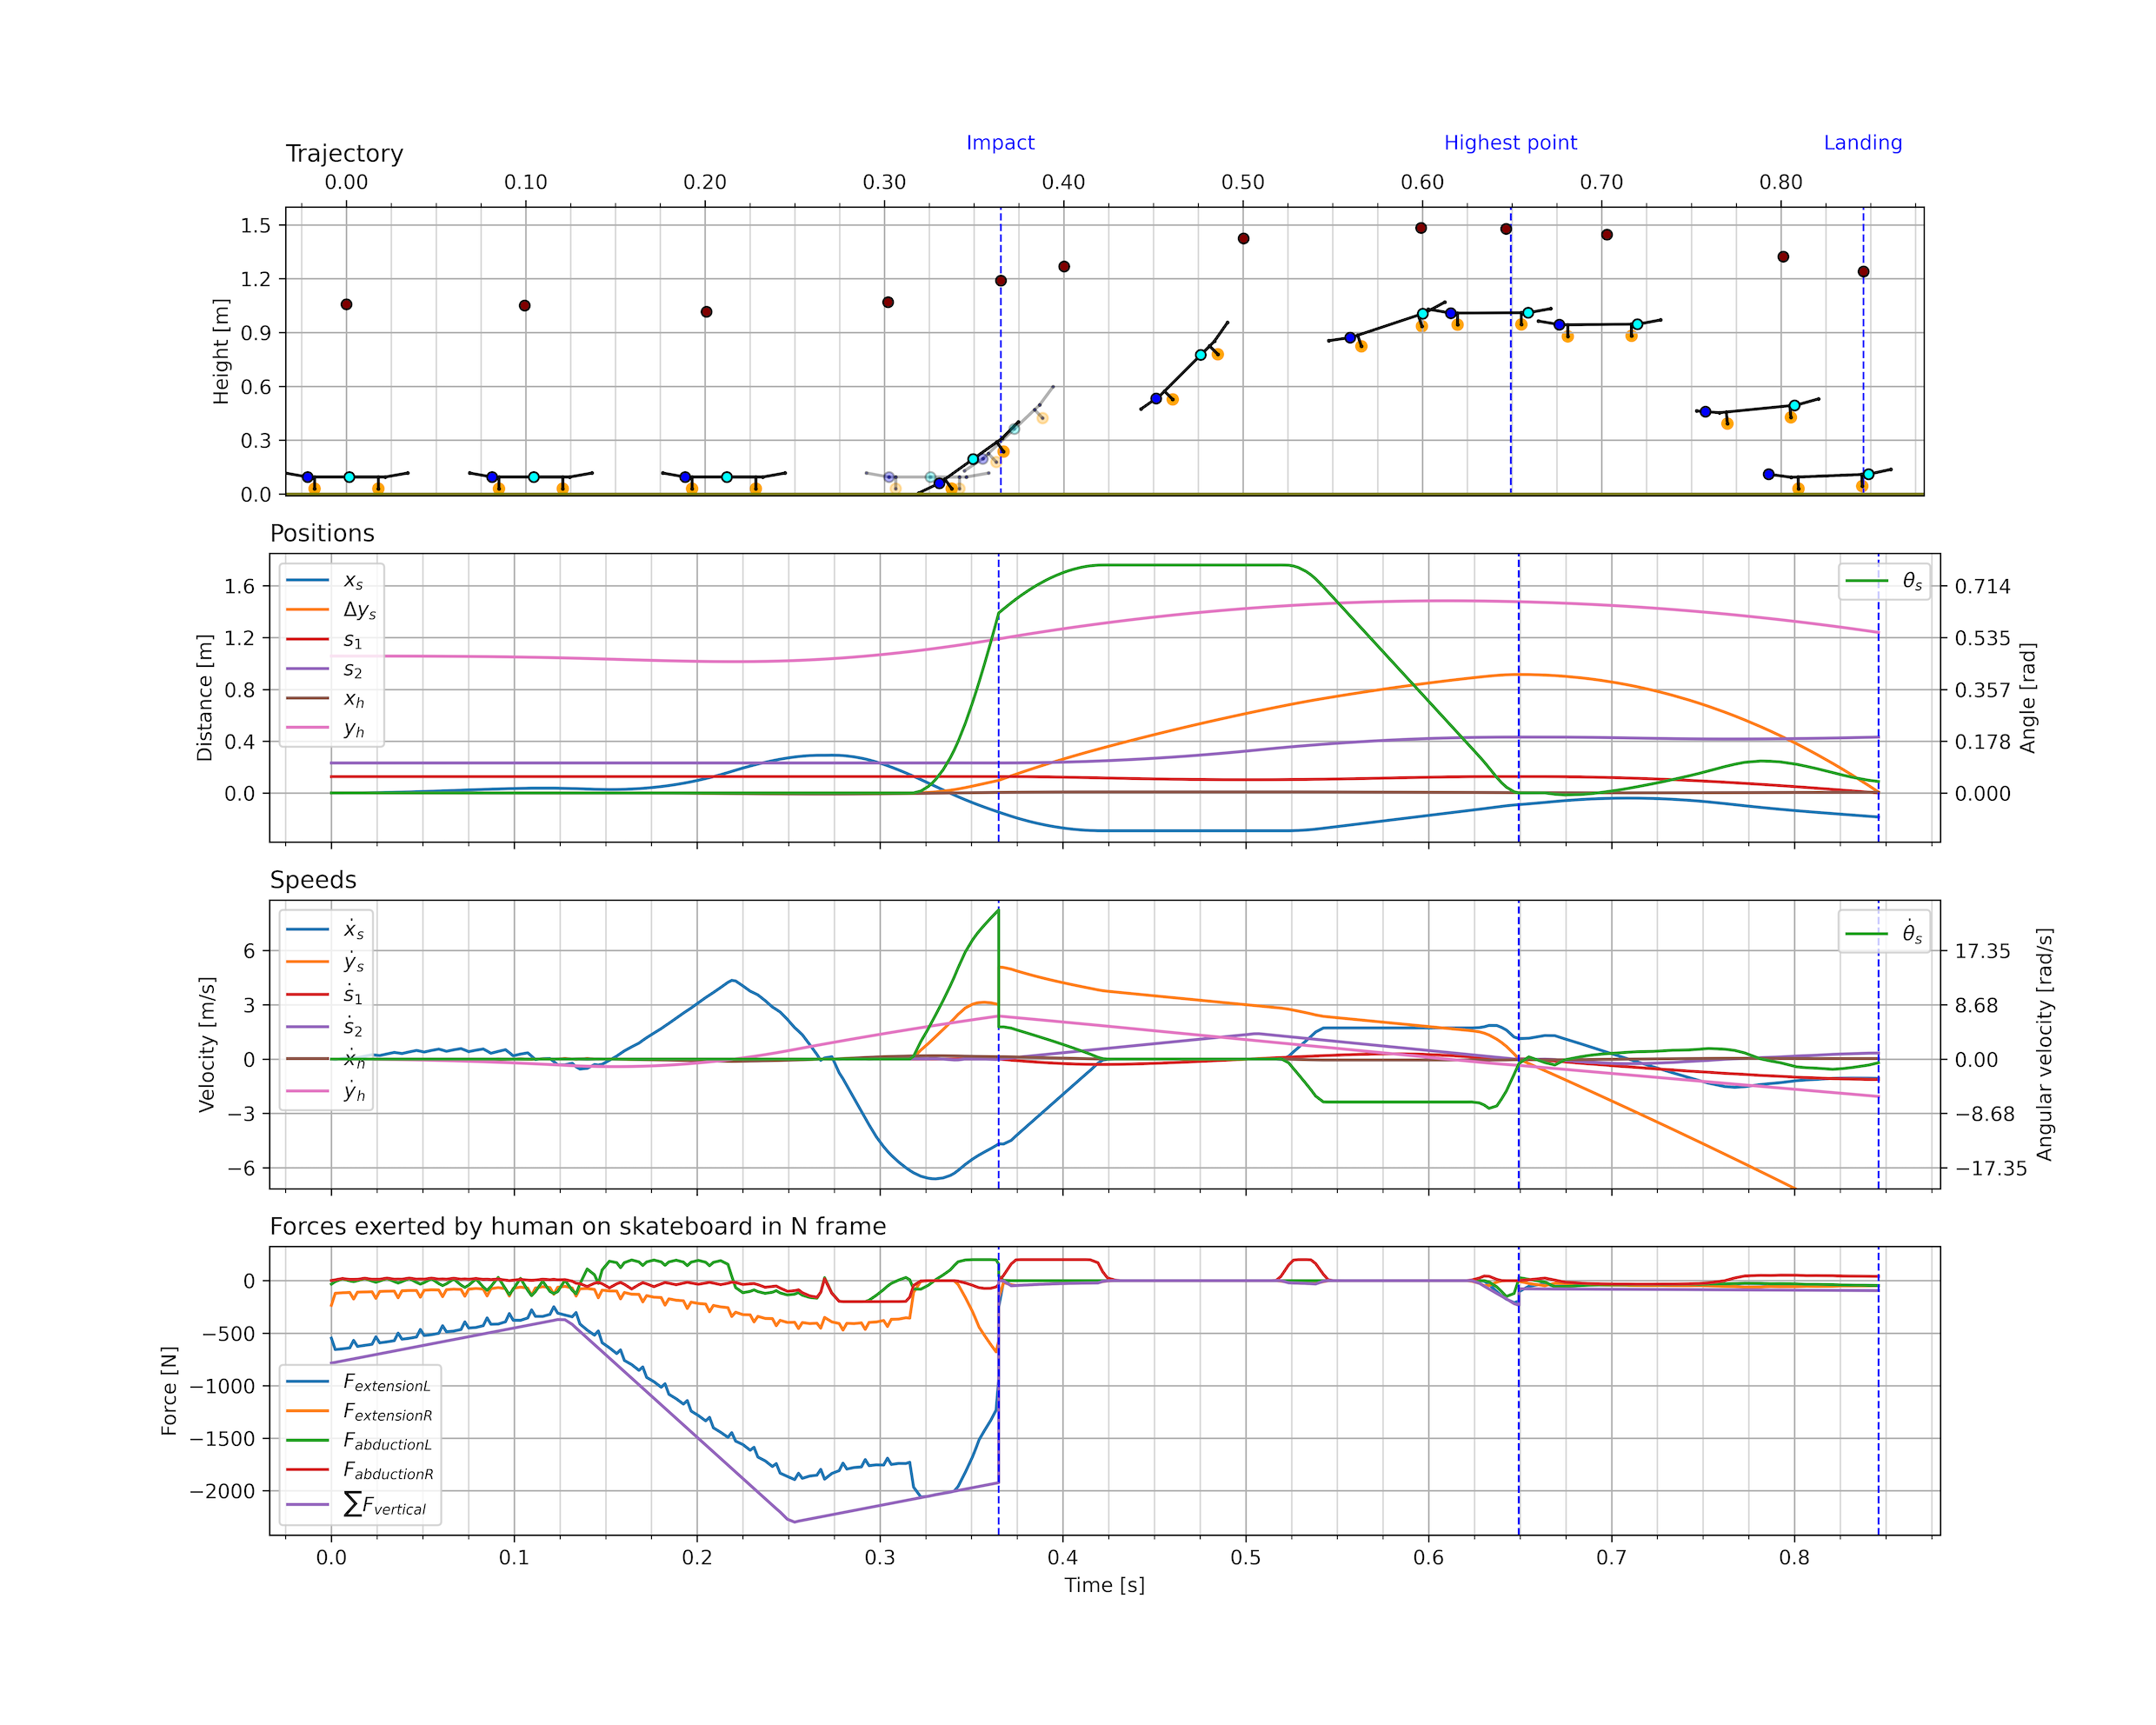
\includegraphics[trim={0cm 0cm 0cm 0cm},clip,width=0.8\textwidth]{figure/Results/data_penny_08dpi600.png}}
    \caption{Penny boards optimization results}    
\end{figure*}

\begin{figure*}[b]    
    \subfloat[Wheel radius]{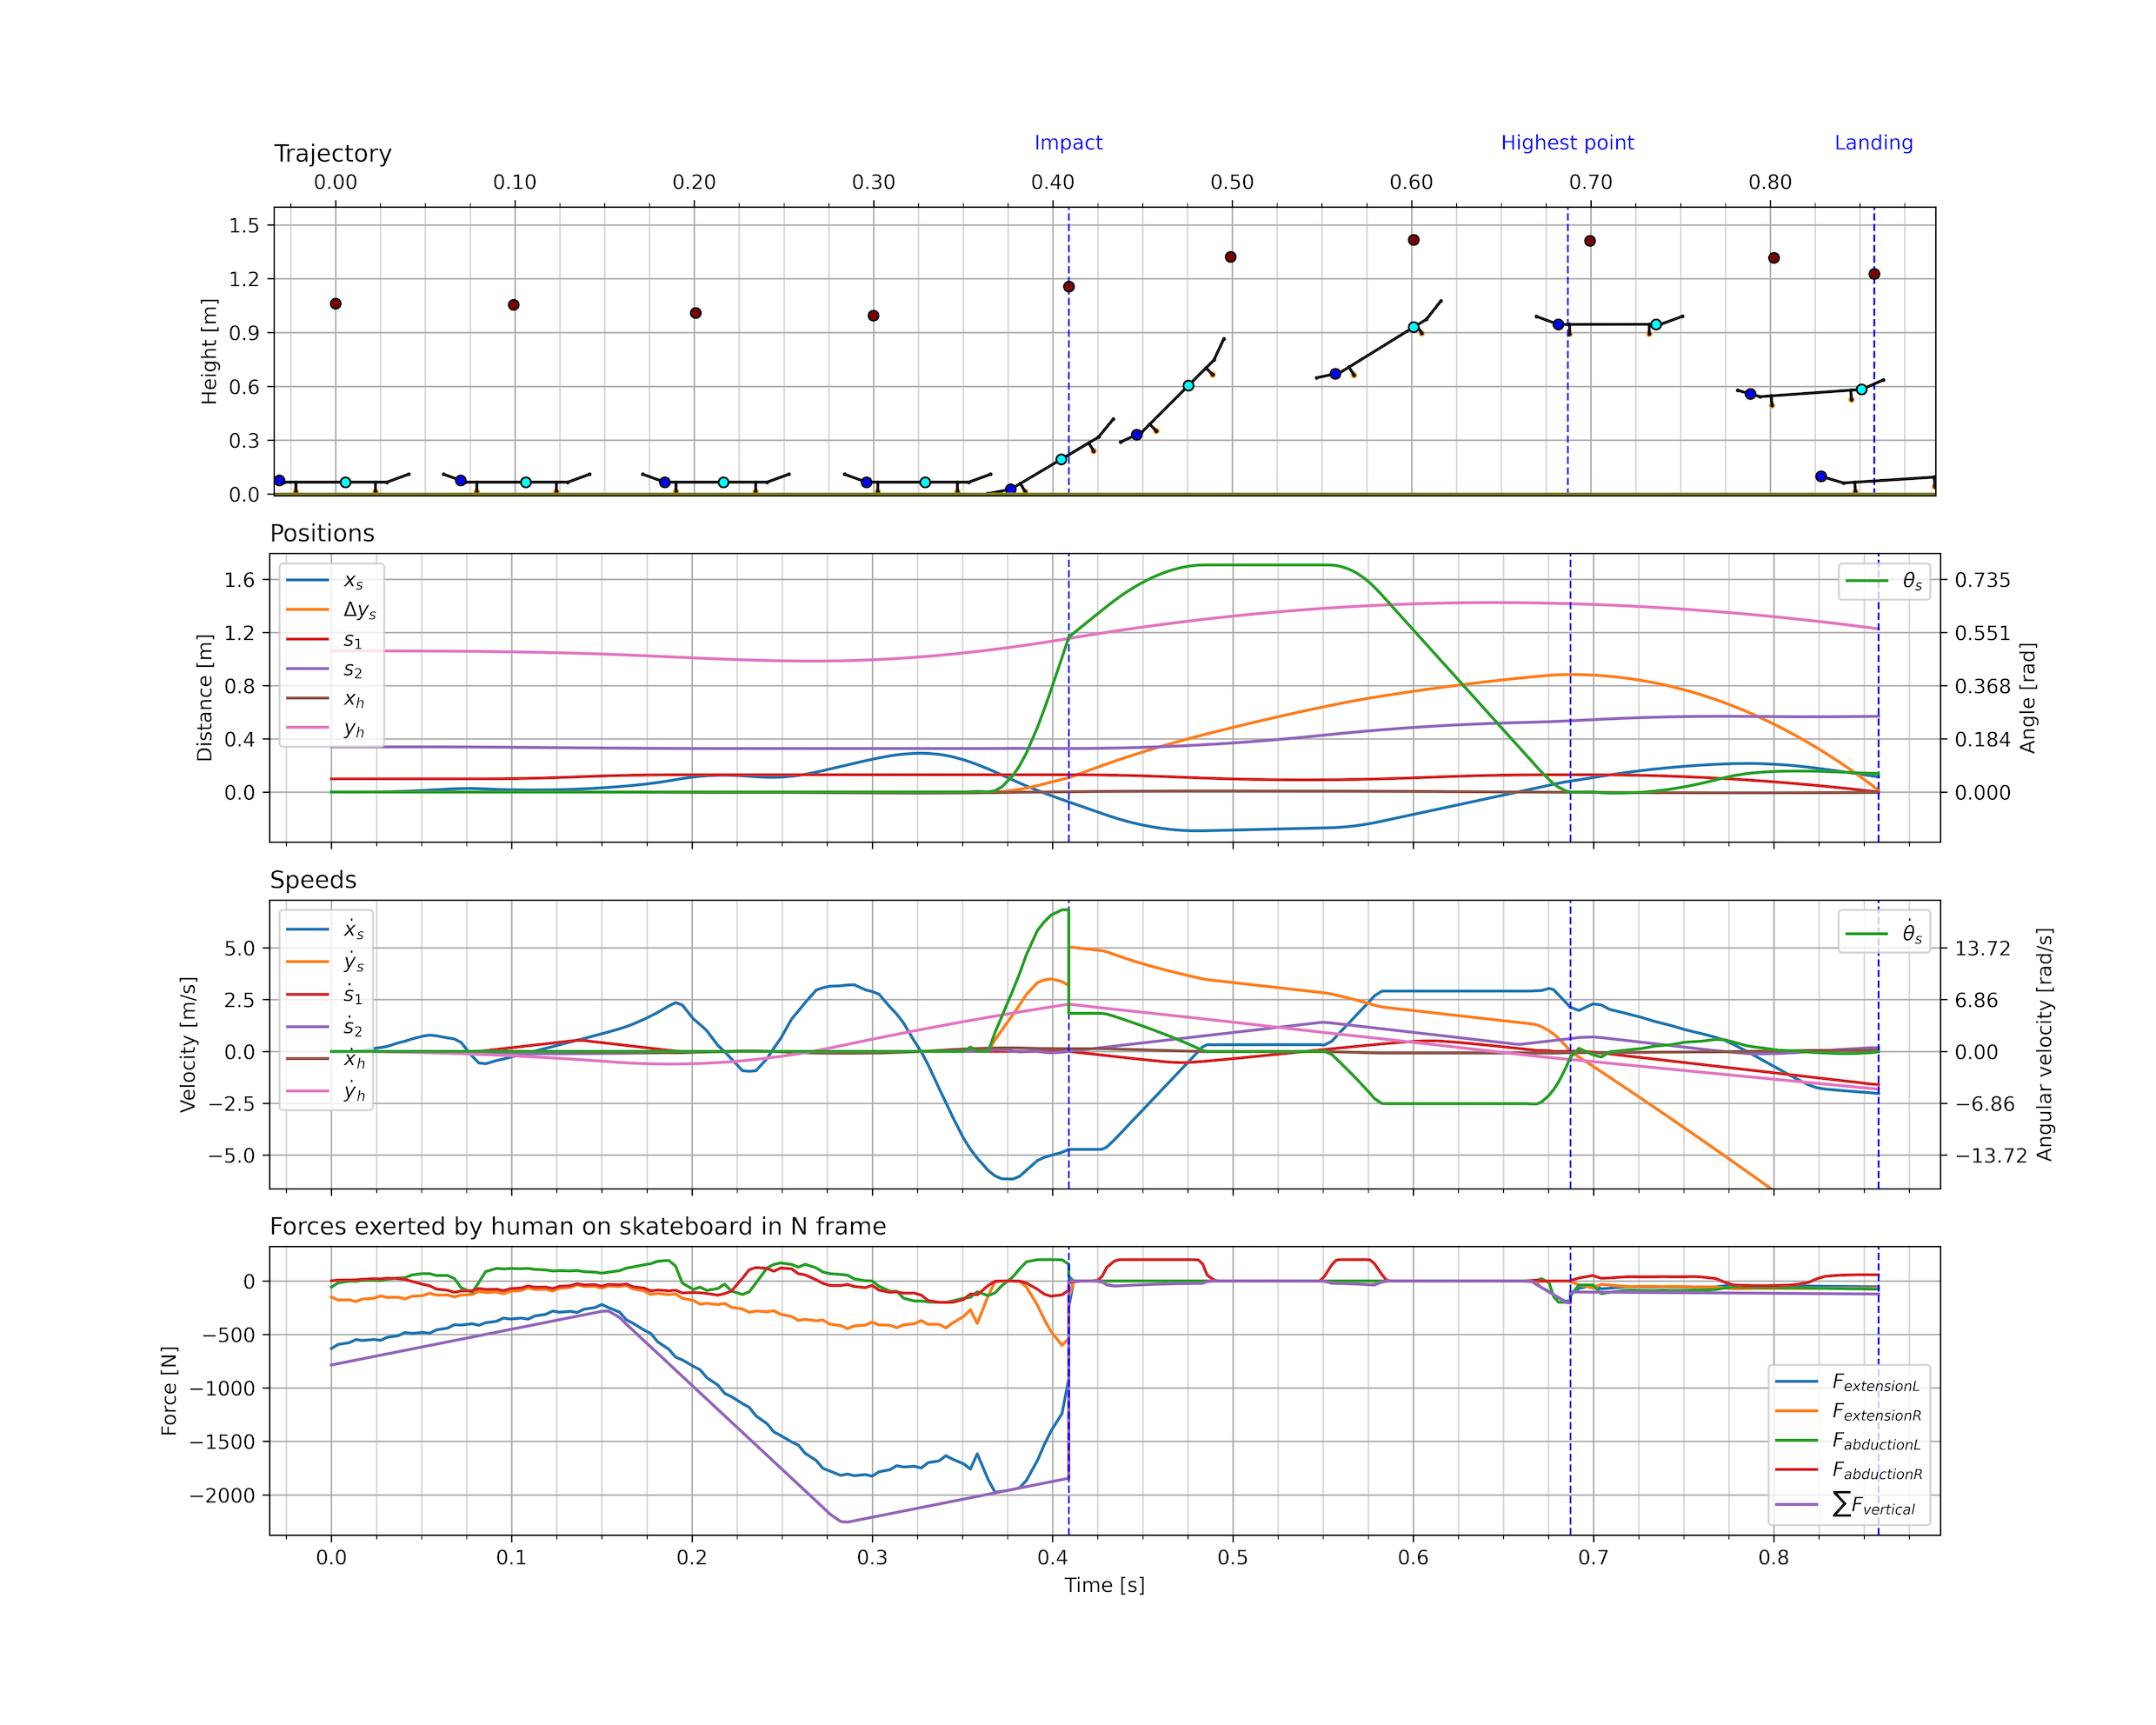
\includegraphics[trim={0cm 0cm 0cm 0cm},clip,width=0.8\textwidth]{figure/Results/data_r_wdpi600.png}}
    \newline
    \subfloat[Truck height]{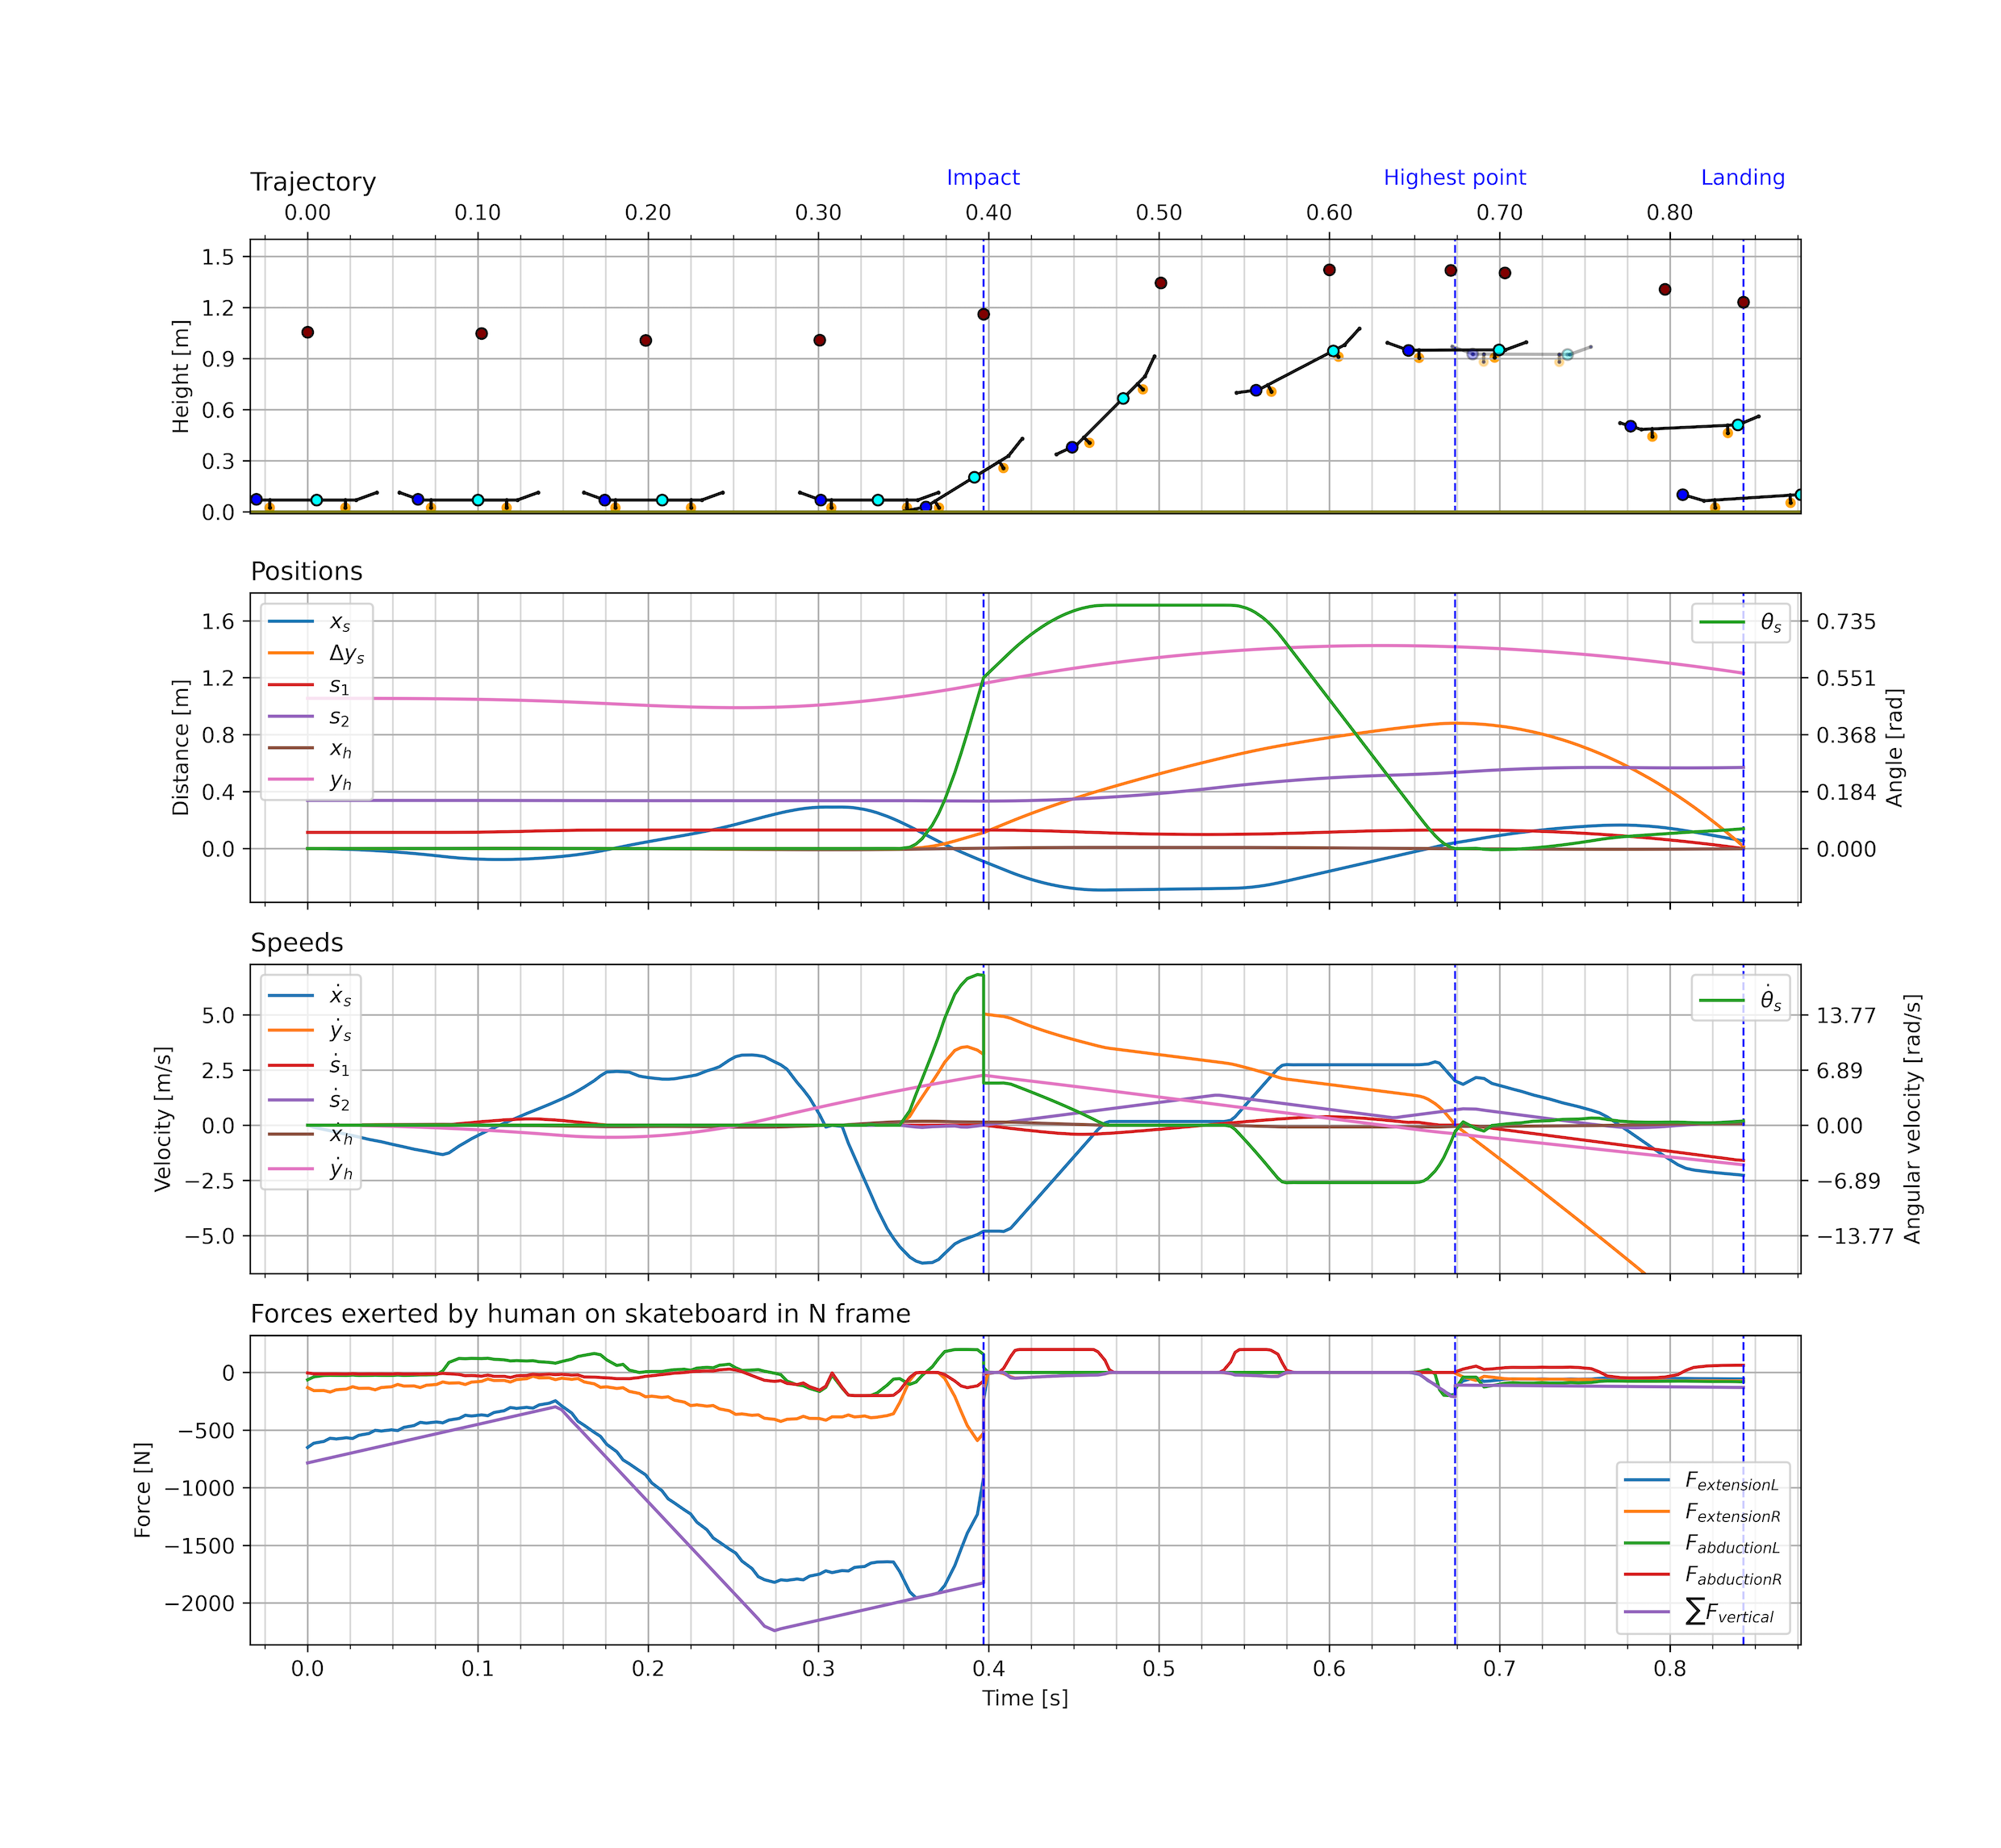
\includegraphics[trim={0cm 0cm 0cm 0cm},clip,width=0.8\textwidth]{figure/Results/data_d_trdpi600.png}}
    \caption{Wheel radius and truck height optimization results}    
\end{figure*}

% \begin{figure*}[b]    
%     \subfloat[Wheel radius]{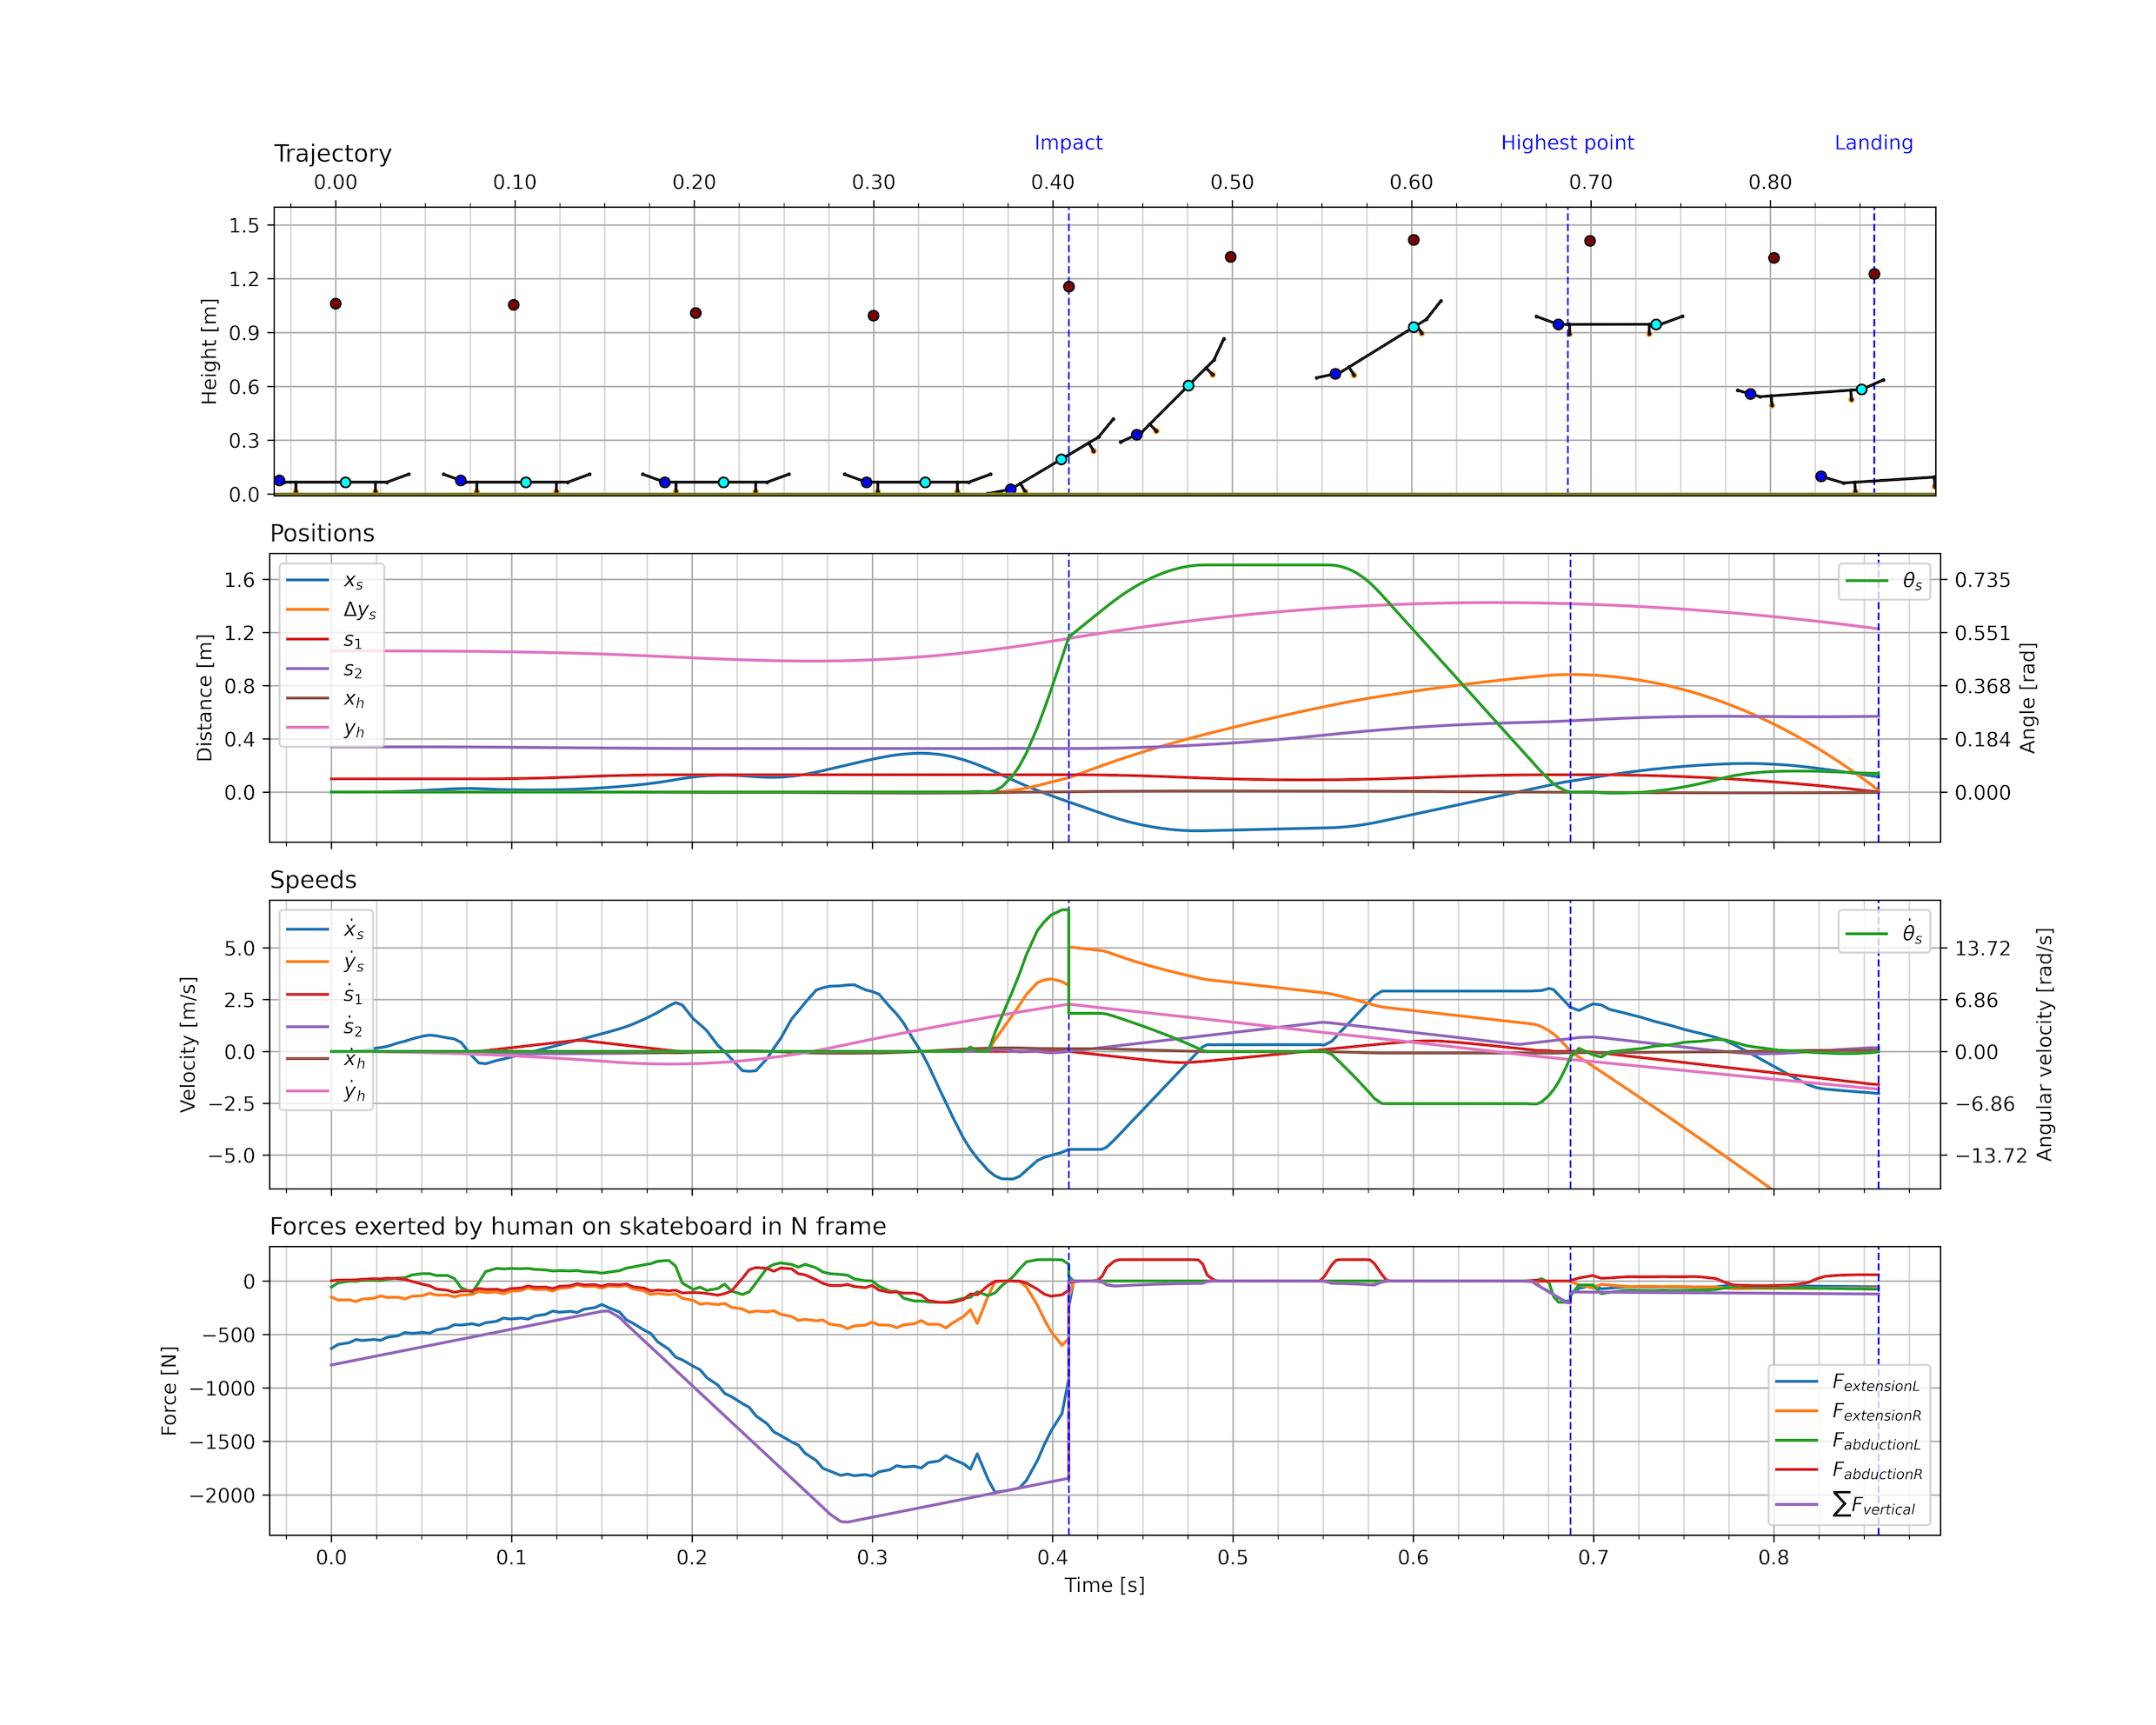
\includegraphics[trim={0cm 0cm 0cm 0cm},clip,width=0.8\textwidth]{figure/Results/data_r_wdpi600.png}}
%     \newline
%     \subfloat[Truck height]{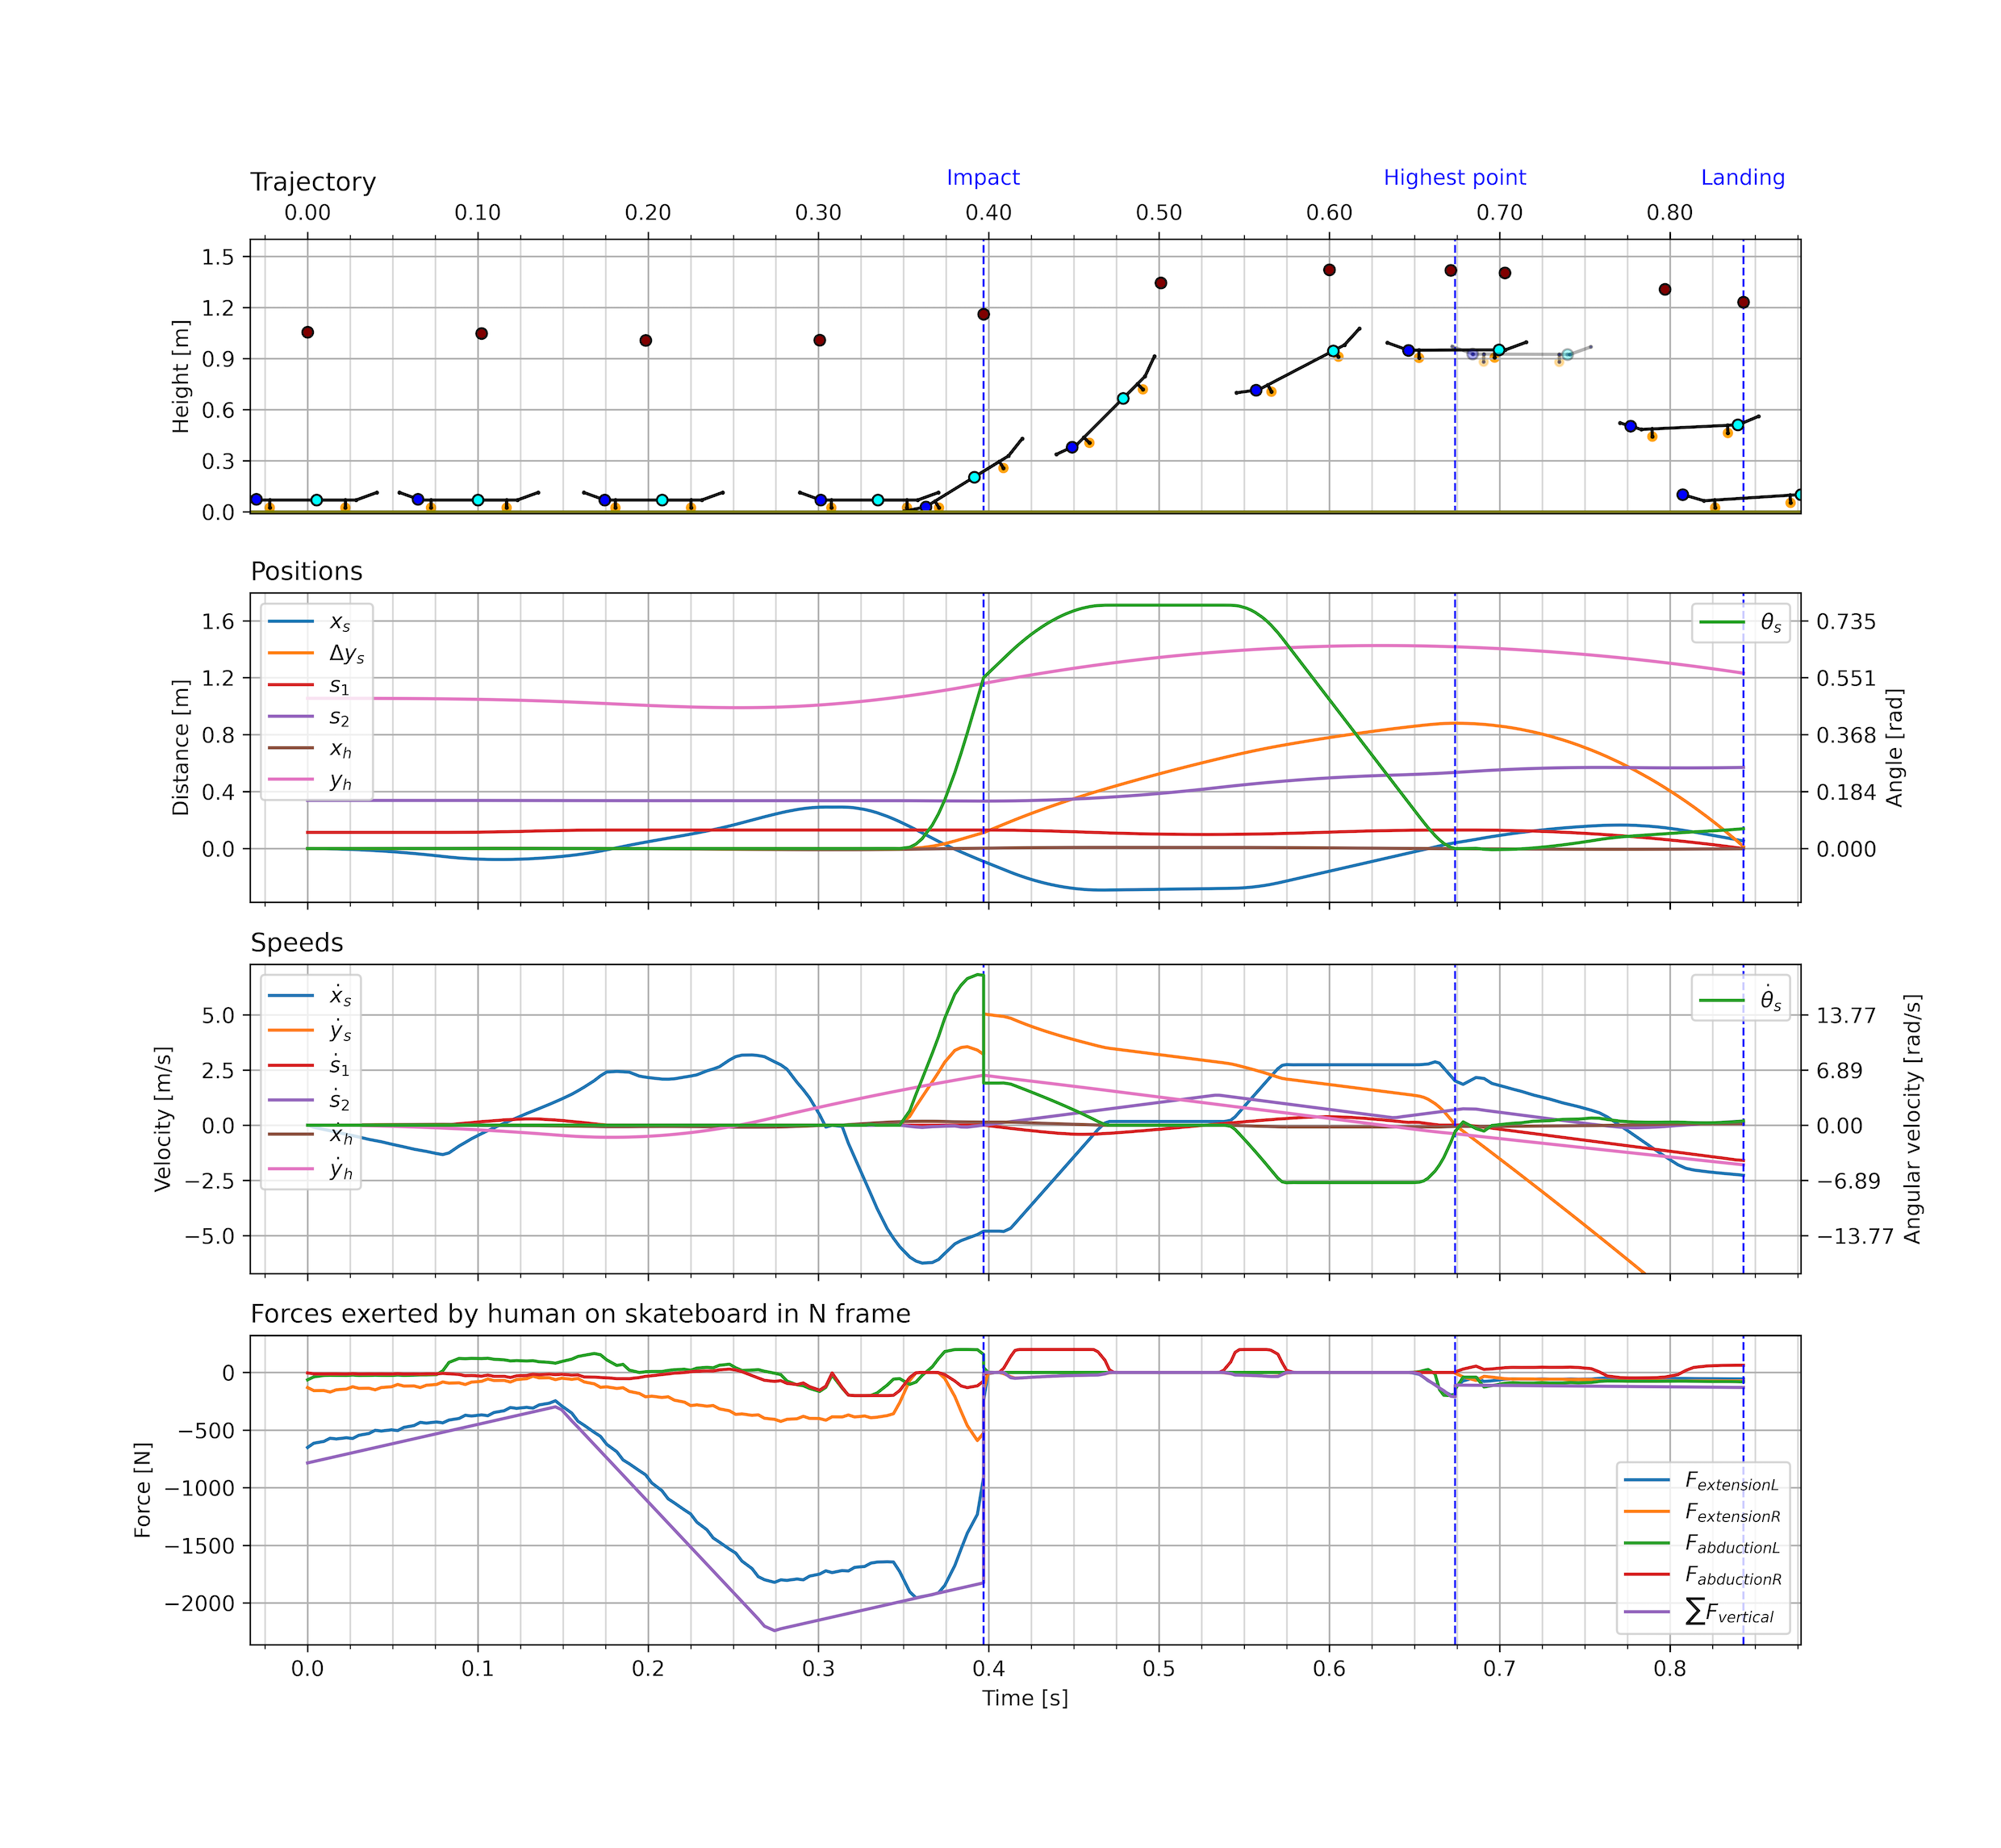
\includegraphics[trim={0cm 0cm 0cm 0cm},clip,width=0.8\textwidth]{figure/Results/data_d_trdpi600.png}}
%     \caption{Single parameter optimization}    
% \end{figure*}

\begin{figure*}[b]    
    \subfloat[Deck length]{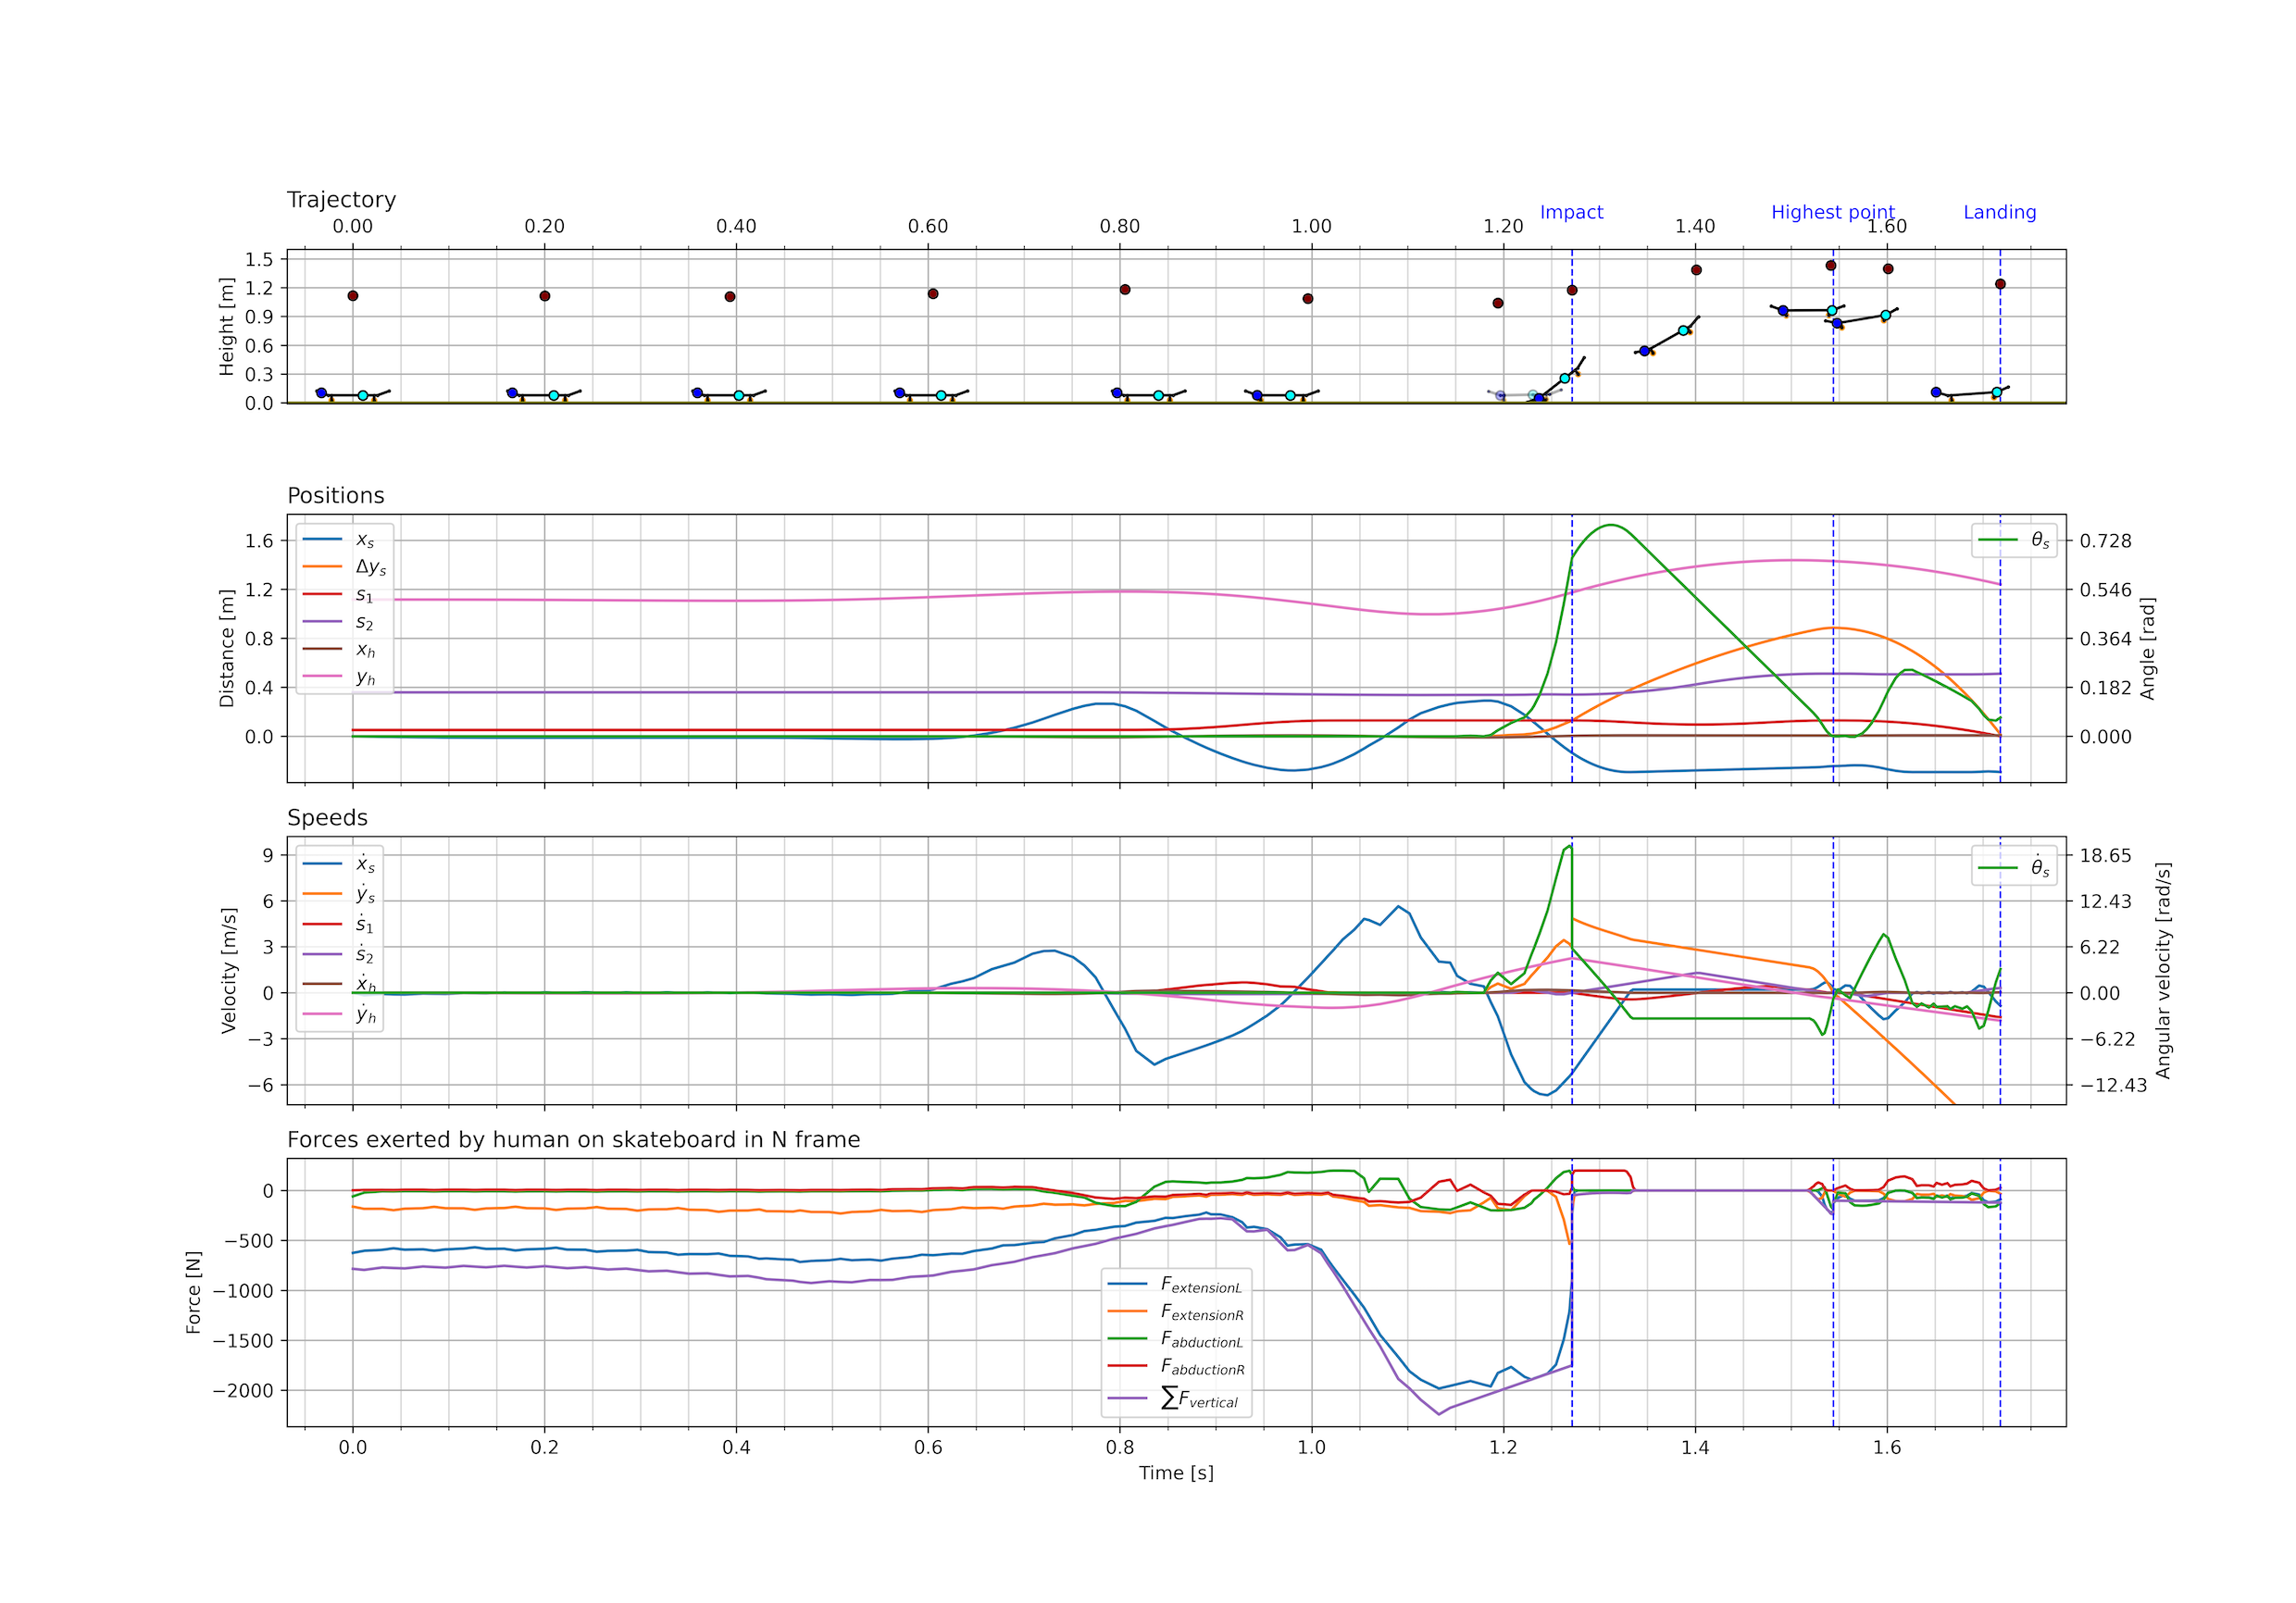
\includegraphics[trim={0cm 0cm 0cm 0cm},clip,width=0.8\textwidth]{figure/Results/data_l_fdpi600.png}}
    \newline
    \subfloat[Tail length]{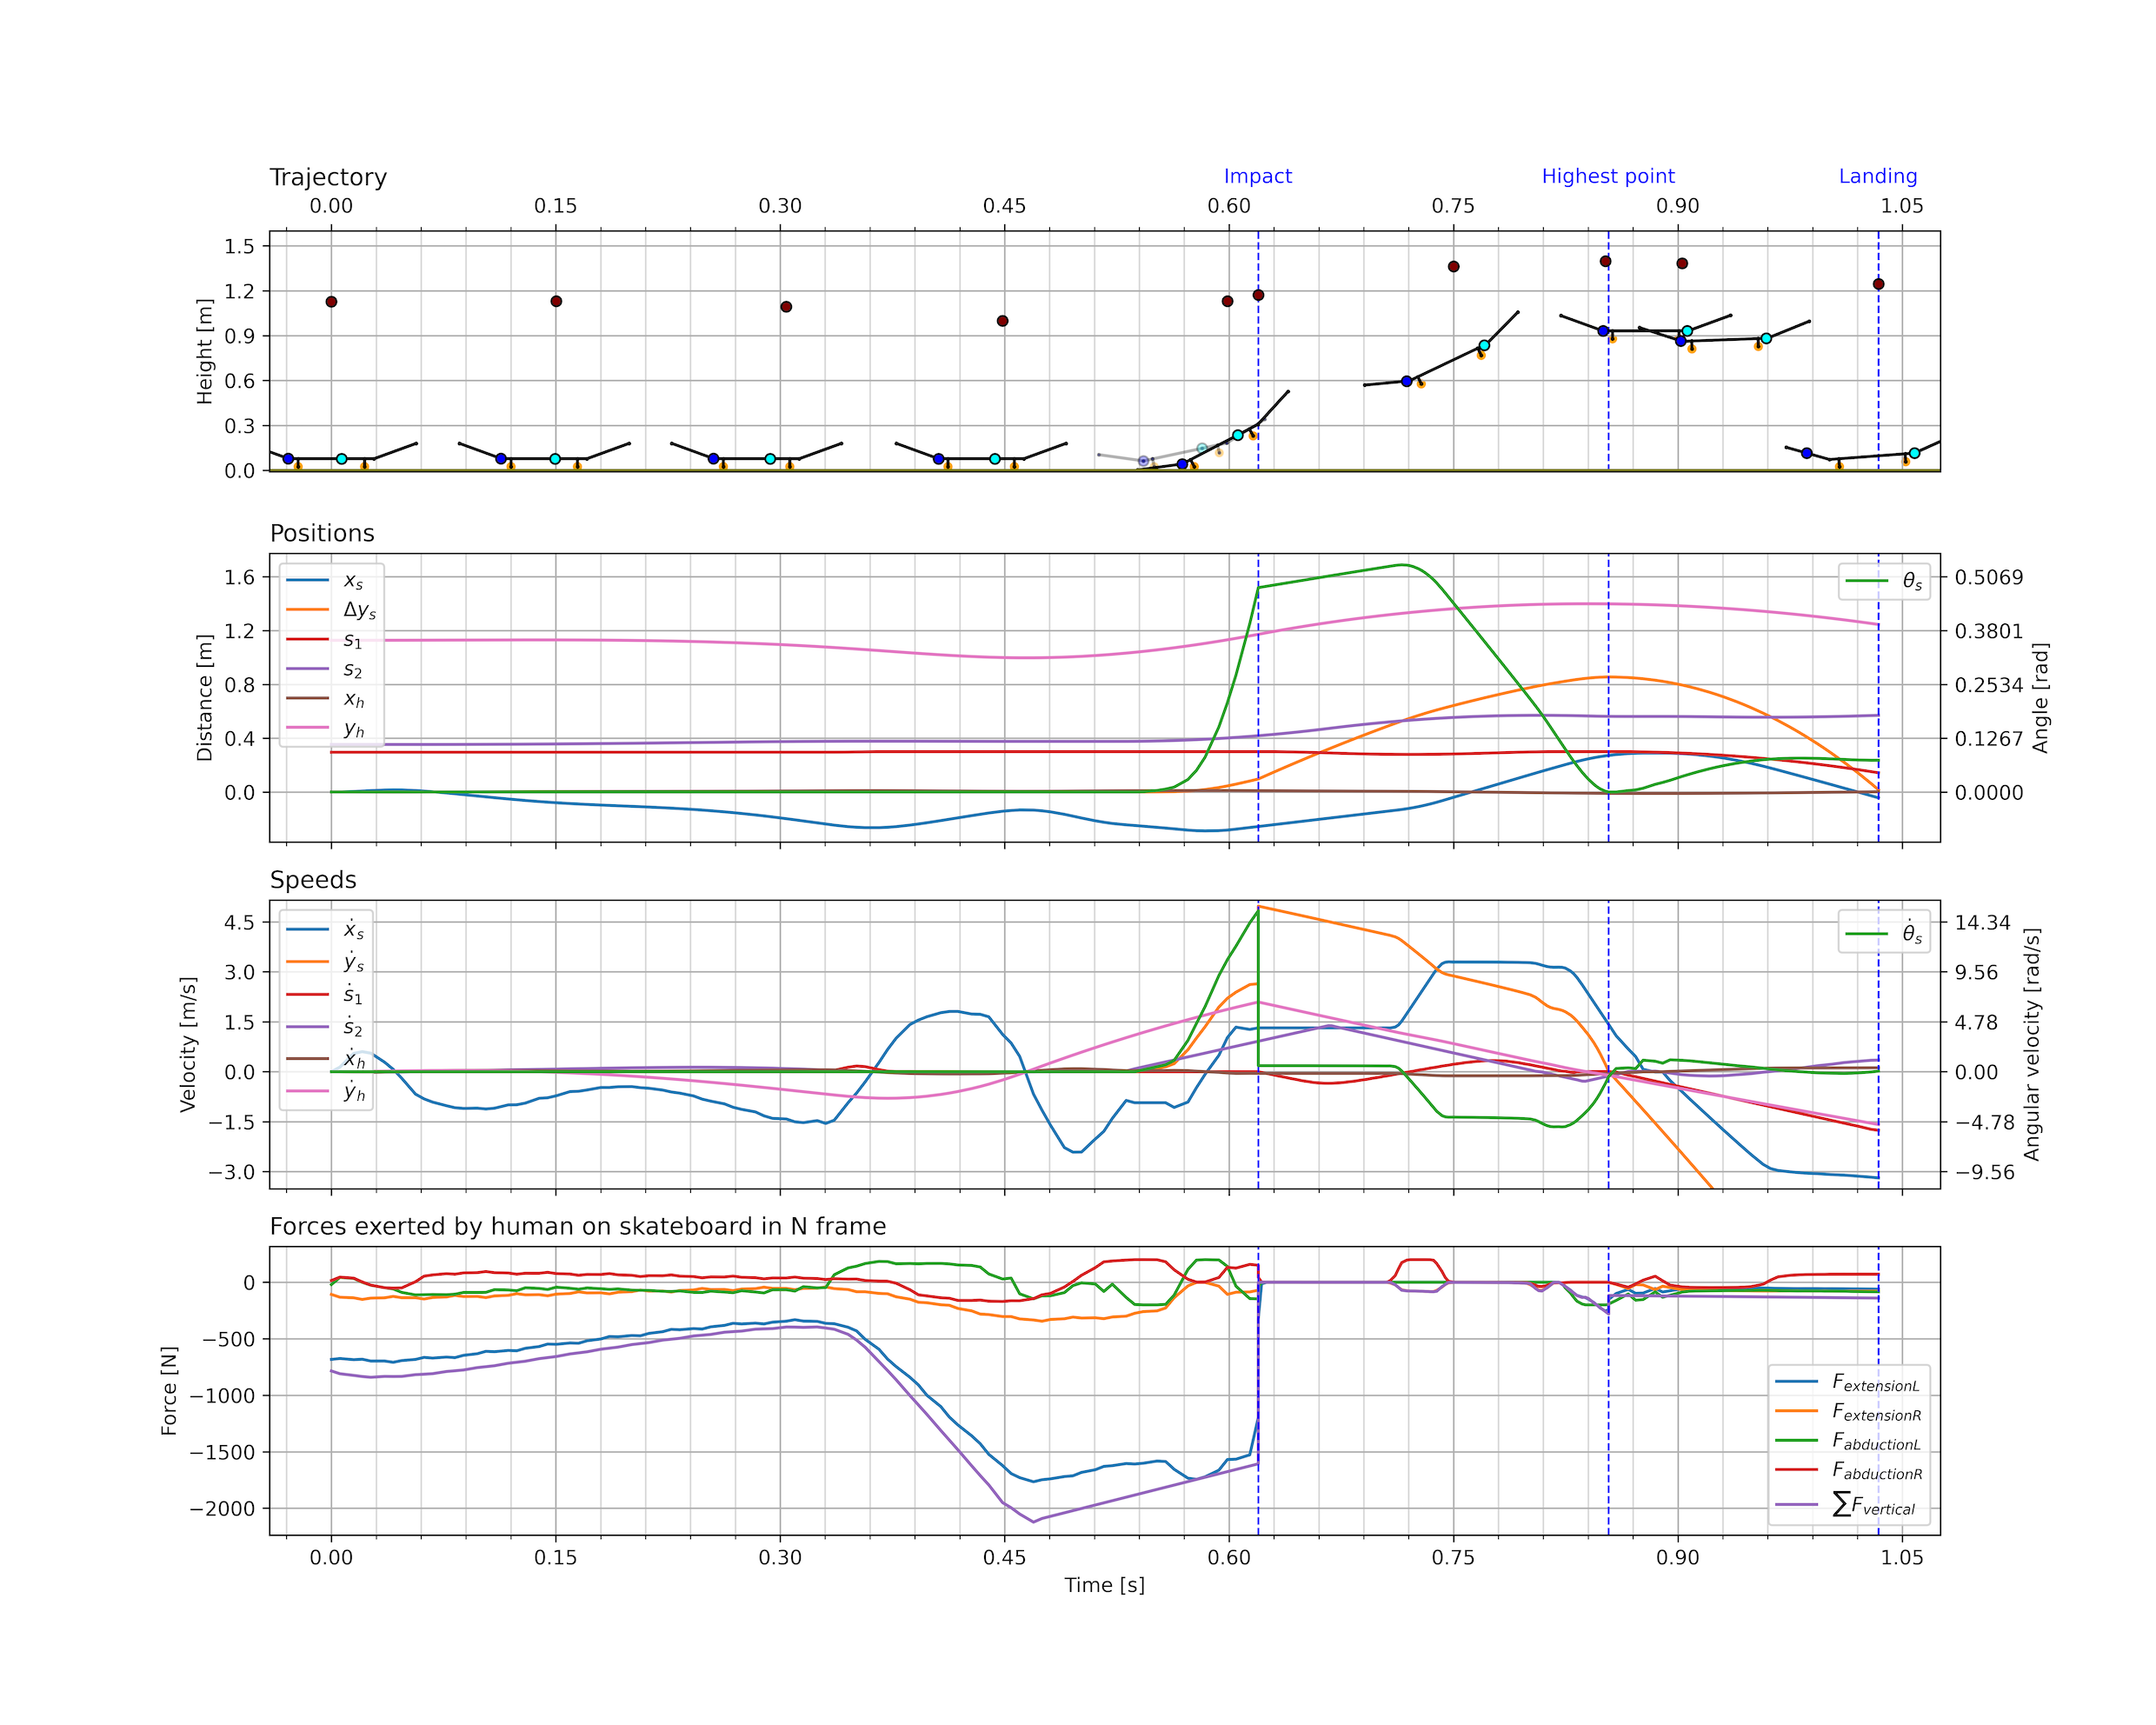
\includegraphics[trim={0cm 0cm 0cm 0cm},clip,width=0.8\textwidth]{figure/Results/data_l_tdpi600.png}}
    \caption{Deck length and tail length optimization results}    
\end{figure*}

\begin{figure*}[b]    
    \subfloat[Tail inclination]{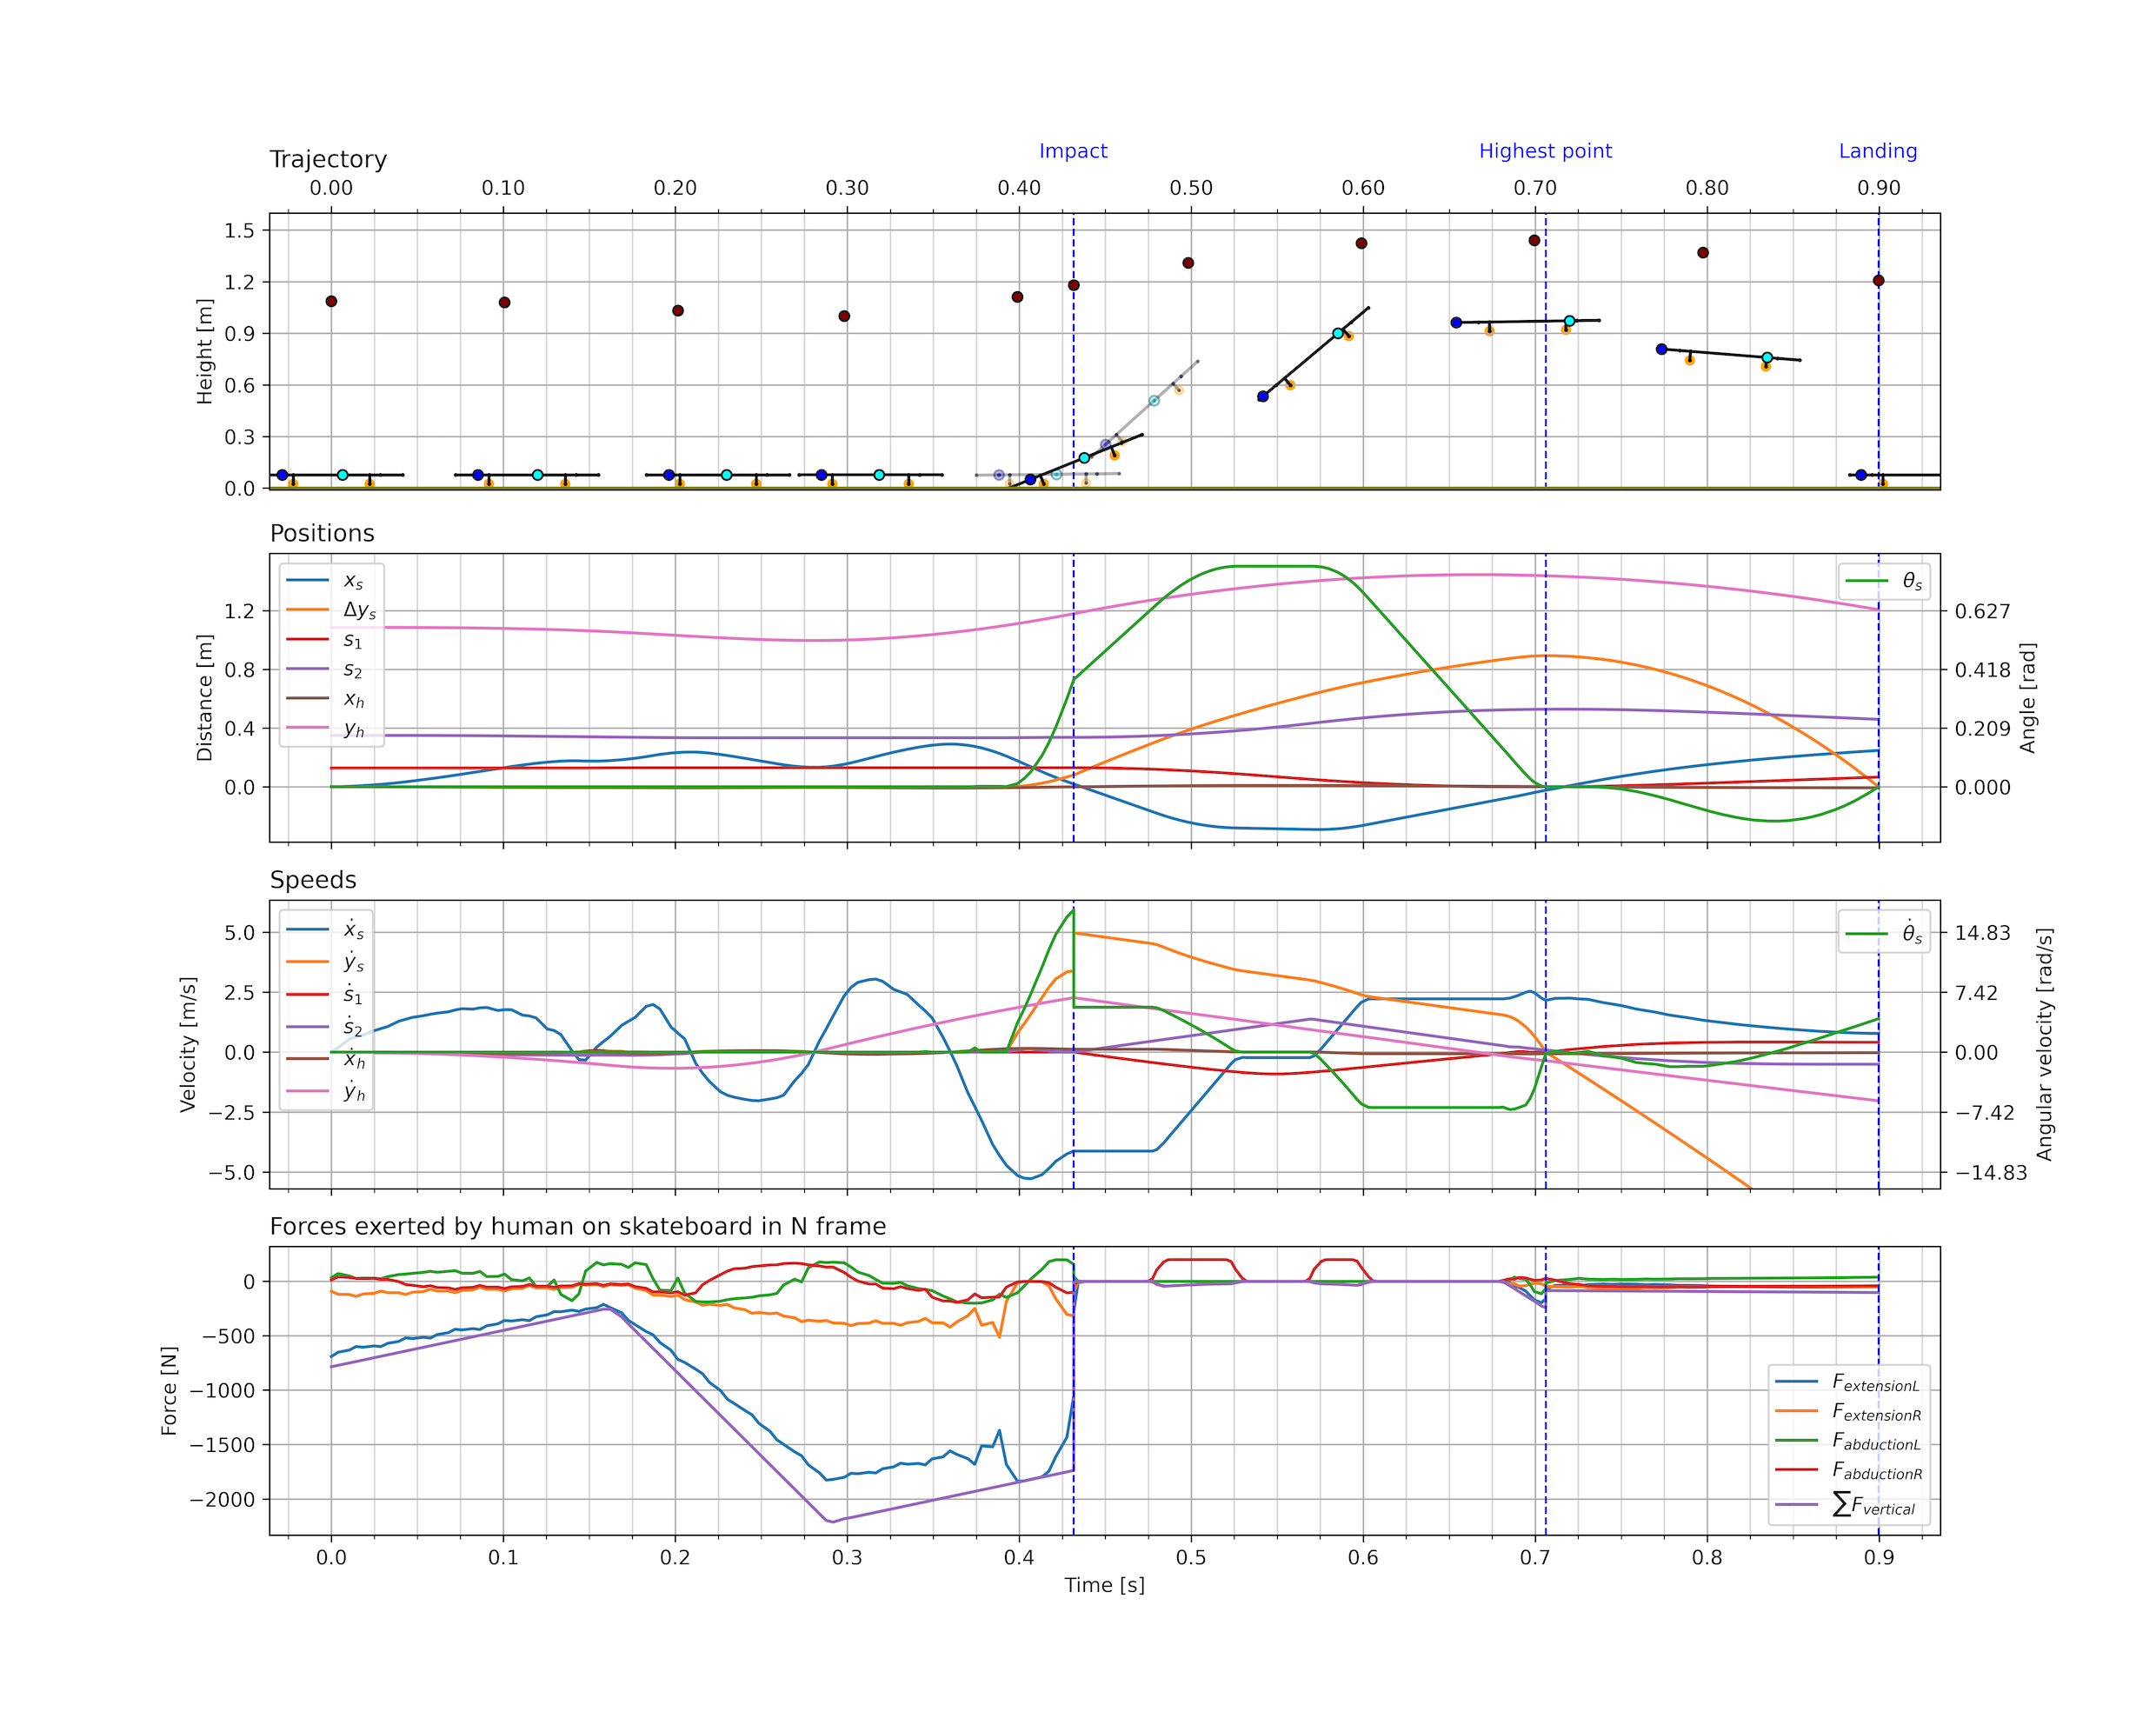
\includegraphics[trim={0cm 0cm 0cm 0cm},clip,width=0.8\textwidth]{figure/Results/data_phidpi600.png}}
    \newline
    \subfloat[All parameters]{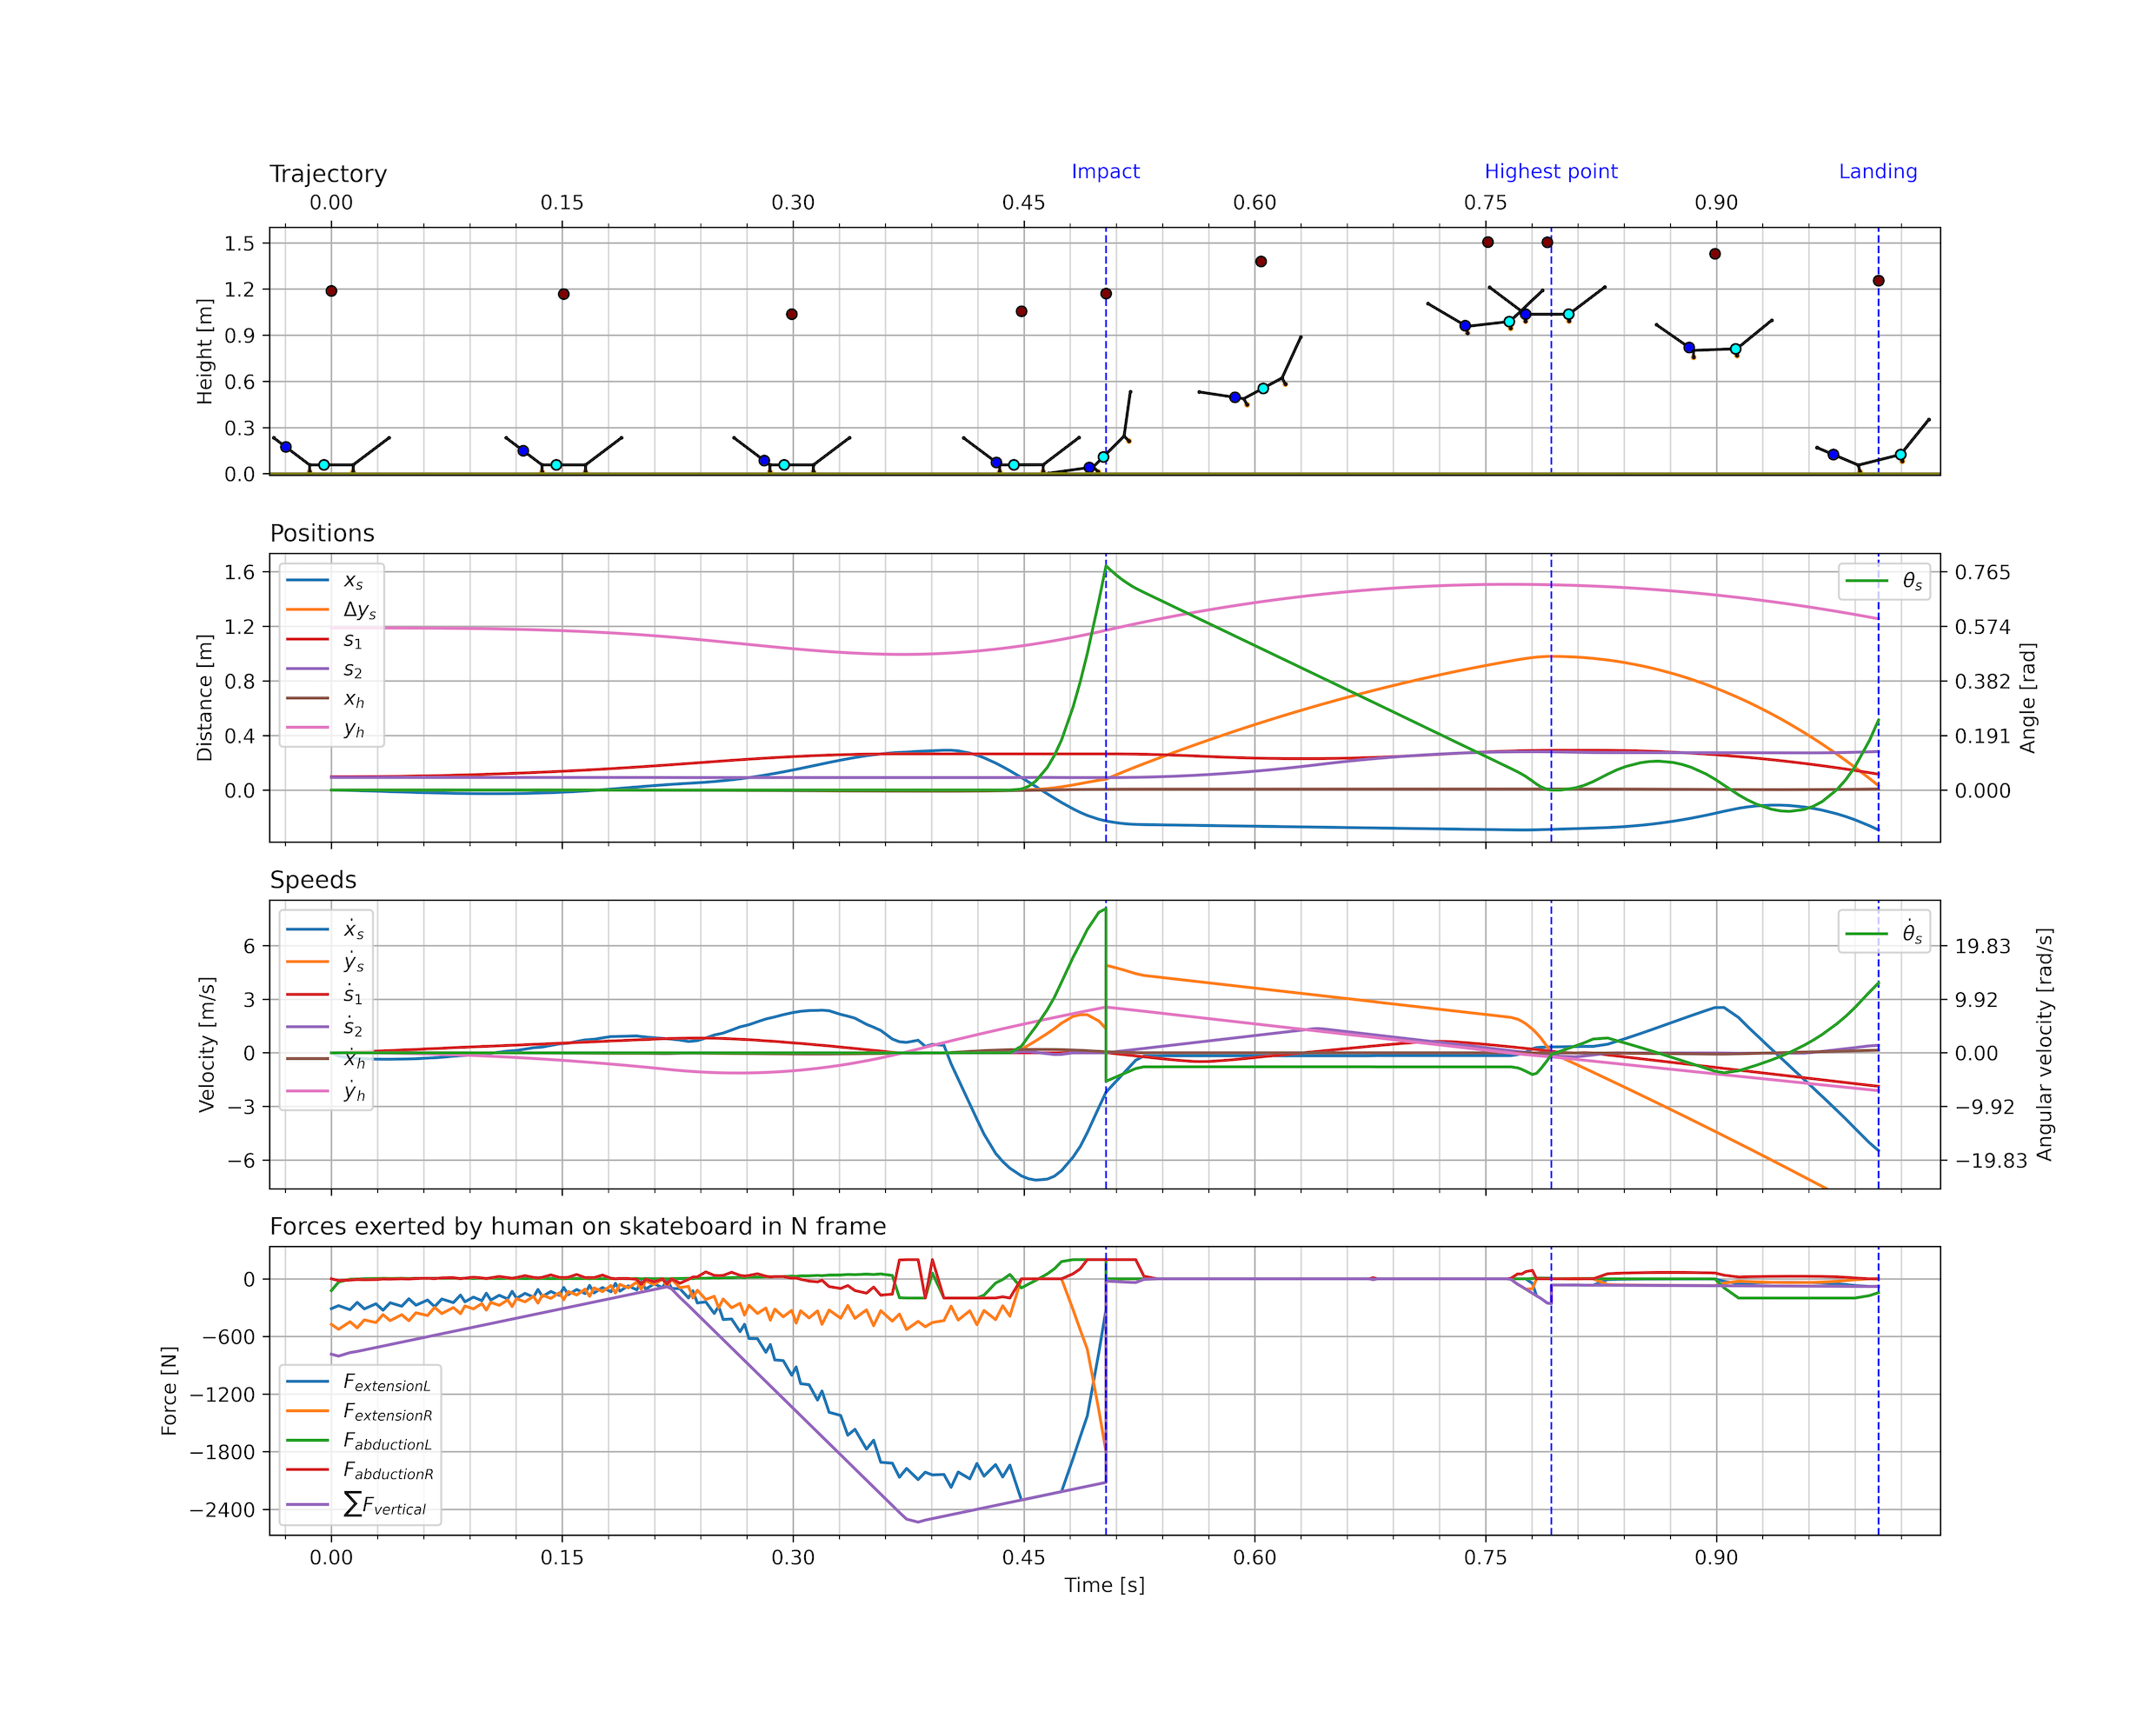
\includegraphics[trim={0cm 0cm 0cm 0cm},clip,width=0.8\textwidth]{figure/Results/data_alldpi600.png}}
    \caption{Tail inclination and all parameters optimization results}    
\end{figure*}


%Appendix will include inertia experiments and friction experiments

%% SHOW THAT NOSE ISN'T USED WHEN THE POSSIBILITY IS THERE

%% SHOW HOW VELOCITIES AFTER IMPACT ARE CALCULATED

%% SHOW 3 Friciton models
% During impact, friction can be present when there is a tangential velocity state relative to the impact surface. Poissons method and Newtons method have been shown unaccurate for such events and it is advised to use Stronge's method. This has been shown numerically in Stronge's comment on collision with friction\cite{stronge_comment_2010}. When the tail of the skateboard hits the ground, usually there is a tangential velocity state at the location of impact. This means that in real life a frictional impact occurs. Another implementation of the Poisson method during a frictional impact is solved with a set of constraints in the optimization\cite{patel_contact-implicit_2019}. The theory is that you create a variable $\phi(q_i)$, that represents the distance from the contact surface dependant on the generalized coordinates which should always be greater than 0. Furthermore there are three forces that should obey the friction cone presented in 

\end{document}
